%%%%%%%%%%%%%%%%%%%%%%%%%%%%%%%%%%%%%%%%%
% Masters/Doctoral Thesis 
% LaTeX Template
% Version 2.5 (27/8/17)
%
% This template was downloaded from:
% http://www.LaTeXTemplates.com
%
% Version 2.x major modifications by:
% Vel (vel@latextemplates.com)
%
% This template is based on a template by:
% Steve Gunn (http://users.ecs.soton.ac.uk/srg/softwaretools/document/templates/)
% Sunil Patel (http://www.sunilpatel.co.uk/thesis-template/)
%
% Template license:
% CC BY-NC-SA 3.0 (http://creativecommons.org/licenses/by-nc-sa/3.0/)
%
%%%%%%%%%%%%%%%%%%%%%%%%%%%%%%%%%%%%%%%%%

%----------------------------------------------------------------------------------------
%	PACKAGES AND OTHER DOCUMENT CONFIGURATIONS
%----------------------------------------------------------------------------------------

\documentclass[
11pt, % The default document font size, options: 10pt, 11pt, 12pt
%oneside, % Two side (alternating margins) for binding by default, uncomment to switch to one side
english, % ngerman for German
singlespacing, % Single line spacing, alternatives: onehalfspacing or doublespacing
%draft, % Uncomment to enable draft mode (no pictures, no links, overfull hboxes indicated)
%nolistspacing, % If the document is onehalfspacing or doublespacing, uncomment this to set spacing in lists to single
%liststotoc, % Uncomment to add the list of figures/tables/etc to the table of contents
%toctotoc, % Uncomment to add the main table of contents to the table of contents
%parskip, % Uncomment to add space between paragraphs
%nohyperref, % Uncomment to not load the hyperref package
headsepline, % Uncomment to get a line under the header
%chapterinoneline, % Uncomment to place the chapter title next to the number on one line
%consistentlayout, % Uncomment to change the layout of the declaration, abstract and acknowledgements pages to match the default layout
]{MastersDoctoralThesis} % The class file specifying the document structure

\usepackage[utf8]{inputenc} % Required for inputting international characters
\usepackage[T1]{fontenc} % Output font encoding for international characters
\usepackage{multicol}

\usepackage{mathpazo} % Use the Palatino font by default
\usepackage{appendix}
\usepackage{chngcntr}
\usepackage{etoolbox}
\usepackage{amsmath}
\usepackage{bm}
\usepackage{physics}
%\usepackage[demo]{graphicx}
\usepackage{caption}
\usepackage{subcaption}

\usepackage[backend=bibtex,natbib=true,sorting=none]{biblatex} % Use the bibtex backend with the authoryear citation style (which resembles APA)

\addbibresource{MT.bib} % The filename of the bibliography

\usepackage[autostyle=true]{csquotes} % Required to generate language-dependent quotes in the bibliography

%----------------------------------------------------------------------------------------
%	MARGIN SETTINGS
%----------------------------------------------------------------------------------------

\geometry{
	paper=a4paper, % Change to letterpaper for US letter
	inner=2.5cm, % Inner margin
	outer=3.8cm, % Outer margin
	bindingoffset=.5cm, % Binding offset
	top=1.5cm, % Top margin
	bottom=1.5cm, % Bottom margin
	%showframe, % Uncomment to show how the type block is set on the page
}

%----------------------------------------------------------------------------------------
%	THESIS INFORMATION
%----------------------------------------------------------------------------------------

\thesistitle{Ultrafast manipulation of Heisenberg exchange and Dzyaloshinskii–Moriya interactions in antiferromagnetic insulators} % Your thesis title, this is used in the title and abstract, print it elsewhere with \ttitle
\supervisor{Dr. James \textsc{Smith}} % Your supervisor's name, this is used in the title page, print it elsewhere with \supname
\examiner{} % Your examiner's name, this is not currently used anywhere in the template, print it elsewhere with \examname
\degree{Doctor of Philosophy} % Your degree name, this is used in the title page and abstract, print it elsewhere with \degreename
\author{Juan Manuel Losada} % Your name, this is used in the title page and abstract, print it elsewhere with \authorname
\addresses{} % Your address, this is not currently used anywhere in the template, print it elsewhere with \addressname

\subject{Biological Sciences} % Your subject area, this is not currently used anywhere in the template, print it elsewhere with \subjectname
\keywords{} % Keywords for your thesis, this is not currently used anywhere in the template, print it elsewhere with \keywordnames
\university{NTNU} % Your university's name and URL, this is used in the title page and abstract, print it elsewhere with \univname
\department{\href{http://department.university.com}{Department or School Name}} % Your department's name and URL, this is used in the title page and abstract, print it elsewhere with \deptname
\group{\href{http://researchgroup.university.com}{Research Group Name}} % Your research group's name and URL, this is used in the title page, print it elsewhere with \groupname
\faculty{\href{http://faculty.university.com}{Faculty Name}} % Your faculty's name and URL, this is used in the title page and abstract, print it elsewhere with \facname

\AtBeginDocument{
\hypersetup{pdftitle=\ttitle} % Set the PDF's title to your title
\hypersetup{pdfauthor=\authorname} % Set the PDF's author to your name
\hypersetup{pdfkeywords=\keywordnames} % Set the PDF's keywords to your keywords
}

% Start of subappendices environment
\AtBeginEnvironment{subappendices}{%
\chapter*{Appendices}
\addcontentsline{toc}{chapter}{Appendices}
\counterwithin{figure}{section}
\counterwithin{table}{section}
}

% End of subappendices environment
\AtEndEnvironment{subappendices}{%
\counterwithout{figure}{section}
\counterwithout{table}{section}
}

\newcommand{\bs}[1] {\boldsymbol{#1}}
\newcommand{\n}{\nonumber}

\begin{document}

\frontmatter % Use roman page numbering style (i, ii, iii, iv...) for the pre-content pages

\pagestyle{plain} % Default to the plain heading style until the thesis style is called for the body content

%----------------------------------------------------------------------------------------
%	TITLE PAGE
%----------------------------------------------------------------------------------------

\begin{titlepage}
\begin{center}

\vspace*{.06\textheight}
{\scshape\LARGE \univname\par}\vspace{1.5cm} % University name
\textsc{\Large Master Thesis}\\[0.5cm] % Thesis type

\HRule \\[0.4cm] % Horizontal line
{\huge \bfseries \ttitle\par}\vspace{0.4cm} % Thesis title
\HRule \\[1.5cm] % Horizontal line
 
\begin{minipage}[t]{0.4\textwidth}
\begin{flushleft} \large
\emph{Author:}\\
Juan Manuel Losada
\end{flushleft}
\end{minipage}
\begin{minipage}[t]{0.4\textwidth}
\begin{flushright}
\emph{Supervisor:} \\
Arne Brataas

\emph{Co-supervisor:}\\
Alireza Qaiumzadeh
\end{flushright}

\end{minipage}\\[3cm]
 
\end{center}
\end{titlepage}

\tableofcontents % Prints the main table of contents

\mainmatter % Begin numeric (1,2,3...) page numbering
\pagestyle{thesis} % Return the page headers back to the "thesis" style

\chapter{AFM spinotronics}

\section{History and background}

Antiferromagnetism was first studied by L. N\'eel who introduced a thermodinamic theory that made it possible to explain the antiferromagnetic order and it pretict the existance of a temperature above which this order vanishes. This temperature is known as N\'eel temperature. In the next section we will present a semiclassical model for antiferromagnetic materials.

During several decades after the discovery of antiferromagnetics, these materials were percived as useless from a practical point of view.On contrast, ferromagnets have been widely studied historically for its technical applications. However, in the frame of spinotronic devices, the development of information technology demands devices with high storage density, high energy efficiency and high write-read speeds. Therefore, controlling magnetically ordered systems on subpicosecond timescales is currently a widely studied area. Some progress has been done using ferromagnetic materials, for example, it has been shown that circularly polarized femtosecond laser pulses can be used to control the spin dynamics in magnets \cite{Kimel2005}. However, antiferromagnets aim to complement or even replace ferromagnets due to their rigidity to external magnetic field, and the abscence of stray field.

It has been shown that spin-transfer torques and giant magnetoresistance effects can occur in circuits containing only normal and antiferromagnetic materials \cite{MacDonald2011}. Additionally, spin axis reorientation by a lateral electrical current can be used to offer ultra-fast electrical writing and reading in AFM devices \cite{Zelezny2014}.


\chapter{Basic models for solid state}
\label{ChapBasicModels}

Many properties of solids can be understood using one-electron models, that is, non-interacting models. When the interaction between the ions and the valence electrons can be mostly neglected one can adapt the free electron approximation. This model is mostly limited to the study of metals and despite its simplicity it successfully explains phenomena related with electrical conductivity and heat capacity. In the opposite limit, we can consider systems in which the ion potential is so large that the electrons are bound in the cores with occasional jumps from site to site. This is known as tight binding model and it can be used to study a wide variety of solids. It is typically used for calculations of the electronic band structure.

Despite the success of the single particle models, there are several phenomena which cannot be explained neglecting electron correlations. For example, high temperature superconductivity cannot be understood with these models. The Hubbard model is the simplest model including electron correlations and despite its simplicity it is not fully understood yet. In this Chapter we will outline the main features of the tight binding model and the Hubbard model, which are basic tools for any condensed matter researcher.

\section{Tight binding}

When the electrons are strongly localized in the atom cores, the wavefunction describing such an electron is similar to the corresponding atomic orbital. Therefore it is natural to consider linear superposition of atomic orbitals as an anstatz for the crystal electron states.

Let the atomic Hamiltonian be $\hat{H}_a(\bs{r}) = -\frac{\hbar^2\hat{p}^2}{2m} + V_a(\bs{r}-\bs{r}_n)$, where $\hbar$ is the reduced Planck constant, $m$ is the electron mass, $\hat{p}$ is the momentum operator and $V_a(\bs{r})$ is the atomic potential. Let $\phi_i(\bs{r})$ be the i-\textit{th} eigenstate of the atomic Hamiltonian with energy $E_i$. The crystal Hamiltonian is:

\begin{equation}
\label{CrystalHam}
\hat{H} = -\frac{\hbar^2p^2}{2m} + \sum_n V_a(\bs{r}-\bs{r}_n)
\end{equation}
An electron localized around the atom at $\bs{r}_n$ will mainly feel the potential of that atom, and the potential of the rest of the atoms will be a perturbation to the free atom problem. That is, we can spit \ref{CrystalHam} into:
\begin{equation}
\label{SplitCrystalHam}
\hat{H} = \hat{H}_a + v(\bs{r}-\bs{r}_n)
\end{equation}
Where $v(\bs{r}-\bs{r}_n) = \sum_{m \neq n} V_a(\bs{r}-\bs{r}_m)$ is a small perturbation. We can expect the crystal electron to retain the properties of the free atom electron, and so, it is natural to describe the crystal electron as a superposition of atomic orbitals. Thus, we will try to find solutions of the form:

\begin{equation}
\psi_i(\bs{r}) = \sum_n b_i(\bs{r}_n) \phi_i(\bs{r}-\bs{r}_n)
\end{equation}
Now, the Bloch theorem states that an eigenfunction of the crystal Hamiltonian should only change by a phase from site to site, that is $\psi_i(\bs{r}+\bs{r}_m)=e^{i \bs{k} \cdot \bs{r}_m}\psi_i(\bs{r})$, where $\bs{k}$ is the crystal momentum of the Bloch wave. We can see that see implies $b_i(\bs{r}_m) = e^{i \bs{k} \cdot \bs{r}_m}b_i(0)$, by normalizing $\psi_i(\bs{r})$ we find $b_i(0) = \frac{1}{\sqrt{N}}$, where $N$ is the number of atoms in the crystal. We therefore obtain:

\begin{equation}
\psi_{i\bs{k}}(\bs{r}) = \frac{1}{\sqrt{N}}\sum_n  e^{i \bs{k} \cdot \bs{r}_n} \phi_i(\bs{r}-\bs{r}_n)
\end{equation}
The energy of this state is $E_i(\bs{k}) = \bra{\psi_{i\bs{k}}} \hat{H} \ket{\psi_{i\bs{k}}}$, using \ref{SplitCrystalHam} this can be written as:

\begin{equation}
E_i(\bs{k}) = \frac{1}{N} \sum_{n,m} e^{i\bs{k}\cdot(\bs{r}_n-\bs{r}_m)} \int \phi_i^*(\bs{r}-\bs{r}_m) (E_i+v(\bs{r}-\bs{r}_n)) \phi_i(\bs{r}-\bs{r}_n) d\bs{r}
\end{equation}
Assuming that $\phi_i$ is spherically symmetric, and neglecting the perturbation $v(\bs{r}-\bs{r}_n)$ further away than nearest neighbors, we can simplify this expression to:

\begin{equation}
\label{TBBand}
E_i(\bs{k}) = E_i - A - B\sum_{\bs{\delta}} e^{i\bs{k}\cdot \bs{\delta}}
\end{equation}
Where $\bs{\delta}$ are the NN vectors and:
\begin{align*}
A &= -\bra{\phi_i(\bs{r}-\bs{r}_n)}v(\bs{r}-\bs{r}_n) \ket{\phi_i(\bs{r}-\bs{r}_n)} \\
B &= -\bra{\phi_i(\bs{r}-\bs{r}_m)}v(\bs{r}-\bs{r}_n) \ket{\phi_i(\bs{r}-\bs{r}_n)}
\end{align*}
$A$ measures the amount of energy reduced when the atom forms a crystal, $B$ is a measure of the width of the band. 
In second quantization formalism we can write the tight binding single band Hamiltonian as:

\begin{equation}
\label{TBModel}
\hat{H} = -t\sum_{\langle i,j \rangle \sigma} \hat{c}^{\dagger}_{i\sigma}\hat{c}_{j\sigma}
\end{equation}
Where $\hat{c}^{\dagger}_{i\sigma}$ ($\hat{c}_{i\sigma}$) creates (annihilates) an electron in site $i$ and spin state $\sigma$. The quantity $t$ is the hopping amplitude, and plays the same role $B$ in the first quantization formalism. We can obtain back \ref{TBBand} by changing basis to momentum space $\hat{c}_{k\sigma} = \frac{1}{\sqrt{N}}\sum_j e^{-i\bs{k}\cdot\bs{r}_j}\hat{c}_{j\sigma}$. In Appendix \ref{APD} we use this formalism to compute the band structure of a two dimensional system in a honeycomb lattice (i.e. graphene).



\section{The Hubbard model}

As we discuss earlier, even tough the tight binding model is successful in describing the band structure of most solids, it fails in some cases. In strongly correlated electron systems, the effect of electron-electron Coulomb interactions is important, and this effect is neglected in \ref{TBModel}. The simplest way to take this effect into account is to consider the interaction of electrons in the same site only, that is, adding a term of the form $\text{U}\sum_i \hat{n}_{i\uparrow}\hat{n}_{i\downarrow}$, where $\text{U}$ is a constant accounting for the onsite electron-electron interaction:
\begin{equation}
\label{HH}
\hat{H} = -t\sum_{\langle i,j \rangle \sigma} \hat{c}^{\dagger}_{i\sigma}\hat{c}_{j\sigma} + \text{U}\sum_i \hat{n}_{i\uparrow}\hat{n}_{i\downarrow}
\end{equation}
This is known as the Hubbard model, which was first proposed by Hubbard \cite{Hubbard1963} to describe electron correlations in $d$ or $f$ bands in transition metals. The result was a simplified model to predict metal-insulator transitions. However, it exhibits much richer phenomena. It can be considered an impoved tight binding model, describing Mott insulators, which cannot be describied by band theory (i.e. they should be conductors according to band theory, but electron-electron interactions keep away from). Also, the attractive Hubbard model (where $\text{U} < 0$) can be considered an effective model relevant for understanding high temperature superconductivity \cite{Alexandrov1981}. Despite its simplicity the ground state has no analytic form in more than one dimensions, and different computational methods must be used to study it.

 Figure \ref{fig:Hubbard} shows a graphical representation of the parameters in \ref{HH}. The new term $\text{U}\sum_i \hat{n}_{i\uparrow}\hat{n}_{i\downarrow}$ will add an energy $+\text{U}$ when a site is double occupied ($\hat{n}_{i\uparrow} = \hat{n}_{i\downarrow} = 1$) and will not contribute in the more normal case, that $\hat{n}_{i\uparrow} + \hat{n}_{i\downarrow} = 1$. The half-filled case is most commonly studied, this is the situation where the system has one electron per site (or it has half the maximum allowed number). This situation is simpler in many ways and it exhibits a lot of interesting phenomena (Mott insulating behavior, antiferromagnetic order, etc.). However, other cases have also been widely studied.

\begin{figure}
\centering
  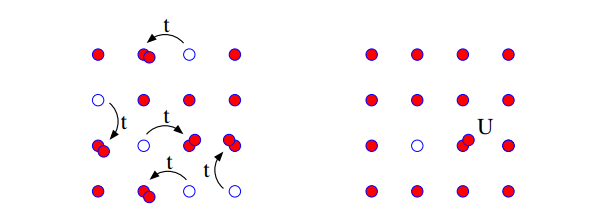
\includegraphics[width=\linewidth]{../Figures/hubbard.png}
  \caption{Image from Scalettar's notes representing the kinetic term $t$ and the on-site interaction $\text{U}$ in the Hubbard model.} 
\label{fig:Hubbard}
\end{figure}
Notice that if we set $\text{U}=0$ in \ref{HH} we recover the tight binding Hamiltonian, therefore we can say that the Hubbard model is an expansion of the tight binding model. The opposite limit $t=0$ is more interesting. In the half-filling case, for $\text{U}>0$ the ground state will be any state with exactly one electron per site. Since each electron can be in two spin states there is a $2^N$ degeneracy. The subspace spanned by these states is referred to as low energy subspace, and in this case is has energy $E_0 = 0$. If we switch $0 \neq t \ll \text{U}$ this hopping term will allow an even further decrease in energy by allowing virtual processes $i \rightarrow j \rightarrow i$ that localized the electrons withing their neighbor sites. For $t \ll \text{U}$ the dynamics of the system can be described withing the low energy subspace only, by doing so we can obtain an effective spin Hamiltonian $\hat{H}_{\text{eff}} = \sum{\langle i,j \rangle} J \bs{S}_i\cdot\bs{S}_j$ where $J>0$ describing an antiferromagnetic system. A rigorous derivation of this will be offered in the next Chapter, however we can intuitively understand this result in the following way: the virtual processes $i \rightarrow j \rightarrow i$ will be allowed when the electrons at sites $i$ and $j$ have opposite spin (otherwise it would contradict the Pauli principle), therefore states where neighbor sites have opposite spins will have a lower energy due to the delocalization mechanism. Additionally, the constant $J$ will be proportional to the amplitude of the process $i \rightarrow j \rightarrow i$. We can already see that this amplitude is $2\frac{t^2}{\text{U}}$, $t^2$ due to two hopping processes, $\frac{1}{\text{U}}$ due to the energy of the intermediate state and the factor $2$ due to the two spin possibilities.

In the next Chapter and in the rest of this thesis we will consider the effects of spin orbit interaction (SOI) in strongly correlated systems. For this reason we will have an additionally spin dependent hopping term in \ref{HH} arising from the SOI. This additional term will lead to a DMI when deriving the effective spin Hamiltonian in the $t \ll \text{U}$ limit.







\chapter{Effective Spin Hamiltonian}

In this chapter we will start with a Hamiltonian

\begin{equation}
\label{Ham1}
\hat{H} = \sum_{i=1}^{N_e} \hat{H}^{(1)}(\textbf{r}_i) + \frac{1}{2} \sum_{\substack{i,j = 1 \\ i \neq j}} ^ {N_e} v(\textbf{r}_i - \textbf{r}_j)
\end{equation}

where $v$ is the electron-electron interaction and where $\hat{H}^{(1)}$ is the single particle Hamiltonian:

\begin{equation}
\hat{H}^{(1)}(\textbf{r}) = -\frac{\hbar^2}{2m}\nabla^2_{\textbf{r}} + \text{U}(\textbf{r}) + \lambda\bs{\sigma}\cdot\bs{\nabla}V(\textbf{r}) \times \textbf{p}
\end{equation}

Where $\lambda = \frac{\hbar^2}{4m^2c^2}$ is the spin orbit coupling constant and $\text{U}(\bs{r})$ is a periodic potential. The second quantized form of this Hamiltonian can be approximated by a version of the Hubbard model. The original Hubbard model, was developed to describe the single-band magnetism \cite{Hubbard1963}, it also describes the transition between conducting and insulating systems, predicting the existence of Mott insulators, materials which should be conducting according to band theory, but they are insulating due to electron-electron interactions.

We will consider a half filled system in the strong coupling limit. Ignoring electron hopping and spin orbit interaction, the ground state of this system is massively degenerated. We will find an effective Hamiltonian considering that the hopping term and the spin interaction term act on this subspace. This effective Hamiltonian will be the sum of three spin interactions: an exchange interaction $J\bs{S}_i\cdot\bs{S}_j$ with $J>0$, a Dzyaloshinkii-Moriya interaction $\bs{D}\bs{S}_i\times\bs{S}_j$ and an anisotropic interaction $\bs{S}_i \bs{\Gamma} \bs{S}_j$ known as pseudodipolar interaction \cite{Moriya1960}.

\begin{section}{Single particle in a periodic potential}

First we will define a suitable basis for the single particle wavefunctions. To do so, we will consider the single particle Hamiltonian without the spin orbit interaction term:

\begin{equation}
\label{LaticeHam}
\hat{H}^{(1)}_{\text{NSOI}}(\textbf{r}) = -\frac{\hbar^2}{2m}\nabla^2_{\textbf{r}} + \text{U}(\textbf{r})
\end{equation}

Where $\text{U}(\bs{r})$ has the symmetry of the lattice, i.e. $\text{U}(\bs{r} + \bs{R}) = \text{U}(\bs{r})$ for all Bravais lattice vectors $\bs{R}$(\ref{AP1A}). Let $\hat{H}^{(1)}_{\text{NSOI}}$ act on a Hilbert space $\mathcal{H}$ and let $\ket{\phi} \in \mathcal{H}$, then, the group of translation symmetries defined by $\bra{\bs{r}} T_{\bs{R}} \ket{\phi} = \bra{\bs{r} + \bs{R}} \ket{\phi}$ is an abelian group, therefore its irreducible representations are one-dimensional, that is, within an energy level $n$ the wavefunctions of that level transform according to the representation they belong. If $\Gamma^{\bs{k}}$ is a one dimensional representation and $\ket{\phi_n, \bs{k}}$ is a wavefunction in the energy level $n$ belonging to that representation then $T_{\bs{R}}\ket{\phi_{n, \bs{k}}} = \Gamma^{\bs{k}}(\bs{R}) \ket{\phi_{n, \bs{k}}}$. Now, imposing periodic boundary conditions, $\Gamma^{\bs{k}}(\bs{a}_\mu)^{L_\mu} = 1$, where $\bs{a}_\mu$ are the primitive translations and $L_\mu$ is the number of lattice sites in the $\mu$ direction as defined in \ref{AP1A}. This can be accomplished if we label the representation with a vector of the first Brillouin zone and have $\Gamma^{\bs{k}}(R) = e^{i \bs{k} \cdot \bs{R}}$. Therefore, for a wavefunction in a periodic lattice we have:

\begin{equation}
\label{Bloch1}
\bra{\bs{r}+\bs{R}} \ket{\phi_{n, \textbf{k}}} = e^{i\bs{k}\cdot\bs{R}}\bra{\bs{r}} \ket{\phi_{n, \textbf{k}}}
\end{equation}

Which is the well-known Bloch function form. Here, $n$ is called the band index, and $\textbf{k}$ is the quasimomentum. The energy of this wavefunction is $\epsilon_{n \textbf{k}}$.  Notice that both $\phi_{n,\textbf{k}}$ and $\epsilon_{n \textbf{k}}$ are periodic functions of $\textbf{k}$ in the reciprocal lattice.

The Bloch function is extended over the whole crystal volume $V$. We would like to work with a localized basis. An alternative orthonormal basis are the Wannier functions $\ket{\psi_{in}}$, defined in terms of the Bloch functions as:

\begin{align}
\bra{\bs{r}}\ket{\phi_{n\bs{k}}} &= \frac{1}{\sqrt{M}}\sum_{\bs{R}} e^{i\bs{k}\cdot\bs{R}} \bra{\bs{r}}\ket{\psi_{\bs{R}n}}  \label{Wannier1} \\
\bra{\bs{r}}\ket{\psi_{in}} &= \frac{1}{\sqrt{M}} \sum_{\bs{k}\in BZ} e^{-i\bs{k}\cdot\bs{R}_i} \bra{\bs{r}}\ket{\phi_{n\bs{k}}}\label{Wannier2}
\end{align}

Where $M$ is the number of lattice sites as defined in \ref{AP1A}. Using \ref{Bloch1} we see that $\psi_{in}(\textbf{r}) = \psi_{0n}(\textbf{r}-\textbf{r}_i) \equiv \psi_{n}(\textbf{r}-\textbf{r}_i)$, so we only need to define one Wannier function for each band and the others are obtained by translations. From now on we will restrict ourselves to a fixed band, so we will drop the band index. Additionally, we will include the spin state, therefore the basis states will have two quantum numbers one for the site and one for the spin state. We will adopt the notation $\ket{i\sigma}$ for the basis state of site $i$ with spin state $\sigma = \uparrow, \downarrow$, or just $\ket{i}$ when the spin state is irrelevant. Fock space states with small number of particles will be denoted as $\ket{i\sigma, j\sigma'}$, for a state with a particle at site $i$ with spin $\sigma$ and a particle at $j$ with spin $\sigma'$, or $\ket{ij}$ when spin is irrelevant.

\end{section}

\begin{section}{Derivation of the single-band Hubbard model}

In this section we will derive the second quantized form of \ref{Ham1} using the Wannier function basis. Let $\hat{c}_{j \sigma}^\dagger$ and $\hat{c}_{j \sigma}$ create and annihilate a particle in the state $\ket{j\sigma}$. In this basis, the second quantized form of \ref{Ham1} is:

\begin{equation}
\hat{H} = \sum_{i,j,\sigma, \sigma'} \bra{i\sigma} \hat{H}^{(1)} \ket{j\sigma'} \hat{c}_{i \sigma}^\dagger \hat{c}_{j \sigma'} + \frac{1}{2} \sum_{i,j,k,l, \sigma, \sigma'} \bra{ij} \hat{v} \ket{kl} \hat{c}_{i \sigma}^\dagger \hat{c}_{j \sigma'}^\dagger \hat{c}_{l \sigma'} \hat{c}_{k \sigma}
\end{equation}

Where we assumed $\hat{v}$ to be spin independent. This can be rewritten as:

\begin{equation}
\hat{H} = -\sum_{i,j,\sigma, \sigma'} (\delta_{\sigma, \sigma'} t_{ij} + \bs{\Delta}_{ij} \cdot\bs{\sigma}_{\sigma, \sigma'}) \hat{c}_{i \sigma}^\dagger \hat{c}_{j \sigma'} + \frac{1}{2} \sum_{i,j,k,l, \sigma, \sigma'} \bra{ij} \hat{v} \ket{kl} \hat{c}_{i \sigma}^\dagger \hat{c}_{j \sigma'}^\dagger \hat{c}_{l \sigma'} \hat{c}_{k \sigma}
\end{equation}

Where $t_{ij} = -\bra{i} -\frac{\hbar^2}{2m}\nabla^2_{\textbf{r}} + \text{U}(\textbf{r}) \ket{j}$ and $\boldsymbol{\Delta}_{ij} = -\bra{i} \lambda \boldsymbol{\nabla}V(\textbf{r}) \times \textbf{p} \ket{j}$. Notice that $\bs{\Delta}_{ij} = - \bs{\Delta}_{ji}$, for example, in the $x$ component:

\begin{align*}
\Delta_{ij,x} &= -\bra{i} \lambda (\partial_y V(\bs{r}) p_z - \partial_z V(\bs{r}) p_y) \ket{j} = i \hbar \lambda \int d \bs{r} \phi_i(\bs{r})^* (\partial_y V(\bs{r}) \partial_z - \partial_z V(\bs{r}) \partial_y) \phi_j(\bs{r}) = \\
&= -i\hbar\lambda \int d\bs{r} \left[ \partial_z(\phi_i(\bs{r})^*\partial_y V(\bs{r}) - \partial_y(\phi_i(\bs{r})^*\partial_z V(\bs{r}) \right] \phi_j(\bs{r}) = \\
&= -i\hbar\lambda \int d\bs{r} \left[ \partial_z \phi_i(\bs{r})^* \partial_y V(\bs{r}) - \partial_y \phi_i(\bs{r})^*\partial_z V(\bs{r}) \right] \phi_j(\bs{r}) = \\
&= \int d\bs{r} \phi_j(\bs{r}) \lambda (\bs{\nabla}V(\bs{r}) \times \bs{p})_x \phi_i(\bs{r})^* = - \Delta_{ji,x}
\end{align*}

Therefore $\bs{\Delta}_{ii} = 0$. Notice also that $\bs{\Delta}_{ij}$ is purely imaginary.
We can impose that $t_{ii} = t(0) = 0$. For a system of strongly correlated electrons we can assume that:

\begin{itemize}
\item A property of the Wannier functions $\Phi_j$ is that they have exponentially decreasing overlaps, therefore $t_{ij}$ and $\boldsymbol{\Delta}_{ij}$ will decay rapidly with the distance $|\textbf{r}_i-\textbf{r}_j|$. In an isotropic system we can approximate:

\begin{equation}
t_{ij} = \begin{cases}
             t,  & \text{for } (i,j) \text{ nearest neighbous} \\
             0,  & \text{otherwise}
       \end{cases} \quad
\end{equation}

and

\begin{equation}
\bs{\Delta}_{ij} = \begin{cases}
             \bs{\Delta}_{ij},  & \text{for } (i,j) \text{ nearest neighbours} \\
             0,  & \text{otherwise}
       \end{cases} \quad
\end{equation}

Hubbard models with hopping terms further than nearest neighbors are also interesting and will be considered in next chapter.  

\item Taking into account the locality of the Wannier functions and the Coulomb interaction, the dominant contribution of $\bra{ij} \hat{v} \ket{kl}$ will come from $i=j=k=l$. Terms with $i=k$ and $j=l$ also contribute when $i, j$ are nearest neighbours. Therefore we approximate:

\begin{equation}
\bra{ij} \hat{v} \ket{kl} =
	\begin{cases}
		\text{U}, & \text{if } i=j=k=l \\
		\text{V}, & \text{if } i=k \text{ and } j=l \text{ where } (i,j) \text{ nearest neighbours} \\
		0, & \text{otherwise}
	\end{cases}						
\end{equation}

Where we defined:

\begin{align}
\text{U} &= \frac{1}{2} \int d\bs{r} d\bs{r}' \phi(\bs{r})^* \phi(\bs{r}')^* \hat{v}(\bs{r}-\bs{r}') \phi(\bs{r}') \phi(\bs{r}) \\
\text{V} &= \int d\bs{r} d\bs{r}' \phi(\bs{r})^* \phi(\bs{r}'-\bs{R}_1)^* \hat{v}(\bs{r}-\bs{r}') \phi(\bs{r}'-\bs{R}_1) \phi(\bs{r})
\end{align}

Where $\phi(\bs{r})$ is the Wannier function centered at the origin and $\bs{R}_1$ is a nearest neighbour lattice vector. Notice that we made explicit use of the translational invariance of the system. Also, for $i=j=k=l$ the Pauli principle requires $\sigma' = -\sigma$.

\end{itemize}

Taking these approximations and writing $\hat{c}_{i \sigma}^\dagger \hat{c}_{j \sigma'}^\dagger \hat{c}_{j \sigma'} \hat{c}_{i \sigma} = \hat{n}_{i \sigma} \hat{n}_{j \sigma'}$, we obtain:

\begin{equation}
\label{HubbardWithNonLocalInt}
\hat{H} = -\sum_{\langle i,j \rangle, \sigma, \sigma'}(\delta_{\sigma, \sigma'} t_{ij} + \bs{\Delta}_{ij} \cdot \bs{\sigma}_{\sigma, \sigma'})\hat{c}_{i \sigma}^\dagger \hat{c}_{j \sigma'} + \text{U} \sum_{i=1}^M \hat{n}_{i\uparrow}\hat{n}_{i\downarrow} + \text{V} \sum_{i,j,\sigma,\sigma'}  \hat{n}_{i \sigma} \hat{n}_{j \sigma'}
\end{equation}

Now, in a half filling system this Hamiltonian can be well approximated by an effective Hamiltonian without non local Coulomb interactions:

\begin{equation}
\label{Intermediate}
\hat{H} = -\sum_{\langle i,j \rangle, \sigma, \sigma'}(\delta_{\sigma, \sigma'} t_{ij} + \bs{\Delta}_{ij} \cdot\bs{\sigma}_{\sigma, \sigma'})\hat{c}_{i \sigma}^\dagger \hat{c}_{j \sigma'} + \text{U}^* \sum_{i=1}^M \hat{n}_{i\uparrow}\hat{n}_{i\downarrow}
\end{equation}

Where $\text{U}^* = \text{U} - \text{V}$. The physical reason for this is that the energy difference when the Coulomb interaction pushes an electron from a double occupied site to an empty site is $\text{U}-\text{V}$ in \ref{HubbardWithNonLocalInt}, because the number of double occupied sites is reduced by one but the number of adjacent occupied sites is increased by one. This is illustred in Figure \ref{Fig2.1}. A more rigouros derivation of this effective model can be found in \cite{Schuler2013}. Altough $\text{V} < \text{U}$, they can be comparable in magnitude, and $\text{U}^*$ can be reduced by a factor of $0.5$ or more.

\begin{figure}
\centering
  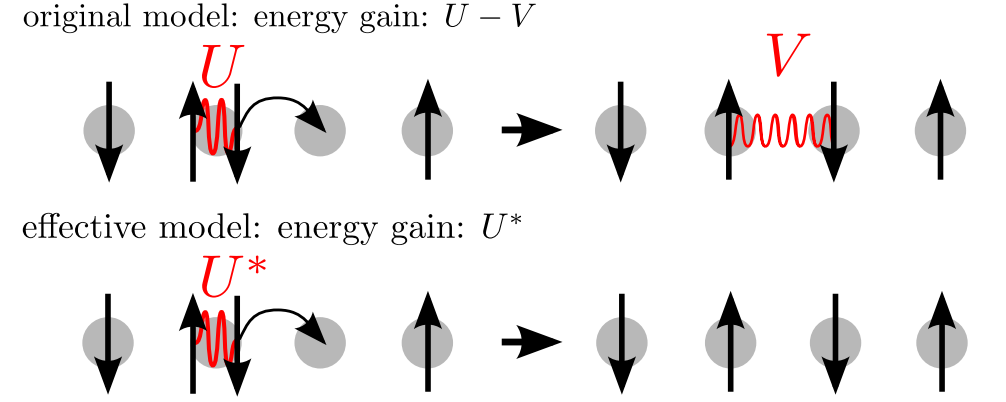
\includegraphics[width=0.5\linewidth]{../Figures/non_local_coulomb.png}
  \caption{Image from \cite{Schuler2013}. In a half-filled system decreasing the number of double occupancies increases the number of adjacent occupied sites, and so the energy difference is reduced to $\text{U}-\text{V}$.} 
\label{Fig2.1}
\end{figure}

Now, abusing the notation and writing $\text{U} = \text{U}^*$ we arrive at the model that we will use in the next sections:

\begin{equation}
\label{Hubbard}
\hat{H} = -\sum_{\langle i,j \rangle, \sigma, \sigma'}(\delta_{\sigma, \sigma'} t_{ij} + \bs{\Delta}_{ij} \cdot \bs{\sigma}_{\sigma, \sigma'})\hat{c}_{i \sigma}^\dagger \hat{c}_{j \sigma'} + \text{U} \sum_{i=1}^M \hat{n}_{i\uparrow}\hat{n}_{i\downarrow}
\end{equation}

\begin{subsection}{Hubbard model}

In the absence of spin-orbit interaction the model \ref{Hubbard} becomes the well-known Hubbard model: $\hat{H} = -\sum_{\langle i,j \rangle, \sigma} t_{ij} \hat{c}_{i \sigma}^\dagger \hat{c}_{j \sigma} + \text{U} \sum_{i=1}^M \hat{n}_{i\uparrow}\hat{n}_{i\downarrow}$. This model has been extensively studied since its proposal in 1963 by Hubbard \cite{Hubbard1963}. Despite its simplicity the ground state has no analytic form in more than one dimensions, and different computational methods must be used to study it. Originally the Hubbard model was proposed to describe electron correlations in $d$ or $f$ bands in transition metals. The result was a simplified model to predict metal-insulator transitions. However, it exhibits much richer phenomena. It can be considered an impoved tight binding model, describing Mott insulators, which cannot be describied by band theory (i.e. they should be conductors according to band theory, but electron-electron interactions keep away from). Also, the attractive Hubbard model (where $\text{U} < 0$) can be considered an effective model relevant for understanding high temperature superconductivity \cite{Alexandrov1981}.

\end{subsection}

\end{section}

\begin{section}{Effective Hamiltonian for half-filling system}

At half filling and in the $t << \text{U}$ limit, which correspond to the strong coupling limit, we can apply perturbation theory to obtain the Heisenberg model from the Hubbard Hamiltonian \ref{Hubbard}. First notice that in the case $t = 0$ the ground state corresponds to having all sites single-occupied. There are two possible spin orientations for each sites, so there is a $2^M$ degeneracy. The ground state energy is $0$. The first exited states are obtained by moving one electron from one site to another, thus leaving one empty site and one double-occupied site. The energy of one of these states is $\text{U}$. Now, if we turn the kinetic term on as a perturbation, having two neighbors electrons with antiparallel spin will allow them to hop and reduce the kinetic energy, whereas while being parallel this hopping is not allowed and there is no energy reduction. Therefore, we can see that when turning the kinetic term on antiparallel alignment will be favored. 

Let us write $\hat{H} = \hat{H}_0 + \hat{H}_t$, where $\hat{H}_0$ is the Hamiltonian for $t=0$ i.e. $\hat{H}_0 = \text{U} \sum_{i=1}^M \hat{n}_{i\uparrow}\hat{n}_{i\downarrow}$ and $\hat{H_t} = -\sum_{\langle i,j \rangle, \sigma, \sigma'}(\delta_{\sigma, \sigma'} t + \bs{\Delta}_{ij}\cdot \bs{\sigma}_{\sigma, \sigma'})\hat{c}_{i \sigma}^\dagger \hat{c}_{j \sigma'}$. Let $\ket{\phi}$ and $\ket{\phi'}$ be states from the ground state of $\hat{H}_0$, then we know $\bra{\phi'} \hat{H_0} \ket{\phi} = 0$ and in first order in $t$ $\bra{\phi'} \hat{H} \ket{\phi} = \bra{\phi'} \hat{H_t} \ket{\phi} = 0$ since $\hat{c}_{i \sigma}^\dagger \hat{c}_{j \sigma}$ moves an electron from site $j$ to $i$ thus leaving $i$ doubly occupied, therefore $\hat{H_t} \ket{\phi}$ has no superposition with $\phi'$. In second order we have:

\begin{equation}
\bra{\phi'} \hat{H} \ket{\phi} = \sum_s \frac{\bra{\phi'} \hat{H_t} \ket{s}\bra{s} \hat{H_t} \ket{\phi}}{E_0-E_s}
\end{equation}

The sum being over all excited states. Since $\hat{H_t}\ket{\phi}$ is a superposition of states with exactly one double occupied site and one empty site, we see that only excited states with one double occupied site will contribute. These states have energy $E_s = \text{U}$ therefore we have $\bra{\phi'} \hat{H} \ket{\phi} = -\frac{1}{\text{U}}\sum_s \bra{\phi'} \hat{H_t} \ket{s}\bra{s} \hat{H_t} \ket{\phi} = \bra{\phi'} -\frac{\hat{H_t^2}}{\text{U}} \ket{\phi}$. This means that within the subspace generated by the ground states of $\hat{H_0}$, $\hat{H}$ acts as an effective Hamiltonian $\hat{H}_{\text{eff}} = -\frac{\hat{H_t^2}}{\text{U}}$. Now,

\begin{align}
\label{PertNoEMF}
&\bra{\phi'} -\frac{\hat{H_t^2}}{\text{U}} \ket{\phi} = \nonumber \\
&= -\frac{1}{\text{U}} \bra{\phi'}\sum_{\langle i,j \rangle, \sigma_1, \sigma_2} \sum_{\langle i',j' \rangle, 					\sigma_3, \sigma_4} \left( \delta_{\sigma_1, \sigma_2} t + \bs{\Delta}_{ij} \cdot\bs{\sigma}_{\sigma_1, \sigma_2} \right) \left( \delta_{\sigma_3, \sigma_4} t + \bs{\Delta}_{i'j'} \bs{\sigma}_{\sigma_3, \sigma_4} \right)\hat{c}_{i\sigma_1}^\dagger \hat{c}_{j \sigma_2} \hat{c}_{i' \sigma_3}^\dagger \hat{c}_{j'\sigma_4} \ket{\phi} = \nonumber \\
&= -\frac{1}{\text{U}} \bra{\phi'}\sum_{\langle i,j \rangle, \sigma_1, \sigma_2, \sigma_3, \sigma_4} \left( \delta_{\sigma_1, \sigma_2} t + \bs{\Delta}_{ij} \cdot\bs{\sigma}_{\sigma_1, \sigma_2} \right) \left( \delta_{\sigma_3, \sigma_4} t - \bs{\Delta}_{ij} \cdot\bs{\sigma}_{\sigma_3, \sigma_4} \right)\hat{c}_{i\sigma_1}^\dagger \hat{c}_{j \sigma_2} \hat{c}_{j \sigma_3}^\dagger \hat{c}_{i\sigma_4} \ket{\phi} = \nonumber \\
&-\frac{1}{\text{U}} \bra{\phi'} \sum_{\langle i,j \rangle, \sigma_1, \sigma_2, \sigma_3, \sigma_4} (t^2 						\delta_{\sigma_1 \sigma_2}\delta_{\sigma_3 \sigma_4} + t\bs{\Delta}_{ij}(\delta_{\sigma_3 \sigma_4}			\bs{\sigma}_{\sigma_1 \sigma_2} - \delta_{\sigma_1 \sigma_2} \bs{\sigma}_{\sigma_3 \sigma_4}) - (\bs{\Delta}_{ij}\bs{\sigma}_{\sigma_1 \sigma_2})(\bs{\Delta}_{ij} \cdot\bs{\sigma}_{\sigma_3 \sigma_4}) ) \hat{c}_{i\sigma_1}^\dagger \hat{c}_{i\sigma_4} \hat{c}_{j 		\sigma_2} \hat{c}_{j \sigma_3}^\dagger \ket{\phi} = \nonumber \\
& \bra{\phi'} \hat{H}_J + \hat{H}_D + \hat{H}_P \ket{\phi}
\end{align}

In the second line we imposed $i=j'$ and $j=i'$ since that's the only way $\hat{H_t^2}\ket{\phi}$ has no double occupied sites and so the matrix element does not vanish. We also used $\bs{\Delta}_{ij} = - \bs{\Delta}_{ji}$. We defined:

\begin{align}
\hat{H}_J &= -\frac{t^2}{\text{U}} \sum_{\langle i,j \rangle, \sigma, \sigma'} \hat{c}_{i\sigma}^\dagger \hat{c}_{i\sigma'} \hat{c}_{j\sigma} \hat{c}_{j \sigma'}^\dagger \\
\hat{H}_D &= -\frac{t}{\text{U}}\sum_{\langle i,j \rangle, \sigma_1, \sigma_2, \sigma_3, \sigma_4} \bs{\Delta}_{ij}(\delta_{\sigma_3 \sigma_4}	\bs{\sigma}_{\sigma_1 \sigma_2} - \delta_{\sigma_1 \sigma_2} \bs{\sigma}_{\sigma_3 	\sigma_4}) \hat{c}_{i\sigma_1}^\dagger \hat{c}_{i\sigma_4} \hat{c}_{j \sigma_2} \hat{c}_{j \sigma_3}^\dagger \\
\hat{H}_P &= \frac{1}{\text{U}}\sum_{\langle i,j \rangle, \sigma_1, \sigma_2, \sigma_3, \sigma_4} (\bs{\Delta}_{ij}\bs{\sigma}_{\sigma_1 \sigma_2})(\bs{\Delta}_{ij} \cdot\bs{\sigma}_{\sigma_3 \sigma_4}) \hat{c}_{i\sigma_1}^\dagger \hat{c}_{i\sigma_4} \hat{c}_{j \sigma_2} \hat{c}_{j \sigma_3}^\dagger
\end{align}

Let us now introduce the on-site spin operators:

\begin{equation}
\label{SpinOperators}
\boldsymbol{S}_i = \frac{1}{2} \sum_{\sigma, \sigma'} \hat{c}_{i \sigma}^\dagger \boldsymbol{\sigma}_{\sigma, \sigma'} \hat{c}_{i \sigma'}
\end{equation}

Which satisfy:

\begin{align}
\hat{c}_{i \sigma}^\dagger \hat{c}_{i \sigma'} &= \delta_{\sigma \sigma'} \frac{1}{2} (n_{i \uparrow} + n_{i \downarrow}) + \bs{S}_i\cdot\bs{\sigma}_{\sigma', \sigma} \label{SpinOperatorInv1}\\ 
\hat{c}_{i \sigma} \hat{c}_{i \sigma'}^\dagger &= \delta_{\sigma \sigma'} \frac{1}{2} (2 - n_{i \uparrow} - n_{i \downarrow}) - \cdot\bs{S}_i\bs{\sigma}_{\sigma, \sigma'} \label{SpinOperatorInv2}
\end{align}

In the half-filling case we have $n_{i \uparrow} + n_{i \downarrow} = 1$ and we can show two important relations. First:

\begin{align*}
&\sum_{\sigma \sigma'} \left(\frac{1}{2}\delta_{\sigma \sigma'} + \bs{S}_i\cdot\bs{\sigma}_{\sigma' \sigma}\right)\left(\frac{1}{2}\delta_{\sigma \sigma'}-\bs{S}_j\cdot\bs{\sigma}_{\sigma \sigma'}\right) = \sum_{\sigma \sigma'} \left\{ \frac{1}{4}\delta_{\sigma \sigma'} - \sum_{ab} S_i^aS_j^b 	\bs{\sigma}_{\sigma'\sigma}^a \cdot \bs{\sigma}_{\sigma \sigma'}^b \right\}= \\
&= \frac{1}{2} - \sum_{ab} S_i^aS_j^b	2\delta_{ab} = \frac{1}{2} - 2\bs{S}_i\cdot\bs{S}_j
\end{align*}

Where we have neglected the term $\sum_{\sigma \sigma'} \frac{1}{2}\delta_{\sigma,\sigma'}(\bs{S}_i\cdot\bs{\sigma}_{\sigma',\sigma} - \bs{S}_j\cdot\bs{\sigma}_{\sigma,\sigma'})$ because eventually we will sum over all $\langle i, j \rangle$ and it will cancel out. We also used the well known property $tr(\bs{\sigma}^a\bs{\sigma}^b)=2\delta_{a,b}$. And second:

\begin{align*}
&\sum_{\sigma_1, \sigma_2, \sigma_3, \sigma_4}\bs{\Delta}_{ij}\cdot(\delta_{\sigma_3 \sigma_4}\bs{\sigma}_{\sigma_1 \sigma_2} - \delta_{\sigma_1 \sigma_2} \bs{\sigma}_{\sigma_3\sigma_4})\left(\frac{1}{2}\delta_{\sigma_1 \sigma_4} + \bs{S}_i\cdot\bs{\sigma}_{\sigma_4 \sigma_1}\right)\left(\frac{1}{2}\delta_{\sigma_2 \sigma_3}-\bs{S}_j\cdot\bs{\sigma}_{\sigma_2 \sigma_3}\right) = \\
 &= \left\{ \right.
	\overbrace{0}^{\uparrow \uparrow \uparrow \uparrow} +
	\overbrace{(-\Delta_{ij}^+)S_i^-(\frac{1}{2}-S_j^z)}^{\uparrow \uparrow \uparrow \downarrow} +
	\overbrace{(-\Delta_{ij}^-)(\frac{1}{2}+ S_i^z)(-S_j^+)}^{\uparrow \uparrow \downarrow \uparrow} +
	\overbrace{2\Delta_{ij}^z S_i^-(-S_j^+)}^{\uparrow \uparrow \downarrow \downarrow} + \\
	&\overbrace{\Delta_{ij}^+ (\frac{1}{2}+S_i^z)(-S_j^-)}^{\uparrow \downarrow \uparrow \uparrow} +
	\overbrace{0}^{\uparrow \downarrow \uparrow \downarrow} +
	\overbrace{0}^{\uparrow \downarrow \downarrow \uparrow} +
	\overbrace{\Delta_{ij}^+ S_i^-(\frac{1}{2}+S_j^z)}^{\uparrow \downarrow \downarrow \downarrow} + \\
	&\overbrace{\Delta_{ij}^- S_i^+(\frac{1}{2}-S_j^z)}^{\downarrow \uparrow \uparrow \uparrow} +
	\overbrace{0}^{\downarrow \uparrow \uparrow \downarrow} +
	\overbrace{0}^{\downarrow \uparrow \downarrow \uparrow} +
	\overbrace{\Delta_{ij}^- (\frac{1}{2} - S_i^z) (-S_j^+)}^{\downarrow \uparrow \downarrow \downarrow} + \\
	& \overbrace{(-2\Delta_{ij}^z)S_i^+(-S_j^-)}^{\downarrow \downarrow \uparrow \uparrow} +
	\overbrace{(-\Delta_{ij}^+) (\frac{1}{2}-S_i^z)(-S_j^-)}^{\downarrow \downarrow \uparrow \downarrow} +
	\overbrace{(-\Delta_{ij}^-) S_i^+(\frac{1}{2}+S_j^z)}^{\downarrow \downarrow \downarrow \uparrow} +
	\overbrace{0}^{\downarrow \downarrow \downarrow \downarrow}
\left. \right\} = \\
&= 2\left\{ \Delta_{ij}^+ (S_i^-S_j^z - S_i^zS_j^-) + \Delta_{ij}^- (S_i^zS_j^+ - S_i^+S_j^z) + \Delta_{ij}^z (S_i^+S_j^- - S_i^-S_j^+) \right\} = \\
&= -2i\left\{ \Delta_{ij}^+ (\bs{S}_i\times\bs{S}_j)^- + \Delta_{ij}^- (\bs{S}_i\times\bs{S}_j)^+ + 2\Delta_{ij}^z (\bs{S}_i\times\bs{S}_j)^z \right\} = -4i \bs{\Delta}_{ij}\cdot \bs{S}_i \times \bs{S}_j 
\end{align*}

Where in the second line we expand the sum in the spin states (overbrace indicates the spin state $\sigma_1$, $\sigma_2$, $\sigma_3$, $\sigma_4$ respectively). We also used that for any vector $\vec{v}$ we can define $\bs{\sigma}_{12}\vec{v} = v^x+iv^y = v^+$, $\bs{\sigma}_{21}\vec{v} = v^x-iv^y = v^-$, $\bs{\sigma}_{11}\vec{v} = v^z$ and $\bs{\sigma}_{22}\vec{v} = -v^z$. Also, for any two vectors $\vec{a}$ and $\vec{b}$, the following applies $a^-b^z-a^zb^- = -i(\vec{a}\times\vec{b})^-$, $a^zb^+-a^+b^z=-i(\vec{a}\times\vec{b})^+$, $a^+b^--a^-b^+=-2i(\vec{a}\times \vec{b})^z$ and $a^+b^-+a^-b^+=2(a^xb^x+a^yb^y)$.

Also:

\begin{align*}
&\sum_{\sigma_1, \sigma_2, \sigma_3, \sigma_4} (\bs{\Delta}_{ij}\cdot\bs{\sigma}_{\sigma_1 \sigma_2})(\bs{\Delta}_{ij} \cdot\bs{\sigma}_{\sigma_3 \sigma_4})\left(\frac{1}{2}\delta_{\sigma_1 \sigma_4} + \bs{S}_i\cdot\bs{\sigma}_{\sigma_4 \sigma_1}\right)\left(\frac{1}{2}\delta_{\sigma_2 \sigma_3}-\bs{S}_j\cdot\bs{\sigma}_{\sigma_2 \sigma_3}\right) = \\
&= \overbrace{\Delta_{ij}^z\Delta_{ij}^z(\frac{1}{2}+S_i^z)(\frac{1}{2}-S_j^z)}^{\uparrow \uparrow \uparrow \uparrow} +
	\overbrace{\Delta_{ij}^z\Delta_{ij}^+S_i^-(\frac{1}{2}-S_j^z)}^{\uparrow \uparrow \uparrow \downarrow} +
	\overbrace{\Delta_{ij}^z\Delta_{ij}^-(\frac{1}{2}+ S_i^z)(-S_j^+)}^{\uparrow \uparrow \downarrow \uparrow} +
	\overbrace{\Delta_{ij}^z(-\Delta_{ij}^z) S_i^-(-S_j^+)}^{\uparrow \uparrow \downarrow \downarrow} + \\
	&\overbrace{\Delta_{ij}^+\Delta_{ij}^z (\frac{1}{2}+S_i^z)(-S_j^-)}^{\uparrow \downarrow \uparrow \uparrow} +
	\overbrace{\Delta_{ij}^+\Delta_{ij}^+S_i^-(-S_j^-)}^{\uparrow \downarrow \uparrow \downarrow} +
	\overbrace{\Delta_{ij}^+\Delta_{ij}^-(\frac{1}{2}+S_i^z)(\frac{1}{2}+S_j^z)}^{\uparrow \downarrow \downarrow \uparrow} +
	\overbrace{\Delta_{ij}^+(-\Delta_{ij}^z) S_i^-(\frac{1}{2}+S_j^z)}^{\uparrow \downarrow \downarrow \downarrow} + \\
	&\overbrace{\Delta_{ij}^-\Delta_{ij}^z S_i^+(\frac{1}{2}-S_j^z)}^{\downarrow \uparrow \uparrow \uparrow} +
	\overbrace{\Delta_{ij}^-\Delta_{ij}^+(\frac{1}{2}-S_i^z)(\frac{1}{2}-S_j^z)}^{\downarrow \uparrow \uparrow \downarrow} +
	\overbrace{\Delta_{ij}^-\Delta_{ij}^-S_i^+(-S_j^+)}^{\downarrow \uparrow \downarrow \uparrow} +
	\overbrace{\Delta_{ij}^-(-\Delta_{ij}^z) (\frac{1}{2} - S_i^z) (-S_j^+)}^{\downarrow \uparrow \downarrow \downarrow} + \\
	& \overbrace{(-\Delta_{ij}^z)\Delta_{ij}^z S_i^+(-S_j^-)}^{\downarrow \downarrow \uparrow \uparrow} +
	\overbrace{(-\Delta_{ij}^z)\Delta_{ij}^+ (\frac{1}{2}-S_i^z)(-S_j^-)}^{\downarrow \downarrow \uparrow \downarrow} +
	\overbrace{(-\Delta_{ij}^z)\Delta_{ij}^- S_i^+(\frac{1}{2}+S_j^z)}^{\downarrow \downarrow \downarrow \uparrow} + \\
	&+\overbrace{(-\Delta_{ij}^z)(-\Delta_{ij}^z)(\frac{1}{2}-S_i^z)(\frac{1}{2}+S_j^z)}^{\downarrow \downarrow \downarrow \downarrow} = \\
&= \frac{(\Delta_{ij}^z)^2+\Delta_{ij}^+\Delta_{ij}^-}{2} + S_i^zS_j^z (-2(\Delta_{ij}^z)^2 + 2\Delta_{ij}^+\Delta_{ij}^-) + S_i^zS_j^+(-2\Delta_{ij}^z\Delta_{ij}^-) + S_i^zS_j^-(-2\Delta_{ij}^z\Delta_{ij}^+) +\\ 
&+ S_i^+S_j^z(-2\Delta_{ij}^z\Delta_{ij}^-) + S_i^+S_j^+(-\Delta_{ij}^-\Delta_{ij}^-) + S_i^+S_j^-(\Delta_{ij}^z)^2 +\\
&+ S_i^-S_j^z(-2\Delta_{ij}^z\Delta_{ij}^+) + S_i^-S_j^+(\Delta_{ij}^z)^2 + S_i^-S_j^-(-(\Delta_{ij}^+)^2) = \\
&= \frac{(\Delta_{ij}^z)^2+\Delta_{ij}^+\Delta_{ij}^-}{2} + S_i^zS_j^z(-2(\Delta_{ij}^z)^2+2(\Delta_{ij}^x)^2+2(\Delta_{ij}^y)^2 + S_i^zS_j^y(-4\Delta_{ij}^z\Delta_{ij}^y)+S_i^zS_j^x(-4\Delta_{ij}^z\Delta_{ij}^x) + \\
&+S_i^yS_j^z(-4\Delta_{ij}^y\Delta_{ij}^z)+S_i^yS_j^y(2(\Delta_{ij}^z)^2-2(\Delta_{ij}^y)^2+2(\Delta_{ij}^x)^2)+S_i^yS_j^x(-4\Delta_{ij}^y\Delta_{ij}^x) + \\
&+ S_i^xS_j^z(-4\Delta_{ij}^x\Delta_{ij}^z) + S_i^xS_j^y(-4\Delta_{ij}^x\Delta_{ij}^y) + S_i^xS_j^x(2(\Delta_{ij}^z)^2+2(\Delta_{ij}^y)^2-2(\Delta_{ij}^x)^2) = \\
&= \frac{(\Delta_{ij}^z)^2+\Delta_{ij}^+\Delta_{ij}^-}{2} + \begin{pmatrix}
S_i^x & S_i^y & S_i^z
\end{pmatrix}
\\
&\begin{pmatrix}
2(\Delta_{ij}^z)^2 + 2(\Delta_{ij}^y)^2 - 2(\Delta_{ij}^x)^2 & -4\Delta_{ij}^x\Delta_{ij}^y & -4\Delta_{ij}^x\Delta_{ij}^z \\ -4\Delta_{ij}^y\Delta_{ij}^x & +2(\Delta_{ij}^x)^2-2(\Delta_{ij}^y)^2 +2(\Delta_{ij}^z)^2 & -4\Delta_{ij}^y\Delta_{ij}^z \\ -4\Delta_{ij}^z\Delta_{ij}^x & -4\Delta_{ij}^z\Delta_{ij}^y & 2(\Delta_{ij}^x)^2+2(\Delta_{ij}^y)^2-2(\Delta_{ij}^z)^2
\end{pmatrix}
\begin{pmatrix}
S_j^x \\ S_j^y \\ S_j^z
\end{pmatrix} = \\
&\frac{(\Delta_{ij}^z)^2+\Delta_{ij}^+\Delta_{ij}^-}{2} + \sum_{\alpha, \beta} S_i^\alpha (4\Delta_{ij}^\alpha\Delta_{ij}^\beta - \delta_{\alpha \beta} 2\bs{\Delta}_{ij}^2) S_j^\beta
\end{align*}

These three relations are important and will be used in the next chapter:

\begin{align}
&\sum_{\sigma \sigma'} \left(\frac{1}{2}\delta_{\sigma \sigma'} + \bs{S}_i\cdot\bs{\sigma}_{\sigma' \sigma}\right)\left(\frac{1}{2}\delta_{\sigma \sigma'}-\bs{S}_j\cdot\bs{\sigma}_{\sigma \sigma'}\right) = \nonumber \\
&=\frac{1}{2} - \sum_{ab} S_i^aS_j^b	2\delta_{ab} = \frac{1}{2} - 2\bs{S}_i\cdot\bs{S}_j \label{SpinRel1} \\
&\sum_{\sigma_1, \sigma_2, \sigma_3, \sigma_4}\bs{\Delta}_{ij}\cdot(\delta_{\sigma_3 \sigma_4}\bs{\sigma}_{\sigma_1 \sigma_2} - \delta_{\sigma_1 \sigma_2} \bs{\sigma}_{\sigma_3\sigma_4})\left(\frac{1}{2}\delta_{\sigma_1 \sigma_4} + \bs{S}_i\cdot\bs{\sigma}_{\sigma_4 \sigma_1}\right)\left(\frac{1}{2}\delta_{\sigma_2 \sigma_3}-\bs{S}_j\cdot\bs{\sigma}_{\sigma_2 \sigma_3}\right) = \nonumber \\
&= -4i \bs{\Delta}_{ij}\cdot \bs{S}_i \times \bs{S}_j \label{SpinRel2} \\
& \sum_{\sigma_1, \sigma_2, \sigma_3, \sigma_4} (\bs{\Delta}_{ij}\bs{\sigma}_{\sigma_1 \sigma_2})(\bs{\Delta}_{ij} \cdot\bs{\sigma}_{\sigma_3 \sigma_4})\bs{S}_i\cdot\bs{\sigma}_{\sigma_4 \sigma_1}\left(-\bs{S}_j\cdot\bs{\sigma}_{\sigma_2 \sigma_3}\right) = \nonumber \\
&= \sum_{\alpha, \beta} S_i^\alpha (\delta_{\alpha \beta} 2\bs{\Delta}_{ij}^2 - 4\Delta_{ij}^\alpha\Delta_{ij}^\beta ) S_j^\beta \label{SpinRel3}
\end{align}

Now introducing the spin operators into  $\hat{H}_J$ with $n_{i \uparrow} + n_{i \downarrow} = 1$ and using \ref{SpinRel1} we obtain:

\begin{align*}
\hat{H}_{J} = &-\frac{t^2}{\text{U}} \sum_{\langle i,j \rangle, \sigma \sigma'} \left(\frac{1}{2}\delta_{\sigma \sigma'} + \bs{S}_i\cdot\bs{\sigma}_{\sigma' \sigma}\right)\left(\frac{1}{2}\delta_{\sigma \sigma'}-\bs{S}_j\cdot\bs{\sigma}_{\sigma \sigma'}\right) = \\
&-\frac{t^2}{\text{U}}\sum_{\langle i,j \rangle} \left( \frac{1}{2} - 2\bs{S}_i\cdot\bs{S}_j \right)
\end{align*}

The constant term can be neglected leaving:

\begin{equation}
\hat{H}_{J} = \frac{2t^2}{\text{U}} \sum_{\langle i,j \rangle} \bs{S}_i\cdot\bs{S}_j = \sum_{\langle i,j \rangle} J_{ij}^0 \bs{S}_i\cdot\bs{S}_j
\end{equation}

Which is the Heisenberg model for antiferromagnets with $J_{ij}^0 = \frac{2t^2}{\text{U}} > 0$. Likewise, for $\hat{H}_D$, using \ref{SpinRel2}:

\begin{align*}
\hat{H}_D = &-\frac{t}{\text{U}} \sum_{\langle i,j \rangle, \sigma_1, \sigma_2, \sigma_3, \sigma_4}\bs{\Delta}_{ij}\cdot(\delta_{\sigma_3 \sigma_4}\bs{\sigma}_{\sigma_1 \sigma_2} - \delta_{\sigma_1 \sigma_2} \bs{\sigma}_{\sigma_3\sigma_4})\left(\frac{1}{2}\delta_{\sigma_1 \sigma_4} + \bs{S}_i\cdot\bs{\sigma}_{\sigma_4 \sigma_1}\right)\left(\frac{1}{2}\delta_{\sigma_2 \sigma_3}-\bs{S}_j\cdot\bs{\sigma}_{\sigma_2 \sigma_3}\right) = \\
&= +\frac{4it}{\text{U}} \sum_{\langle i,j \rangle} \bs{\Delta}_{ij}\cdot \bs{S}_i \times \bs{S}_j = \sum_{\langle i,j \rangle} \bs{D}_{ij}^0\cdot \bs{S}_i \times \bs{S}_j
\end{align*}

Where $\bs{D}_{ij}^0 = \frac{4it}{\text{U}}\bs{\Delta}_{ij}$, notice that being $\bs{\Delta}_{ij}$ purely imaginary, $\bs{D}_{ij}^0$ is a real vector. 
Lastly, using \ref{SpinRel3}, the term proportional to $\bs{\Delta}_{ij}^2$ leads to:

\begin{align*}
\hat{H}_P &= \frac{1}{\text{U}}\sum_{\langle i,j \rangle, \sigma_1, \sigma_2, \sigma_3, \sigma_4} (\bs{\Delta}_{ij}\cdot\bs{\sigma}_{\sigma_1 \sigma_2})(\bs{\Delta}_{ij}\cdot \bs{\sigma}_{\sigma_3 \sigma_4}) \left(\frac{1}{2}\delta_{\sigma_1 \sigma_4} + \bs{S}_i\cdot\bs{\sigma}_{\sigma_4 \sigma_1}\right)\left(\frac{1}{2}\delta_{\sigma_2 \sigma_3}-\bs{S}_j\cdot\bs{\sigma}_{\sigma_2 \sigma_3}\right) = \\
&\frac{1}{\text{U}} \sum_{\langle i,j \rangle} \sum_{\alpha, \beta} S_i^\alpha (\delta_{\alpha \beta} 2\bs{\Delta}_{ij}^2 - 4\Delta_{ij}^\alpha\Delta_{ij}^\beta ) S_j^\beta = \sum_{\langle i,j \rangle} \bs{S}_i \bs{\Gamma}_{ij} \bs{S}_j
\end{align*}

With $\bs{\Gamma_{ij}}^{\alpha \beta} = \frac{1}{\text{U}}(\delta_{\alpha \beta} 2\bs{\Delta}_{ij}^2 - 4\Delta_{ij}^\alpha\Delta_{ij}^\beta)$.
The total effective Hamiltonian is:

\begin{equation}
\hat{H}_{\text{eff}} = \sum_{\langle i,j \rangle} \left( J_{ij}^0 \bs{S}_i\cdot\bs{S}_j + \bs{D}_{ij}^0 \cdot \bs{S}_i \times \bs{S}_j + \bs{S}_i \bs{\Gamma}_{ij} \bs{S}_j \right) \label{HeffNOEMF}
\end{equation}

With:

\begin{align}
J_{ij}^0 &= \frac{2t^2}{\text{U}} \label{Jij0} \\
\bs{D}_{ij}^0 &= \frac{4it}{\text{U}}\bs{\Delta}_{ij} \label{Dij0} \\ 
\bs{\Gamma_{ij}}^{\alpha \beta} &= \frac{1}{\text{U}}(\delta_{\alpha \beta} 2\bs{\Delta}_{ij}^2 - 4\Delta_{ij}^\alpha\Delta_{ij}^\beta) \label{Gij0}
\end{align}

The $J_{ij}^0\bs{S}_i\cdot\bs{S}_j$ term is known as exchange interaction, in the $\bs{\Delta}_{ij} = 0$ limit (no SOI) we see that \ref{HeffNOEMF} reduces to the Heisenberg model. Since $J_{ij}^0 > 0$ this model describes an antiferromagnetic material. However, the Hubbard model can also lead to ferromagnetic and paramagnetic magnetic behavior in non half-filled systems as shown in \cite{Hirsch1985} with a mean-field theory approach. $\bs{D}_{ij}^0 \cdot\bs{S}_i \times \bs{S}_j$ is known as Dzyaloshinskii-Moriya
interaction (DMI), the symmetries of the crystal will restrict the direction of $\bs{D}_{ij}^0$ \cite{Moriya1960}. In the next chapter we will examine this further. Lastly $\bs{S}_i \bs{\Gamma}_{ij} \bs{S}_j$ is an anisotropic term known as pseudodipolar interaction \citep{Moriya1960} and it is usually neglected since it is proportional to $\bs{\Delta}_{ij}^2$.

\end{section}

\begin{subsection}{Next-nearest neighbor hopping}
This analysis can be easily extended to electronic Hamiltonians including next-nearest neighbor (NNN) hopping term. The simplest example of such a Hamiltonian is:

\begin{equation}
\hat{H} = -\sum_{\langle i,j \rangle, \sigma}t_{1}\hat{c}_{i \sigma}^\dagger \hat{c}_{j \sigma} -\sum_{\langle \langle i,j \rangle \rangle, \sigma} t_{2}\hat{c}_{i \sigma}^\dagger \hat{c}_{j \sigma} + \text{U} \sum_{i=1}^M \hat{n}_{i\uparrow}\hat{n}_{i\downarrow}
\end{equation}

Where $\langle \langle i,j \rangle \rangle$ denotes sum over NNN. If we follow the procedure as before we will obtain an effective spin Hamiltonian:

\begin{equation}
\hat{H}_{\text{eff}} = J_1\sum_{\langle i,j \rangle} \bs{S}_i\cdot\bs{S}_j + J_2\sum_{\langle \langle i,j \rangle \rangle}\bs{S}_i\cdot\bs{S}_j
\end{equation}

Where $J_1 = \frac{t_1^2}{\text{U}}$ and $J_2 = \frac{t_2^2}{\text{U}}$. This Hamiltonian is known as $J_1-J_2$ Heisenberg model. This model has been extensively studied, and the $J_1-J_2-J_3$ is also of interest \cite{Reuther2011}. 

Notice that we can also obtain a $J_1-J_2$ Heisenberg model starting simply from a NN hamiltonian $\hat{H} = -\sum_{\langle i,j \rangle, \sigma}t_{1}\hat{c}_{i \sigma}^\dagger \hat{c}_{j \sigma} + \text{U} \sum_{i=1}^M \hat{n}_{i\uparrow}\hat{n}_{i\downarrow}$. This is because the NNN exchange interaction comes from the possibility of the process $i\sigma \rightarrow j\sigma \rightarrow i\sigma$ being $i,j$ NNN. This process is available when sites $i, j$ have opposite spins (otherwise it would violate the Pauli principle). Now, when $i,j$ are NNN, we can consider the fourth order process $i\sigma \rightarrow k\sigma \rightarrow j\sigma \rightarrow k\sigma \rightarrow i\sigma$, where $k$ is a site between $i$ and $j$. The resulting effective spin Hamiltonian has exchange couplings $J_1 = 2\frac{t_1^2}{\text{U}} - 8 \frac{t_1^4}{\text{U}^3}$ and $J_2 = 2\frac{t^4}{\text{U}}$. A rigorous derivation can be found in \cite{MacDonald1988}. 

\end{subsection}

\begin{subsection}{Introducing disorder}

It is possible to consider a disordered Hubbard model by adding random uncorrelated on-site energies. We neglect the SOI term for simplicity, then the disordered Hubbard model can be written as:

\begin{equation}
\label{DisorderedHubbardModel}
\hat{H} = -t\sum_{\langle i,j \rangle, \sigma} \hat{c}_{i \sigma}^\dagger \hat{c}_{j \sigma} +
\sum_{i \sigma} \epsilon_i \hat{c}_{i \sigma}^\dagger \hat{c}_{i \sigma} + \text{U} \sum_{i=1}^M \hat{n}_{i\uparrow}\hat{n}_{i\downarrow}
\end{equation}

Where $\epsilon_i$ are random variable $\epsilon_i \in [-W,W]$. At half filling we can derive an effective Hamiltonian using the same procedure as before. The second order virtual hopping $i\sigma \rightarrow j\sigma \rightarrow i\sigma$ will give rise to an exchange spin interaction. In this case, however, the intermediate energy is $\text{U} + (\epsilon_j - \epsilon_i)$. Therefore the spin Hamiltonian will be:

\begin{equation}
\hat{H}_{\text{eff}} = \sum_{\langle i,j \rangle} \frac{2t^2}{\text{U} + (\epsilon_j - \epsilon_i)} \bs{S}_i\cdot\bs{S}_j = \sum_{\langle i,j \rangle} \frac{2t^2\text{U}}{\text{U}^2-(\epsilon_j-\epsilon_i)^2} \bs{S}_i\cdot\bs{S}_j = \sum_{\langle i,j \rangle} J_{ij} \bs{S}_i\cdot\bs{S}_j
\end{equation}

Where in the second step we added the contributions of $\langle i,j \rangle$ and $\langle j,i \rangle$ and where $J_{ij} = \frac{2t^2\text{U}}{\text{U}^2-(\epsilon_j-\epsilon_i)^2}$. This model is relevant for studying many-body localization phenomena \cite{Protopopov2018}.

\end{subsection}

\begin{section}{AFM dynamics}

In this section we will show how a continuum one dimensional model can be obtained from the discrete Heisenberg Hamiltonian in order to describe the AFM order and its dynamics \cite{Tveten2016}. We write the Heisenberg Hamiltonian as $\hat{H} = J \sum_{\langle i,j \rangle} \bs{S}_i\bs{S}_j - K \sum_i S_{iz}^2$ with $J>0$ and $K$ is the anisotropy energy. Let the lattice be a one dimensional chain with $2N$ sites, such lattice can be described by the repetition of $N$ unit cells consisting of two sites $\alpha$ and $\beta$ for the left and right site respectively. Then the ground state of this Hamiltonian is double degenerated and is obtained by aligning the spins in the $\alpha$ sites in the $\hat{z}$ direction and the $\beta$ spins in the $-\hat{z}$ direction or vice versa. Let us introduce the parameters:

\begin{align}
\bs{m}_i &= \frac{\bs{S}_{\alpha}^i + \bs{S}_{\beta}^i}{2S} \\
\bs{l}_i &= \frac{\bs{S}_{\alpha}^i - \bs{S}_{\beta}^i}{2S}
\end{align}

Where $S$ is the spin angular momentum in units of $\hbar$. Inverting these relations, introducing them into the Hamiltonian and neglecting edge terms we obtain:

\begin{align}
\hat{H} &= JS^2 \sum_i^{N-1} (\bs{m}_i-\bs{l}_i)(\bs{m}_i+\bs{l}_i+\bs{m}_{i+1}+\bs{l}_{i+1}) - KS^2\sum_i^N \left[(\bs{m}_{iz}+\bs{l}_{iz})^2 + (\bs{m}_{iz}-\bs{l}_{iz})^2 \right] \nonumber = \\
& 2JS^2\sum_i^{N} (\bs{m}_i^2-\bs{l}_i^2)+\frac{JS^2}{2}\sum_i^{N-1}\left[(\bs{l}_{i+1}-\bs{l}_i)^2-(\bs{m}_{i+1}-\bs{m}_i)^2 \right] \nonumber \\
& + JS^2\sum_i^{N-1} \left[ \bs{m}_i(\bs{l}_{i+1}-\bs{l}_i) - \bs{l}_i(\bs{m}_{i+1}-\bs{m}_i) \right] - 2KS^2\sum_i^N(m_{iz}^2+l_{iz}^2)
\end{align}

Now we can take the continuum limit with:

\begin{align*}
\bs{m}_i &\rightarrow \bs{m}(x) \\
\bs{l}_i &\rightarrow \bs{l}(x) \\
2d \sum_i &\rightarrow \int dx \\
\hat{H} &\rightarrow \int \frac{dx}{2d} \mathcal{H}(\bs{l},\bs{m})
\end{align*}

This, together with $\bs{m}_i-\bs{l}_i = 2\bs{m}_i-1$ and $\bs{m}_{i+1} \rightarrow \bs{m}(x) + 2d \partial_x\bs{m}(x)$ gives:

\begin{equation}
\mathcal{H}(\bs{l},\bs{m}) = JS^2\left\{ 4|\bs{m}|^2 + |\partial_x\bs{l}'|^2 -  |\partial_x\bs{m}'|^2 +(\bs{m}\partial_x\bs{l} -\bs{l}\partial_x\bs{m}) \right\} -KS^2\left\{ (\bs{l}\hat{z})^2 + (\bs{m}\hat{z})^2 \right\}
\end{equation}

\end{section}

\begin{subappendices}
\begin{section}{Crystal structure and reciprocal lattice}
\label{AP1A}

Here we will introduce some notation. The Bravais lattice in a crystal is the lattice generated by the primitive translations $\bs{a}_\mu$:

\begin{equation}
\bs{R} = \sum_{\mu=1}^3 m_\mu \bs{a}_\mu
\end{equation}

Where $m_\mu$ are integers. The volume of the unit cell is $v = \textbf{a}_1 \cdot (\textbf{a}_2 \times \textbf{a}_3)$. The crystal volume is $V = Mv$ where $M = L_1 L_2 L_3$ is the number of lattice sites. The primitive translations in the reciprocal lattice are defined as $\textbf{b}_1 = \frac{2 \pi}{v}\textbf{a}_2 \times \textbf{a}_3$, etc. With this notation the first Brillouin zone is:

\begin{equation}
\textbf{k} = \sum_{\mu=1}^3 \kappa_\mu \textbf{b}_\mu
\end{equation}

Where $\kappa_\mu = \frac{\nu_\mu}{L_\mu}, -\frac{L_\mu}{2}+1 \leq \nu_\mu \leq \frac{L_\mu}{2}$ so that, $-\frac{1}{2} < \kappa_\mu \leq \frac{1}{2}$. 

In the case of a cubic lattice we have $|\textbf{a}_\mu| = a$ and $|b_\mu| = \frac{2\pi}{a}$ and the vectors of the first Brillouin zone have components $k_\mu = \frac{2 \pi \nu_\mu}{aL}$.

In the next chapters we will also consider the two dimensional honecomb lattice. For this lattice we can choose the primitive translations to be:

\begin{align}
\bs{a}_1 &= \frac{a_0}{2} \left(3, \sqrt{3} \right) \\
\bs{a}_2 &= \frac{a_0}{2} \left(3, -\sqrt{3} \right)
\end{align}

Where $a_0$ is the atom-atom distance (in the case of graphene $a_0 = 1.42 \r{A}$). Each unit cell contains two atoms, dividing the lattice into two sublattices, usually denoted A and B. The reciprocal lattice is defined by the vectors:

\begin{align}
\bs{b}_1 &= \frac{2\pi}{3a_0} \left(1, \sqrt{3} \right) \\
\bs{b}_2 &= \frac{2\pi}{3a_0} \left(1, -\sqrt{3} \right)
\end{align}

These two vectors also span an hexagonal structure. The vectors connecting an atom in the A sublattice to its B sublattice nearest neighbors are:

\begin{align}
\bs{R}^A_1 &= \frac{a_0}{2} \left( 1, \sqrt{3} \right) \\
\bs{R}^A_2 &= \frac{a_0}{2} \left( 1, -\sqrt{3} \right) \\
\bs{R}^A_3 &= a_0 \left( -1, 0 \right)
\end{align}

The vectors connecting an atom in the B sublattice to its A sublattice nearest neighbors are just $\bs{R}^B_i = -\bs{R}^A_i$

\begin{figure}
\centering
  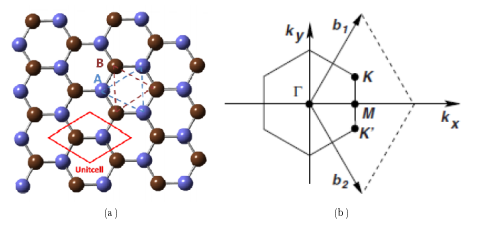
\includegraphics[width=0.7\linewidth]{../Figures/honeycomb_lattice.png}
  \caption{Image from a web source. In Fig. (a) the unit cell is sketched and the sublattices A and B are shown in blue and red respectively. In Fig. (b) the reciprocal lattice is shown, toghether with the high symmetry points $K$, $M$ and $K'$.} 
\label{Fig2.2}
\end{figure}
\end{section}
\end{subappendices}
 
\chapter{Perturbing the lattice}
\label{ChapPerturbing}

In this chapter we will derive an effective spin Hamiltonian for different models in the presence of a high frequency electromagnetic perturbation. The goal is to manipulate $J$ and $\bs{D}_{ij}$ in \ref{HeffNOEMF} separately. This has already been done for the case of Mott insulators (\cite{Mentink2015}, \cite{Kitamura2017}) where the starting Hamiltonian is the Hubbard model:

\begin{equation*}
\hat{H} = -t_0\sum_{\langle i,j \rangle, \sigma} \hat{c}_{i \sigma}^\dagger \hat{c}_{j \sigma} + \text{U} \sum_{i=1}^M \hat{n}_{i\uparrow}\hat{n}_{i\downarrow}
\end{equation*} 

In this model, since SOI is not taken into account, only the exchange interaction $J$ plays a role. The electromagnetic perturbation is then introduced via the Peierls substitution. We reproduce the result in section \ref{Section3Hubbard}. In the following sections we extend the analysis to different systems with spin orbit interaction thereby modulating $\bs{D}_{ij}$ or other spin interactions. The simplest model with spin orbit interaction is \ref{Hubbard}:

\begin{equation*}
\hat{H} = -\sum_{\langle i,j \rangle, \sigma, \sigma'}(\delta_{\sigma, \sigma'} t_{0} + \bs{\Delta}_{ij} \bs{\sigma}_{\sigma, \sigma'})\hat{c}_{i \sigma}^\dagger \hat{c}_{j \sigma'} + \text{U} \sum_{i=1}^M \hat{n}_{i\uparrow}\hat{n}_{i\downarrow}
\end{equation*}

Which is the same Hubbard model plus a spin dependent hopping term, which represents Rashba SOI for $\bs{\Delta}_{ij} = i\Delta_R(R_{ij}^y, -R_{ij}^x, 0)$ or Dresselhaus SOI for $\bs{\Delta}_{ij} = i\Delta_R(R_{ij}^x, -R_{ij}^y, 0)$. In section \ref{Section3HubbardSOI} we show how the exchange interaction and the DMI couplings are modulated in presence of an electromagnetic field.  

In the case of graphene or other coplanar honeycomb lattice structures, nearest neighbor Rashba terms are not allowed by symmetry, and only next nearest neighbor (NNN) spin conserving terms contribute \cite{Kane2005}, this term opens a gap in the band structure describing a topological insulator. For this case we examine the Kane-Mele-Hubbard model. The effective spin model of this Hamiltonian contains the usual exchange interaction and DMI and, in addition, it exhibits anisotropic exchange interaction arising from the intrinsic SOI term. This new term has already been obtained in \cite{Rachel2010} without taking into account any electromagnetic field.

Non-coplanar honeycomb lattice may exhibit intrinsic Rashba interactions between NNN \cite{Liu2011}, this, together with a NNN hopping (which would arise from direct overlapping of the next nearest neighbor Wannier functions or from second order processes) will lead to NNN DMI.


\begin{section}{Time dependent effective Hamiltonian}
\label{SectionTDHeff}

In this section we will derive a general effective Hamiltonian starting with any Hamiltonian that can be written as:

\begin{equation}
\hat{H} = -\hat{T} + \text{U}\hat{D}
\end{equation}
Where $\hat{D} = \sum_{i=1}^M \hat{n}_{i\uparrow}\hat{n}_{i\downarrow}$ is the doublon number operator and $\hat{T}$ is any hopping operator. In terms of on-site creation and annihilation operators we can write the hopping operator as $\hat{T} = \sum_{i,j, \sigma, \sigma'} t_{ij}^{\sigma \sigma'} \hat{c}_{i \sigma}^\dagger \hat{c}_{j \sigma'}$. The strength of the on-site interaction $\text{U}$ is much larger than the hopping amplitude, therefore, in a half filling system the zero double occupancies subspace $d=0$ can be taken as the low energy subspace in which the effective Hamiltonian will act.

The effect of the electromagnetic perturbation in the lattice can be introduced via the Peierls substitution (\ref{AP3A}). With this notation, in presence of a vector potential $\vec{A}(t)$ (which we assume to not vary noticeably in the scale of the lattice) the Peierls substitution leads to an extra time dependent phase in the hopping amplitude:

\begin{equation}
\label{TimeDepHopping}
t_{ij}^{\sigma \sigma'}(t) = t_{ij}^{\sigma \sigma'} e^{ie\bs{R}_{ij}\cdot\bs{A}(t)}
\end{equation}
Where $\bs{A}$ is the vector potential and $\bs{R}_{ij} = \bs{R}_i-\bs{R}_j$ and we take $\hbar=1$. We write the electric field as $\bs{E}(t) = \frac{1}{2}(\vec{E}e^{-i\omega t}+\vec{E}^*e^{i\omega t})$, where $\vec{E} = E_0\hat{e}$ and $\hat{e} = \frac{1}{\sqrt{1+\lambda_{POL}^2}}(\hat{e}_x+i\lambda_{POL}\hat{e}_y)$ is the polarization vector and $\lambda_{POL} = 0, \pm 1$ for plane polarized, right handed and left handed circular polarized field respectively. The vector potential takes the form $\bs{A}(t) = \frac{1}{2}(\vec{A}e^{-i\omega t} + \vec{A}^* e^{i\omega t})$, with $\vec{A} = \frac{iE_0}{\omega}\hat{e}$.
With the hopping amplitudes in \ref{TimeDepHopping} the Hamiltonian becomes time dependent. We will use Floquet theory \ref{APE} to derive an effective Hamiltonian including the laser perturbation.

Let us define:

\begin{equation}
\label{Def_alpha}
e\bs{R}_{ij}\vec{A} = \alpha_{ij} e^{i \theta_{ij}}
\end{equation}
With $\alpha_{ij} = \pm|e\bs{R}_{ij}\vec{A}|$ in such a way that:

\begin{align}
\alpha_{ij} &= -\alpha_{ji} \label{alphaSym} \\
\theta_{ij} &= \theta_{ji} \label{thetaSym}
\end{align}
and $\theta_{ij} \in \left[0,\pi\right)$. Then we can apply the Jacobi–Anger expansion:

\begin{align*}
t_{ij}^{\sigma \sigma'}(t) &= t_{ij}^{\sigma \sigma'}e^{ie\bs{R}_{ij}\cdot\bs{A}(t)} = t_{ij}^{\sigma \sigma'}e^{i\alpha_{ij} \cos(\omega t - \theta_{ij})} = \\
&= t_{ij}^{\sigma \sigma'}\sum_m e^{i(\frac{\pi}{2}-\theta_{ij})m} \mathcal{J}_m(\alpha_{ij}) e^{im\omega t} = \sum t_{ij,m}^{\sigma \sigma'} e^{im\omega t}
\end{align*}
Where we defined 

\begin{equation}
\label{HoppAmpFourier}
t_{ij,m}^{\sigma \sigma'} = t_{ij}^{\sigma \sigma'} e^{i(\frac{\pi}{2}-\theta_{ij})m} \mathcal{J}_m(\alpha_{ij})
\end{equation}
Which is the \textit{m}th Fourier mode of the hopping term and $\mathcal{J}_m(x)$ is the \textit{m}th Bessel function \cite{Kitamura2017}. Correspondingly we can write $\hat{T}(t) = \sum_m \hat{T}_m e^{im \omega t}$ where $\hat{T}_m$ is the sum of all the \textit{m}th Fourier mode of the hopping terms. We can further decompose the hopping operator into:

\begin{equation}
\hat{T}(t) = \sum_m (\hat{T}_{-1,m}+\hat{T}_{0,m}+\hat{T}_{1,m})e^{im\omega t}
\end{equation}
Where $\hat{T}_{dm}(t)$ changes the doublon number by $d$, for example, if $\hat{P}_d$ is the projection operator into the subspace with doublon number $d$, then $\hat{T}_{dm}(t) = \sum_i \hat{P}_{i+d}\hat{T}_{m}(t)\hat{P}_i$. Since the hopping term is of second order in the creation and annihilation operators, it can change the double occupancy of the states only by $\pm1$.

In order to derive the form of the effective spin Hamiltonian let us introduce a time dependent unitary transformation $\hat{U}(t) = e^{-i\hat{S}(t)}$. The transformed Hamiltonian is:

\begin{equation}
\hat{H}'(t) = e^{i\hat{S}(t)} \hat{H}(t) e^{-i\hat{S}(t)} - e^{i\hat{S}(t)} id_t e^{-i\hat{S}(t)}
\end{equation} 
We perform the unitary transformation perturbatively in the hopping operator, we can formally write $\hat{T}(t) = \eta \hat{T}(t)$, where $\eta$ will play the role of a bookkeeping parameter in the perturbative expansion. We expand $\hat{S}(t) = \sum_\nu \eta^\nu \hat{S}^{(\nu)}(t)$ and $\hat{H}'(t) = \sum_\nu \eta^\nu \hat{H}'^{(\nu)}(t)$. We require the transformed Hamiltonian to be block diagonal in the doublon number operator $\hat{d}$. To fulfill this requirement, the unitary transformation $\hat{S}(t)$ must have the same periodicity as $\hat{T}(t)$; consequently, the transformed Hamiltonian $\hat{H}'(t)$ will have the same periodicity as the original Hamiltonian $\hat{H}(t)$. Thus we can write $\hat{S}^{(\nu)}(t) = \sum_m e^{im\omega t}\hat{S}^{(\nu)}_m$. With the further requirement that $\hat{S}(t)$ does not contain block-diagonal terms, we can uniquely determine the unitary transformation:

\begin{equation}
\hat{S}^{(\nu)}(t) = \sum_{d \neq 0} \sum_m \eta^\nu \hat{S}^{(\nu)}_{d,m} e^{im\omega t}
\end{equation}
where $\hat{S}^{(\nu)}_{d,m}$ changes the double occupancy number by $d$.

Now we can use the identity:

\begin{equation}
id_t e^{-i\hat{S}(t)} = \sum_n \frac{1}{(n+1)!}\text{ad}_{-i\hat{S}(t)}^n (d_t \hat{S}(t))e^{-i\hat{S}(t)}
\end{equation}
Derived in appendix \ref{AP3B}, where $\text{ad}_A(B) = [A,B]$ to rewrite the transformed Hamiltonian as:

\begin{equation}
\hat{H}'(t) = e^{i\hat{S}(t)} \left( \hat{H}(t) - \sum_n \frac{1}{(n+1)!}\text{ad}_{-i\hat{S}(t)}^n (d_t \hat{S}(t)) \right) e^{-i\hat{S}(t)}
\end{equation}
Using the Baker–Campbell–Hausdorff expansion we can write the transformed Hamiltonian as:

\begin{equation}
\label{PertFull}
\hat{H}'(t) = \sum_m \frac{1}{m!} \text{ad}_{i\hat{S}(t)}^m \left( \hat{H}(t) - \sum_n \frac{1}{(n+1)!}\text{ad}_{-i\hat{S}(t)}^n (d_t \hat{S}(t)) \right)
\end{equation}
Now, in this expression we have to expand $\hat{S}(t) = \sum_\nu \eta^\nu \hat{S}^{(\nu)}(t)$ and $\hat{H}'(t) = \sum_\nu \eta^\nu \hat{H}'^{(\nu)}(t)$ and determine $\hat{S}^{(\nu)}(t)$ iteratively in $\nu$ so that $\hat{H}'^{(\nu)}(t)$ is diagonal in the doublon number. Notice that we do not expand $\hat{H}(t)$ as an infinite series since $\hat{H}(t) = -\eta \hat{T}(t) + \text{U}\hat{D}$. Now, notice also that if we take $i\hat{S}^{(0)}(t)=0$ in \ref{PertFull}, then, to zeroth order in $\eta$ only terms in $m=0$ and $n=0$ contribute obtaining:

\begin{equation}
\hat{H}'^{(0)}(t) = \text{U}\hat{D}
\end{equation}
Which is indeed diagonal in the doublon number, and therefore we can take $i\hat{S}^{(0)}(t)=0$. With this equating terms of the same order in \ref{PertFull} is greatly simplified, since terms with high $m,n$ will correspond to terms with high $\eta$. Since we are only interested in orders up to second order, we can truncate \ref{PertFull} up to $m=2$:

\begin{align}
\label{PertTrunc}
\hat{H}'(t) &=  \hat{H}(t) - \sum_n \frac{1}{(n+1)!}\text{ad}_{-i\hat{S}(t)}^n (d_t \hat{S}(t)) + [i\hat{S}(t), \hat{H}(t) - \sum_n \frac{1}{(n+1)!}\text{ad}_{-i\hat{S}(t)}^n (d_t \hat{S}(t))] + \nonumber \\
&+ \frac{1}{2} [i\hat{S}(t),[i\hat{S}(t), \hat{H}(t) - \sum_n \frac{1}{(n+1)!}\text{ad}_{-i\hat{S}(t)}^n (d_t \hat{S}(t)) ]]
\end{align}
This equation holds up to order $\eta^2$. In first order we obtain:

\begin{equation}
\label{1stO}
\hat{H}'^{(1)}(t) = -\hat{T}(t) - d_t\hat{S}^{(1)}(t) + \left[ i\hat{S}^{(1)}(t), \text{U}\hat{D} \right]
\end{equation}
Now we expanding in $m,d$ and use $\left[ \hat{D}, \hat{S}^{(\nu)}_{dm} \right] = d\hat{S}^{(\nu)}_{dm}$ because $\hat{S}^{(\nu)}_{dm}$ changes the doublon number by $d$:

\begin{equation}
\hat{H}'^{(1)}(t)=-\hat{T}(t)-\sum_{d\neq 0}\sum_m (\text{U}d+m\omega) i\hat{S}^{(1)}_{dm} e^{im\omega t}
\end{equation}
Therefore:

\begin{align}
i\hat{S}^{(1)}_d(t) &= -\sum_m \frac{\hat{T}_{d,m}}{\text{U}d+m\omega}e^{im\omega t} \label{1stOSpin}\\
\hat{H}'^{(1)}(t) &= -\sum_m \hat{T}_{0,m}(t)e^{im\omega t} \label{1stOH}
\end{align}
To second order we find:

\begin{align}
\hat{H}'^{(2)}(t) &= - d_t\hat{S}^{(2)}(t) - \frac{1}{2}\left[-i\hat{S}^{(1)}(t), d_t\hat{S}^{(1)}(t) \right] + \left[i\hat{S}^{(1)}(t), -\hat{T}(t)-\frac{1}{2}d_t\hat{S}^{(1)}(t) \right] +\nonumber \\
&+ \left[i\hat{S}^{(2)}(t), \text{U}\hat{D} \right] + \frac{1}{2} \left[i\hat{S}^{(1)}(t), \left[i\hat{S}^{(1)}(t), \text{U}\hat{D} \right] \right] = \nonumber \\
&= \left[i\hat{S}^{(2)}(t), \text{U} \hat{D} \right] - \left[ i\hat{S}^{(1)}(t), \hat{T}(t) \right] + \frac{1}{2}\left[ i\hat{S}^{(1)}(t), \left[ i\hat{S}^{(1)}(t), \text{U}\hat{D} \right] \right] - d_t\hat{S}^{(2)}(t)
\end{align}
Using \ref{1stO} and using $\left[ i\hat{S}^{(1)}(t), d_t\hat{S}^{(1)}(t)\right] = 0$ due to different Fourier modes of the hopping operator being equal up to a constant (explain better), we can rewrite:

\begin{equation}
\hat{H}'^{(2)}(t) = \left[i\hat{S}^{(2)}(t), \text{U} \hat{D} \right] - \frac{1}{2}\left[ i\hat{S}^{(1)}(t), \hat{T}(t) - \hat{H}'^{(1)}(t)\right] - d_t\hat{S}^{(2)}(t)
\end{equation}
Using \ref{1stOSpin} and \ref{1stOH}, the middle term is:

\begin{align*}
&\left[ i\hat{S}^{(1)}(t), \hat{T}(t) - \hat{H}'^{(1)}(t)\right] = -\left[\sum_m \left( \frac{\hat{T}_{1m}}{\text{U}+m\omega} - \frac{\hat{T}_{-1m}}{\text{U}-m\omega} \right)e^{im \omega t}, \sum_n \left( \hat{T}_{-1n} + 2\hat{T}_{0n} + \hat{T}_{1n} \right) e^{in\omega t} \right] \\
&= -\sum_{mn} \left\{ \frac{2\left[\hat{T}_{1m}, \hat{T}_{0n} \right]}{\text{U}+m\omega} + \frac{\left[\hat{T}_{1m}, \hat{T}_{-1n} \right]}{\text{U}+m\omega} - \frac{\left[\hat{T}_{-1m}, \hat{T}_{1n} \right]}{\text{U}-m\omega} - \frac{2\left[\hat{T}_{-1m}, \hat{T}_{0n} \right]}{\text{U}-m\omega} \right\} e^{i(m+n)\omega t} \\
&= -\sum_{mn} \left\{ \frac{2\left[\hat{T}_{1n}, \hat{T}_{0(m-n)} \right]}{\text{U}+n\omega} + \frac{\left[\hat{T}_{1n}, \hat{T}_{-1(m-n)} \right]}{\text{U}+n\omega} - \frac{\left[\hat{T}_{-1n}, \hat{T}_{1(m-n)} \right]}{\text{U}-n\omega} - \frac{2\left[\hat{T}_{-1n}, \hat{T}_{0(m-n)} \right]}{\text{U}-n\omega} \right\} e^{im\omega t}
\end{align*}
Altogether:

\begin{align*}
\hat{H}'^{(2)}(t) &= \sum_{mn} \left\{ \frac{\left[\hat{T}_{1n}, \hat{T}_{0(m-n)} \right]}{\text{U}+n\omega} + \frac{\left[\hat{T}_{1n}, \hat{T}_{-1(m-n)} \right]}{2(\text{U}+n\omega)} - \frac{\left[\hat{T}_{-1n}, \hat{T}_{1(m-n)} \right]}{2(\text{U}-n\omega)} - \frac{\left[\hat{T}_{-1n}, \hat{T}_{0(m-n)} \right]}{\text{U}-n\omega} \right\} e^{im\omega t} \\
&-\sum_{d\neq 0}\sum_m (\text{U}d+m\omega) i\hat{S}^{(2)}_{dm} e^{im\omega t}
\end{align*}
By choosing $i\hat{S}^{(2)}_{dm}$ such that the transformed Hamiltonian is block-diagonal, we obtain:

\begin{align}
i\hat{S}^{(2)}_{dm} &= \sum_n \frac{\left[ \hat{T}_{dn}, \hat{T}_{0(m-n)} \right]}{(\text{U}d+n\omega)(\text{U}d+m\omega)} \label{2ndOSpin}\\
\hat{H}'^{(2)}(t) &= \frac{1}{2}\sum_{mn} \left( \frac{\left[\hat{T}_{1n}, \hat{T}_{-1(m-n)} \right]}{\text{U}+n\omega} - \frac{\left[\hat{T}_{-1n}, \hat{T}_{1(m-n)} \right]}{\text{U}-n\omega} \right) e^{im\omega t} \label{2ndOH}
\end{align}
Now the effective Hamiltonian acts on the subspace of $d=0$ (zero double occupancies), therefore we are only interested on the block $\hat{P}_0 \hat{H}'^{(2)}(t) \hat{P}_0$ (notice that $\hat{P}_0 \hat{H}'^{(1)}(t) \hat{P}_0 = 0$). In this subspace we can write:

\begin{align}
\hat{H}_{\text{eff}}(t) &= \hat{P}_0\hat{H}'^{(2)}(t)\hat{P}_0 = -\frac{1}{2}\sum_{mn} \left( \frac{\hat{P}_0  \hat{T}_{-1(m-n)}\hat{T}_{1n}\hat{P}_0}{\text{U}+n\omega} + \frac{\hat{P}_0 \hat{T}_{-1n} \hat{T}_{1(m-n)} \hat{P}_0}{\text{U}-n\omega} \right) e^{im\omega t} \nonumber \\
&= -\frac{1}{2}\sum_{mn} \left\{ \frac{\hat{P}_0  (\hat{T}_{-1(m-n)}\hat{T}_{1n} + \hat{T}_{-1-n}\hat{T}_{1(m+n)})\hat{P}_0}{\text{U}+n\omega} \right\} e^{im\omega t} \label{2ndOHeff}
\end{align}
Now, since the hopping operators act on the subspace $d=0$ and must remain within that subspace, therefore $\hat{P}_0 \hat{T}_{-1a} \hat{T}_{1b} \hat{P}_0$ will be a sum of all possible hoppings between two different sites:

\begin{align*}
\hat{P}_0 \hat{T}_{-1a} \hat{T}_{1b} \hat{P}_0 = \sum_{i,j, \sigma_1, \sigma_2, \sigma_3, \sigma_4} t_{ij,a}^{\sigma_1 \sigma_2} t_{ji,b}^{\sigma_3 \sigma_4} \hat{c}_{i \sigma_1}^\dagger \hat{c}_{j \sigma_2} \hat{c}_{j \sigma_3}^\dagger \hat{c}_{i \sigma_4}
\end{align*}
Where $a$ and $b$ are any two Fourier modes. Inserting this into \ref{HeffSimplified} and using the definition of $t_{ij,m}^{\sigma \sigma'} = t_{ij}^{\sigma \sigma'} e^{i(\frac{\pi}{2}-\theta_{ij})m} \mathcal{J}_m(\alpha_{ij})$ and using that $\theta_{ji} = \theta_{ij}$ and $\alpha_{ji} = -\alpha_{ij}$ and the properties $\mathcal{J}_{-m}(x) = (-1)^m\mathcal{J}_m(x)$ and $\mathcal{J}_m(-x) = (-1)^m\mathcal{J}_m(x)$ we can write \ref{HeffSimplified} as:

\begin{align}
&\hat{H}_{\text{eff}}(t) = \hat{P}_0\hat{H}'^{(2)}(t)\hat{P}_0 = - \frac{1}{2}\sum_{mn} \sum_{i,j, \sigma_1, \sigma_2, \sigma_3, \sigma_4}\hat{c}_{i \sigma_1}^\dagger \hat{c}_{j \sigma_2} \hat{c}_{j \sigma_3}^\dagger \hat{c}_{i \sigma_4} \frac{t_{ij,m-n}^{\sigma_1 \sigma_2} t_{ji,n}^{\sigma_3 \sigma_4} + t_{ij,-n}^{\sigma_1 \sigma_2} t_{ji,m+n}^{\sigma_3 \sigma_4}}{\text{U}+n\omega} e^{im\omega t} \nonumber \\
&= - \frac{1}{2}\sum_{mn} \sum_{i,j, \sigma_1, \sigma_2, \sigma_3, \sigma_4} \left\{ \hat{c}_{i \sigma_1}^\dagger \hat{c}_{j \sigma_2} \hat{c}_{j \sigma_3}^\dagger \hat{c}_{i \sigma_4} t_{ij}^{\sigma_1 \sigma_2} t_{ji}^{\sigma_3 \sigma_4} e^{i(\frac{\pi}{2}-\theta_{ij})m} \right. \nonumber \\
& \left. \frac{ \mathcal{J}_{m-n}(\alpha_{ij}) \mathcal{J}_{n}(\alpha_{ji}) + \mathcal{J}_{-n}(\alpha_{ij}) \mathcal{J}_{m+n}(\alpha_{ji})}{\text{U}+n\omega} e^{im\omega t} \right\} \nonumber \\
&= - \frac{1}{2}\sum_{mn} \sum_{i,j, \sigma_1, \sigma_2, \sigma_3, \sigma_4} \left\{ \hat{c}_{i \sigma_1}^\dagger \hat{c}_{j \sigma_2} \hat{c}_{j \sigma_3}^\dagger \hat{c}_{i \sigma_4} t_{ij}^{\sigma_1 \sigma_2} t_{ji}^{\sigma_3 \sigma_4} e^{i(\frac{\pi}{2}-\theta_{ij})m} (-1)^m \right. \nonumber \\
&\left. \frac{ \mathcal{J}_{n-m}(\alpha_{ij}) \mathcal{J}_{n}(\alpha_{ij}) + \mathcal{J}_{n}(\alpha_{ij}) \mathcal{J}_{m+n}(\alpha_{ij})}{\text{U}+n\omega} e^{im\omega t} \right\} \nonumber \\
&= - \frac{1}{2} \sum_{i,j, \sigma_1, \sigma_2, \sigma_3, \sigma_4}\hat{c}_{i \sigma_1}^\dagger \hat{c}_{j \sigma_2} \hat{c}_{j \sigma_3}^\dagger \hat{c}_{i \sigma_4} t_{ij}^{\sigma_1 \sigma_2} t_{ji}^{\sigma_3 \sigma_4} \mathcal{M}(\alpha_{ij}, \text{U}, \omega, t) \label{HeffSimplified}
\end{align}
Where we defined:

\begin{equation}
\mathcal{M}(\alpha_{ij}, \text{U}, \omega, t) = \sum_{mn}e^{-i(\frac{\pi}{2}+\theta_{ij})m} \left\{ 
    \frac{\mathcal{J}_{n-m}(\alpha_{ij})\mathcal{J}_{n}(\alpha_{ij}) + \mathcal{J}_{n}(\alpha_{ij})\mathcal{J}_{m+n}(\alpha_{ij})}{\text{U}+n\omega} \right\}e^{im\omega t}
\end{equation}
In the following sections we will use this effective Hamiltonian for different models of the hopping operator. In each case we will introduce the spin relations \ref{SpinOperatorInv1} and \ref{SpinOperatorInv2} together with \ref{SpinRel1}, \ref{SpinRel2} and \ref{SpinRel3} to obtain the corresponding effective spin Hamiltonian. 

\begin{subsection}{Time independent field}

Before we start using \ref{HeffSimplified} for different models we would like to investigate the case in which the electric field is time independent. In that case we can restrict the analysis to the one dimensional lattice, since in second order the electric field will only affect the bonds parallel to the field. Let us denote $\vec{\bs{E}} = E_0 \hat{e}_x$, then the Peiels transformed hopping amplitudes can be written as:

\begin{equation}
\label{TimeIndepHoppingAmpl}
t_{ij}^{\sigma \sigma'} (t) = t_{ij}^{\sigma \sigma'} e^{ie \vec{\bs{R}}_{ij} \cdot \vec{\bs{E}} t}
\end{equation}
Therefore, there will be only two Fourier modes with frequency $\omega_0 = e \vec{\bs{R}}_{ij} \cdot \vec{\bs{E}} = \pm eaE_0$, where the sign $+(-)$ corresponds to the case $\vec{\bs{R}}_{ij} = \pm a \hat{e}_x$. Notice that this frequency $\omega_0$ does not correspond to a field frequency ($\vec{\bs{E}}$ is time independent), but to the Fourier mode in the hopping amplitudes (which is induced by the time independent field). From this point we can apply the same procedure as in the general case up to \ref{2ndOHeff}. We can greatly simplify this by considering that:
\begin{itemize}
	\item $n$ can only take values $ n = \pm 1$ (there are no additional Fourier modes).
	\item When restricted to the low energy subspace a product $\hat{T}_{-1 a} \hat{T}_{1 b}$ will only contribute when $a$ and $b$ have opposite signs ($a=1, b=-1$ or viceversa). This is because, in the low energy subspace $\hat{T}_{-1 a} \hat{T}_{1 b}$ can only represent a hopping from a site $i$ to a site $j$ and the hopping back to $i$, we can see from \ref{TimeIndepHoppingAmpl} that these two amplitudes will be in opposite Fourier modes.
\end{itemize}
Taking this into consideration we see that only $m=0$ terms will remain, which is consistent with the fact that the two phases cancel out in the process $i \rightarrow j \rightarrow i$. We can thus rewrite \ref{2ndOHeff} as:

\begin{equation}
\hat{H}_{\text{eff}} = -\hat{P}_0 \left\{ \frac{\hat{T}_{-1,1}\hat{T}_{1,-1} }{\text{U}-\omega_0} + \frac{\hat{T}_{-1,-1}\hat{T}_{1,1} }{\text{U}+\omega_0} \right\} \hat{P}_0
\end{equation}
Now, the first fraction represents a hopping process $i\rightarrow j \rightarrow i$ where $j$ lies left to $i$, whereas in the second fraction $j$ lies right to $i$:

\begin{align*}
\hat{P}_0 \hat{T}_{-1,1} \hat{T}_{1,-1} \hat{P}_0 &= \sum_{i > j, \sigma_1, \sigma_2, \sigma_3, \sigma_4} t_{ij}^{\sigma_1 \sigma_2} t_{ji}^{\sigma_3 \sigma_4} \hat{c}_{i \sigma_1}^\dagger \hat{c}_{j \sigma_2} \hat{c}_{j \sigma_3}^\dagger \hat{c}_{i \sigma_4} \\
\hat{P}_0 \hat{T}_{-1,-1} \hat{T}_{1,1} \hat{P}_0 &= \sum_{i < j, \sigma_1, \sigma_2, \sigma_3, \sigma_4} t_{ij}^{\sigma_1 \sigma_2} t_{ji}^{\sigma_3 \sigma_4} \hat{c}_{i \sigma_1}^\dagger \hat{c}_{j \sigma_2} \hat{c}_{j \sigma_3}^\dagger \hat{c}_{i \sigma_4} 
\end{align*}
We can rewrite this in the more compact form:

\begin{equation}
\label{TimeIndepHeff}
\hat{H}_{\text{eff}} = -\sum_{i, j, \sigma_1, \sigma_2, \sigma_3, \sigma_4} \frac{t_{ij}^{\sigma_1 \sigma_2} t_{ji}^{\sigma_3 \sigma_4} \hat{c}_{i \sigma_1}^\dagger \hat{c}_{j \sigma_2} \hat{c}_{j \sigma_3}^\dagger \hat{c}_{i \sigma_4}}{\text{U} + \text{sgn}(j-i)\omega_0}
\end{equation}
This is the same effective Hamiltonian obtained in the previous section without an electric field but with a shift in the intermediate state energy by $\pm \omega_0 = \pm eaE_0$. We will analyze the corresponding spin Hamiltonian of this effective Hamiltonian when we consider the Kane-Mele-Hubbard model in Section \ref{section3NNN}.

\end{subsection}

\end{section}


\begin{section}{Hubbard model without SOI}
\label{Section3Hubbard}
We start by considering the simplest hopping operator, excluding SOI terms \ref{HnoSOI}:

\begin{equation}
\hat{H} = -t_0\sum_{\langle i,j \rangle, \sigma} \hat{c}_{i \sigma}^\dagger \hat{c}_{j \sigma} + \text{U} \sum_{i=1}^M \hat{n}_{i\uparrow}\hat{n}_{i\downarrow}
\end{equation}

We see that the hopping amplitudes introduced in the previous section can be written as $t_{ij}^{\sigma \sigma'} = \delta_{\sigma \sigma'} t_0$ for $i,j$ being nearest neighbors, and $t_{ij}^{\sigma \sigma'} = 0$ otherwise. With this we can directly apply \ref{HeffSimplified} to obtain:

\begin{equation}
\hat{H}_{\text{eff}}(t) = -\frac{t_0^2}{2} \sum_{\langle i,j \rangle, \sigma, \sigma'} \hat{c}_{i \sigma}^\dagger \hat{c}_{j \sigma} \hat{c}_{j \sigma'}^\dagger \hat{c}_{i \sigma'} \mathcal{M}(\alpha_{ij}, \text{U}, \omega, t)
\end{equation}

Now, introducing the spin operators \ref{SpinOperatorInv1} and \ref{SpinOperatorInv2} and summing over the spin states as in \ref{SpinRel1}:

\begin{align*}
\sum_{\sigma, \sigma'} \hat{c}_{i \sigma}^\dagger \hat{c}_{j \sigma} \hat{c}_{j \sigma'}^\dagger \hat{c}_{i \sigma'} = \sum_{\sigma, \sigma'} \left( \frac{\delta_{\sigma \sigma'}}{2} + \bs{S}_i\cdot\bs{\sigma}_{\sigma' \sigma} \right) \left( \frac{\delta_{\sigma \sigma'}}{2} - \bs{S}_j\cdot\bs{\sigma}_{\sigma \sigma'} \right) = -2\bs{S}_i\cdot \bs{S}_j
\end{align*}

Where we neglected the constant term. The effective spin Hamiltonian is thus:

\begin{equation}
\hat{H}_{\text{eff}}(t) = \sum_{\langle i,j \rangle} J_{ij} \bs{S}_i \cdot \bs{S}_j
\end{equation}

With 

\begin{align}
J_{ij} &= t_0^2 \mathcal{M}(\alpha_{ij}, \text{U}, \omega, t) \nonumber \\
&=\sum_{mn} t_0^2 e^{-i(\frac{\pi}{2}+\theta_{ij})m}\left(\frac{\mathcal{J}_{n-m}(\alpha_{ij})\mathcal{J}_{n}(\alpha_{ij})+\mathcal{J}_{n}(\alpha_{ij})\mathcal{J}_{n+m}(\alpha_{ij})}{\text{U}+n\omega} \right) e^{im\omega t} \label{Jij1}
\end{align}

After time average this reduces to the $m=0$ term:

\begin{equation}
\label{MFactorApprox0}
\mathcal{M}(\alpha_{ij}, \text{U}, \omega) \approx \sum_{n} 2 \frac{\mathcal{J}_n(\alpha_{ij})^2}{\text{U}+n\omega}
\end{equation}

For $\omega>>U$ we can truncate this to the three smallest values of $n$, i.e. $n=0, \pm 1$. We can also use that $\alpha_{ij} << 1$ because $\alpha_{ij}$ is proportional to $\vec{A}$ which is proportional to $\omega^{-1}$. Therefore we can use $\mathcal{J}_n(x) \approx x^n \text{ for } n>0 \text{ and } x << 1$ to obtain:

\begin{equation}
\label{MFactorApprox}
\mathcal{M}(\alpha_{ij}, \text{U}, \omega) \approx 2 \left(\frac{\alpha_{ij}^2}{\text{U}+\omega} +\frac{1}{\text{U}} +\frac{\alpha_{ij}^2}{\text{U}-\omega} \right)
\end{equation}

And the exchange interaction coupling becomes:

\begin{equation}
\label{Jij2}
J_{ij} \approx J_{ij}^0 + 2t_0^2 \alpha_{ij}^2 \left( \frac{1}{\text{U}+\omega} + \frac{1}{\text{U}-\omega} \right)
\end{equation}

The lattice structure is contained in $\alpha_{ij} = \pm|e\bs{R}_{ij}\vec{A}|$. For a square lattices aligned with the coordinate system so that $\vec{a}_1=\hat{e}_x$ and $\vec{a}_2=\hat{e}_y$, we will have $\bs{R}_{ij} = \pm a\hat{e}_x,\pm a\hat{e}_y$, where $a$ is the lattice constant. Using $\vec{A}=\frac{iE_0}{\omega\sqrt{1+\lambda^2}}(\hat{e}_x+i\lambda\hat{e}_y)$ we have:

\begin{equation}
\alpha_{ij} = \begin{cases}
             \pm \frac{eaE_0}{\omega \sqrt{1+\lambda^2}} = \pm \frac{\mathcal{E}}{\sqrt{1+\lambda^2}},  & \text{for } \bs{R}_{ij} = \pm \hat{e}_x \\
             \pm \lambda\frac{eaE_0}{\omega \sqrt{1+\lambda^2}} = \pm \frac{\lambda \mathcal{E}}{\sqrt{1+\lambda^2}},  & \text{for } \bs{R}_{ij} = \pm \hat{e}_y
       \end{cases} \quad
\end{equation}

Where $\mathcal{E} = \frac{eaE_0}{\omega}$. 

For plane polarized light ($\lambda = 0$) the exchange interaction only changes in the direction of the polarization, that is:

\begin{equation}
J_{ij}^{PP} = \begin{cases}
		J_{ij}^0 + 2t_0^2 \mathcal{E}^2 \left( \frac{1}{\text{U}+\omega} + \frac{1}{\text{U}-\omega} \right) & \text{for } \bs{R}_{ij} = \pm \hat{e}_x \\
J_{ij}^0 & \text{for } \bs{R}_{ij} = \pm \hat{e}_y
\end{cases} \quad 
\end{equation}

For circular polarized light ($\lambda=\pm1$) in this approximation the exchange interaction changes in the same way in all the directions:

\begin{equation}
\label{JijCPSQUARE}
J_{ij}^{CP} = J_{ij}^0 + t_0^2 \mathcal{E}^2 \left( \frac{1}{\text{U}+\omega} + \frac{1}{\text{U}-\omega} \right)
\end{equation}

Notice that this result is independent of the helicity of the applied field, this is true even if we do not make the approximation \ref{MFactorApprox}. 

\begin{subsection}{Honeycomb lattice}

Now consider a honeycomb lattice structure, so that the $\alpha_{ij}$ values are given by $\alpha_{ij} = \pm|e\bs{R}_{ij}\vec{A}|$ where $\bs{R}_{ij}$ are the displacement vectors in a honeycomb lattice. There are six such vectors:

\begin{align}
\bs{R}_1^\pm &= \pm a\hat{e}_x \\
\bs{R}_2^\pm &= \pm a\frac{1}{2}(\hat{e}_x + \sqrt{3}\hat{e}_y) \\
\bs{R}_3^\pm &= \pm a\frac{1}{2}(\hat{e}_x - \sqrt{3}\hat{e}_y)
\end{align}

These six possible directions will lead to $\alpha_a^\pm = \pm |e\bs{R}_a\vec{A}|$ where $\vec{A}=\frac{iE_0}{\omega\sqrt{1+\lambda^2}}(\hat{e}_x+i\lambda\hat{e}_y)$:

\begin{align}
\alpha_1^\pm &= \pm \frac{eaE_0}{\omega\sqrt{1+\lambda^2}} \\
\alpha_2^\pm &= \alpha_3^\pm = \pm \frac{eaE_0}{2\omega} \sqrt{\frac{1+3\lambda^2}{1+\lambda^2}} = \pm\frac{eaE_0}{2\omega}\sqrt{1+\frac{2\lambda^2}{1+\lambda^2}}
\end{align}

From here we can see that if we take the same approximation as in \ref{Jij2} we will obtain the same form of exchange interaction for circular polarized light ($\lambda=\pm1$) \ref{JijCPSQUARE} with possibly a different lattice constant $a$. 

\end{subsection}

\begin{subsection}{Dielectric permittivity}

Using the approximation for the exchange coupling constant for circular polarized light derived in \ref{JijCPSQUARE} we can write the free energy of the system $\Phi$ as:

\begin{align}
\Phi &= \Phi_0 + \sum_{\langle i,j \rangle} J_{ij} \bs{S}_i \cdot \bs{S}_j = \nonumber \\
&= \Phi_0 + \sum_{\langle i,j \rangle} J_{ij}^0 \bs{S}_i \cdot \bs{S}_j + |\vec{E}_0|^2 \frac{t_0^2 e^2 a^2}{\omega}\left( \frac{1}{\text{U}+\omega} + \frac{1}{\text{U}-\omega} \right)\sum_{\langle i,j \rangle} \bs{S}_i \cdot \bs{S}_j
\end{align}

Then, the dielectric permittivity is $\epsilon_{kl} = \frac{\partial^2 \Phi}{\partial E_k \partial E_l}$, i.e., the dielectric permittivity is isotropic $\epsilon_{kl} = \epsilon$ and:

\begin{equation}
\epsilon = \epsilon^0 + 2\frac{t_0^2 e^2 a^2}{\omega}\left( \frac{1}{\text{U}+\omega} + \frac{1}{\text{U}-\omega} \right)\sum_{\langle i,j \rangle} \bs{S}_i \cdot \bs{S}_j
\end{equation}

Where $\epsilon^0 = \frac{\partial^2 \Phi_0}{\partial E_k \partial E_l}$. The refractive index will therefore depend on the magnetization of the antiferromagnet, this was already demonstrated experimentally in the 80's \cite{Demokritov1985}.
\end{subsection}

\end{section}

\begin{section}{Hubbard model with SOI}
\label{Section3HubbardSOI}
Now, let's investigate the effect of the electric field for the Hubbard model with SOI, i.e. \ref{Hubbard}, in this case the hopping operator gets an extra spin-dependent term:

\begin{equation}
\hat{T} = \sum_{\langle i,j \rangle, \sigma, \sigma'}(\delta_{\sigma, \sigma'} t_0 + \bs{\Delta}_{ij} \cdot \bs{\sigma}_{\sigma, \sigma'})\hat{c}_{i \sigma}^\dagger \hat{c}_{j \sigma'}
\end{equation}
The vector $\bs{\Delta}_{ij}$ can describe Rashba or Dresselhaus SOI, $\bs{\Delta}_{ij} = i\Delta_R(R_{ij}^y, -R_{ij}^x, 0)$ for Rashba SOI and $\bs{\Delta}_{ij} = i\Delta_R(R_{ij}^x, -R_{ij}^y, 0)$ for Dresselhaus SOI. 
In this case the hopping amplitudes are:

\begin{equation}
\label{HoppHubbSOI}
t_{ij}^{\sigma \sigma'} = \begin{cases}
	(\delta_{\sigma \sigma'}t_0+\bs{\Delta}_{ij} \cdot \bs{\sigma}_{\sigma, \sigma'}) & \text{for } i, j \text{ nearest neighbors} \\
	0 & \text{ otherwise}
\end{cases} \quad
\end{equation}

And as before $\hat{H} = -\hat{T} + \text{U}\hat{D}$. In the presence of an electromagnetic field we can apply the Peierls substitution as we did before, and the effective Hamiltonian will be given by \ref{HeffSimplified}.  inserting the spin operators \ref{SpinOperatorInv1} and \ref{SpinOperatorInv2} we get:

\begin{align}
\hat{H}_{\text{eff}}(t) &= - \frac{1}{2} \sum_{\langle i,j \rangle, \sigma_1, \sigma_2, \sigma_3, \sigma_4}\hat{c}_{i \sigma_1}^\dagger \hat{c}_{j \sigma_2} \hat{c}_{j \sigma_3}^\dagger \hat{c}_{i \sigma_4} t_{ij}^{\sigma_1 \sigma_2} t_{ji}^{\sigma_3 \sigma_4} \mathcal{M}(\alpha_{ij}, \text{U}, \omega, t) \nonumber \\
&= - \frac{1}{2} \sum_{\langle i,j \rangle, \sigma_1, \sigma_2, \sigma_3, \sigma_4} \left( \frac{\delta_{\sigma_1 \sigma_4}}{2} + \bs{S}_i\cdot\bs{\sigma}_{\sigma_4 \sigma_1} \right) \left( \frac{\delta_{\sigma_2 \sigma_3}}{2} - \bs{S}_j\cdot\bs{\sigma}_{\sigma_2 \sigma_3} \right) \nonumber \\ &(\delta_{\sigma_1 \sigma_2}t_0+\bs{\Delta}_{ij}\cdot \bs{\sigma}_{\sigma_1, \sigma_2}) (\delta_{\sigma_3 \sigma_4}t_0+\bs{\Delta}_{ji}\cdot \bs{\sigma}_{\sigma_3, \sigma_4}) \mathcal{M}(\alpha_{ij}, \text{U}, \omega, t) \label{HeffHubbSOI1}
\end{align}
Using $\bs{\Delta}_{ji} = - \bs{\Delta}_{ij}$:

\begin{align*}
&(\delta_{\sigma_1 \sigma_2}t_0+\bs{\Delta}_{ij} \cdot\bs{\sigma}_{\sigma_1, \sigma_2}) (\delta_{\sigma_3 \sigma_4}t_0+\bs{\Delta}_{ji}\cdot \bs{\sigma}_{\sigma_3, \sigma_4}) = \\ 
&\delta_{\sigma_1 \sigma_2}\delta_{\sigma_3 \sigma_4}t_0^2 + t_0\bs{\Delta}_{ij}\cdot(\delta_{\sigma_3 \sigma_4} \bs{\sigma}_{\sigma_1 \sigma_2} - \delta_{\sigma_1 \sigma_2} \bs{\sigma}_{\sigma_3 \sigma_4}) - (\bs{\Delta}_{ij}\cdot\bs{\sigma}_{\sigma_1, \sigma_2})(\bs{\Delta}_{ij}\cdot\bs{\sigma}_{\sigma_3, \sigma_4})
\end{align*}
The term proportional to $t_0^2$ will lead to the modified exchange interaction, as in the previous section. The term proportional to $t_0\bs{\Delta}_{ij}$ will lead to the modified DMI interaction and the term proportional to $\bs{\Delta}_{ij}^2$ will lead to the pseudodipolar interaction.

Now we can rewrite \ref{HeffHubbSOI1} as:

\begin{align*}
\hat{H}_{\text{eff}}(t) &= - \frac{1}{2} \sum_{\langle i,j \rangle, \sigma_1, \sigma_2, \sigma_3, \sigma_4} \left( \frac{\delta_{\sigma_1 \sigma_4}}{2} + \bs{S}_i\cdot\bs{\sigma}_{\sigma_4 \sigma_1} \right) \left( \frac{\delta_{\sigma_2 \sigma_3}}{2} - \bs{S}_j\cdot\bs{\sigma}_{\sigma_2 \sigma_3} \right) \nonumber \\ &\left[ \delta_{\sigma_1 \sigma_2}\delta_{\sigma_3 \sigma_4}t_0^2 + t_0\bs{\Delta}_{ij}\cdot(\delta_{\sigma_3 \sigma_4} \bs{\sigma}_{\sigma_1 \sigma_2} - \delta_{\sigma_1 \sigma_2} \bs{\sigma}_{\sigma_3 \sigma_4}) - (\bs{\Delta}_{ij}\cdot\bs{\sigma}_{\sigma_1, \sigma_2})(\bs{\Delta}_{ji}\cdot\bs{\sigma}_{\sigma_3, \sigma_4}) \right] \mathcal{M}(\alpha_{ij}, \text{U}, \omega, t) \\
&= -\frac{t_0^2}{2} \sum_{\langle i,j \rangle \sigma, \sigma'} \left(\frac{1}{2}\delta_{\sigma \sigma'} + \bs{S}_i\cdot\bs{\sigma}_{\sigma' \sigma}\right)\left(\frac{1}{2}\delta_{\sigma \sigma'}-\bs{S}_j\cdot\bs{\sigma}_{\sigma \sigma'}\right)\mathcal{M}(\alpha_{ij}, \text{U}, \omega, t) - \\
&- \frac{t_0}{2} \sum_{\langle i,j \rangle \sigma_1, \sigma_2, \sigma_3, \sigma_4} \left(\frac{1}{2}\delta_{\sigma_1 \sigma_4} + \bs{S}_i\cdot\bs{\sigma}_{\sigma_4 \sigma_1}\right)\left(\frac{1}{2}\delta_{\sigma_2 \sigma_3}-\bs{S}_j\cdot\bs{\sigma}_{\sigma_2 \sigma_3}\right) \times \\
&\bs{\Delta}_{ij}\cdot(\delta_{\sigma_3,\sigma_4}\bs{\sigma}_{\sigma_1 \sigma_2}-\delta_{\sigma_1,\sigma_2}\bs{\sigma}_{\sigma_3 \sigma_4})\mathcal{M}(\alpha_{ij}, \text{U}, \omega, t) + \\
&+\frac{1}{2}\sum_{\langle i,j \rangle \sigma_1, \sigma_2, \sigma_3, \sigma_4} \left(\frac{1}{2}\delta_{\sigma_1 \sigma_4} + \bs{S}_i\cdot\bs{\sigma}_{\sigma_4 \sigma_1}\right)\left(\frac{1}{2}\delta_{\sigma_2 \sigma_3}-\bs{S}_j\cdot\bs{\sigma}_{\sigma_2 \sigma_3}\right) \\
&(\bs{\Delta}_{ij}\cdot\bs{\sigma}_{\sigma_1, \sigma_2})(\bs{\Delta}_{ij}\cdot\bs{\sigma}_{\sigma_3, \sigma_4})\mathcal{M}(\alpha_{ij}, \text{U}, \omega, t) = \\
&= \sum_{\langle i,j \rangle} \left( t_0^2 \bs{S}_i\cdot\bs{S}_j + 2it_0\bs{\Delta}_{ij}\cdot \bs{S}_i \times \bs{S}_j + \sum_{\alpha, \beta} S_i^\alpha (\delta_{\alpha \beta} 2\bs{\Delta}_{ij}^2 - 4\Delta_{ij}^\alpha\Delta_{ij}^\beta ) S_j^\beta \right) \mathcal{M}(\alpha_{ij}, \text{U}, \omega, t) =\\
&= \sum_{\langle i,j \rangle} \left\{ J_{ij}\bs{S}_i\cdot\bs{S}_j +\bs{D}_{ij}\cdot\bs{S}_i \times \bs{S}_j + \bs{S}_i\bs{\Gamma}_{ij}\bs{S}_j \right\}
\end{align*}
Where we used relations \ref{SpinRel1}, \ref{SpinRel2} and \ref{SpinRel3}. We have:

\begin{align}
J_{ij} &= t_0^2\mathcal{M}(\alpha_{ij}, \text{U}, \omega, t) \label{JijHSOI} \\
\bs{D}_{ij} &= 2it_0\bs{\Delta}_{ij} \mathcal{M}(\alpha_{ij}, \text{U}, \omega, t) \label{DijHSOI} \\
\Gamma_{ij}^{\alpha \beta} &= (\delta_{\alpha \beta} \bs{\Delta}_{ij}^2 - 2\Delta_{ij}^\alpha\Delta_{ij}^\beta )\mathcal{M}(\alpha_{ij}, \text{U}, \omega, t)
\end{align}
We can see that since we only considered NN hopping processes, all the terms in the spin Hamiltonian are renormalized in the same way by the laser field (as in \cite{Stepanov2017}). In order to obtain different dependencies with the field we should consider NNN hopping processes.

\end{section}

\begin{section}{Including next nearest neighbor hopping}

\label{section3NNN}

In the previous sections we have seen that the second order perturbation effective Hamiltonian will contain the following terms:

\begin{itemize}
	\item Exchange interaction $J_{ij} \bs{S}_i \bs{S}_j$, arising from the kinetic hopping - kinetic hopping terms.
	\item DMI $\bs{D}_{ij} \bs{S}_i \times \bs{S}_j$, arising from the kinetic hopping - SOI hopping terms.
	\item Anisotropic or pseudodipolar interaction $\bs{S}_i \bs{\Gamma}_{ij} \bs{S}_j$, arising from the SOI hopping - SOI hopping terms.
\end{itemize}

And all these coupling factors will be renormalized by the laser field. This renormalization depends only on the field and the sites $i$, $j$, it does not depend on the nature of the interaction. With this in mind we will introduce a model with additional NNN hopping terms: 

\begin{equation}
\label{BigHam}
\hat{H} = -\sum_{\langle i,j \rangle, \sigma, \sigma'}(\delta_{\sigma, \sigma'} t_1 + \bs{\Delta}_{1,ij} \bs{\sigma}_{\sigma, \sigma'})\hat{c}_{i \sigma}^\dagger \hat{c}_{j \sigma'} - 
	\sum_{\langle \langle i,j \rangle \rangle, \sigma, \sigma'}(\delta_{\sigma, \sigma'} t_2 + \bs{\Delta}_{2,ij} \bs{\sigma}_{\sigma, \sigma'})\hat{c}_{i \sigma}^\dagger \hat{c}_{j \sigma'} + 
	\text{U}\hat{D}
\end{equation}

Where sum over next-nearest neighbors is denoted by $\langle \langle i j \rangle \rangle$. This Hamiltonian is the same we studied in section \ref{Section3HubbardSOI} plus a NNN hopping and SOI term. The hopping amplitudes thus are:

\begin{equation}
\label{BigHamHoppingAmp}
t_{ij}^{\sigma \sigma'} = \begin{cases}
	(\delta_{\sigma \sigma'}t_1+\bs{\Delta}_{1,ij} \bs{\sigma}_{\sigma, \sigma'}) & \text{for } i, j \text{ nearest neighbors} \\
	(\delta_{\sigma \sigma'}t_2+\bs{\Delta}_{2,ij} \bs{\sigma}_{\sigma, \sigma'}) & \text{for } i, j \text{ next nearest neighbors} \\
	0 & \text{ otherwise}
\end{cases} \quad
\end{equation}

The effective Hamiltonian will be the same as in section \ref{Section3HubbardSOI}, with the corresponding NNN terms. This is because in second order perturbation NN hopping terms do not mix with NNN hopping terms. Thus, the effective spin Hamiltonian will be:

\begin{align}
\hat{H}_{\text{eff}}(t) = &\sum_{\langle i,j \rangle} \left\{ J_{1,ij}\bs{S}_i\bs{S}_j + \bs{D}_{1,ij} \bs{S}_i \times \bs{S}_j + \bs{S}_i\bs{\Gamma}_{1,ij}\bs{S}_j\right\} + \nonumber \\
&\sum_{\langle \langle i,j \rangle \rangle} \left\{ J_{2,ij}\bs{S}_i\bs{S}_j + \bs{D}_{2,ij} \bs{S}_i \times \bs{S}_j + \bs{S}_i\bs{\Gamma}_{2,ij}\bs{S}_j\right\}
\end{align}

Where:

\begin{align}
J_{n,ij} &= t_n^2\mathcal{M}(\alpha_{ij}, \text{U}, \omega, t) \label{JGeneral} \\
\bs{D}_{n,ij} &= 2it_n \bs{\Delta}_{n,ij}\mathcal{M}(\alpha_{ij}, \text{U}, \omega, t) \label{DGeneral} \\
\Gamma_{n,ij}^{\alpha \beta} &= (\delta_{\alpha \beta} \bs{\Delta}_{n,ij}^2 - 2\Delta_{n,ij}^\alpha\Delta_{n,ij}^\beta )\mathcal{M}(\alpha_{ij}, \text{U}, \omega, t) \label{GammaGeneral}
\end{align}

NNN interaction coupling factors will be normalized according to $\mathcal{M}(\alpha_{ij}, \text{U}, \omega, t)$, where $i$, $j$ are NNN sites, whereas NN interaction coupling factors will be normalized according to $\mathcal{M}(\alpha_{ij}, \text{U}, \omega, t)$ where $i$, $j$ are NN sites. Therefore the dependence on the field will differ. For example, if we take the time independent approximation \ref{MFactorApprox}, and use $\lambda = \pm 1$ for circular polarized light, and $\alpha_{ij} = \pm\frac{\mathcal{E}|\bs{R}_{ij}|}{a\sqrt{2}}$, where $\mathcal{E} = \frac{eaE_0}{\omega}$. Then the exchange interaction will be:

\begin{align*}
J_{1,ij} &= J_1^0 + t_1^2 \frac{\mathcal{E}^2}{2} \left( \frac{1}{\text{U}+\omega} + \frac{1}{\text{U}-\omega} \right) = J_1^0 + J_1^0 \frac{\mathcal{E}^2}{2} \left( \frac{1}{1+\frac{\omega}{\text{U}}} + \frac{1}{1-\frac{\omega}{\text{U}}} \right) \\
J_{2,ij} &= J_2^0 + t_2^2 \frac{3\mathcal{E}^2}{2} \left( \frac{1}{\text{U}+\omega} + \frac{1}{\text{U}-\omega} \right) = J_2^0 + J_2^0 \frac{3\mathcal{E}^2}{2} \left( \frac{1}{1+\frac{\omega}{\text{U}}} + \frac{1}{1-\frac{\omega}{\text{U}}} \right) \\
\end{align*}

Where $J_n^0 = \frac{t_n^2}{\text{U}}$ and where we used that $|\bs{R}_{ij}| = a$ for NN and $|\bs{R}_{ij}| = \sqrt{3}a$ for NNN in a honeycomb lattice. The other coupling factors in \ref{DGeneral} and \ref{GammaGeneral} can be approximated in the same way.

In section \ref{Numerics} we will investigate this numerically. The reason for this is that in a hopping process, the electron picks up a phase $e^{ie\bs{R}_{ij}\bs{A}(t)}$ (assuming flat field approximation). This phase will be larger for NNN hopping than for NN hopping and this will therefore translate in the corresponding spin interactions.

Next we will show several well-known models which are described by \ref{BigHam}.

\begin{subsection}{Kane-Mele-Hubbard model}

The first model to describe topological insulators was introduced by Kane and Mele \cite{Kane2005} to describe quantum spin Hall effect in graphene. In a honeycomb lattice time reversal symmetry and inversion symmetry allow only next-nearest neighbor spin orbit coupling, which is known as intrinsic spin orbit coupling. In these circumstances the system can be modeled by the Kane-Mele-Hubbard model:

\begin{align}
\label{KMH}
\hat{H}_{\text{KMH}} &= -t_1\sum_{\langle i j \rangle \sigma} \hat{c}^{\dagger}_{i\sigma}\hat{c}_{j\sigma} + i\Delta \sum_{\langle \langle i j \rangle \rangle \sigma \sigma'} \hat{c}^{\dagger}_{i\sigma} \nu_{ij} \sigma^z_{\sigma \sigma'} \hat{c}_{j\sigma'} + \text{U}\hat{D}
\end{align}

Where $\Delta$ is the intrinsic spin orbit coupling constant. $\nu_{ij}=\pm 1$ depending on whether the electron traversing from $i$ to $j$ makes a right ($+1$) or a left turn ($-1$). This Hamiltonian is described by \ref{BigHam} if we set $\bs{\Delta}_{1,ij} = 0$, $t_2 = 0$ and $\bs{\Delta}_{2,ij} = -i\Delta \nu_{ij} \hat{e}_z$. Then, the effective spin model will be:

\begin{equation}
\label{KMHeff}
\hat{H}_{\text{KMH}}^{\text{eff}}(t) = \sum_{\langle i,j \rangle} J_{ij} \bs{S}_i \bs{S}_j + \sum_{\langle \langle i,j \rangle \rangle} \bs{S}_i \bs{\Gamma}_{ij} \bs{S}_j 
\end{equation}

With and:

\begin{align*}
J_{ij} &= t_1^2\mathcal{M}(\alpha_{ij}, \text{U}, \omega, t) \\
\bs{\Gamma}_{ij} &= \Delta^2 \text{diag}(-1,-1,1)\mathcal{M}(\alpha_{ij}, \text{U}, \omega, t)
\end{align*}

according to \ref{JGeneral} and \ref{GammaGeneral}. Notice that:

\begin{equation*}
\bs{S}_i \bs{\Gamma}_{ij} \bs{S}_j = \Delta^2 \mathcal{M}(\alpha_{ij}, \text{U}, \omega, t) \left(S_i^zS_j^z - S_i^xS_j^x - S_i^yS_j^y\right)
\end{equation*}

This describes a type of anisotropic exchange interaction known as XXZ Heisenberg model for next nearest neighbors. Notice that the anisotropic term breaks the SU(2) symmetry of the bare Heisenberg model. The same spin model is obtained in \cite{Rachel2010} without the laser perturbation, this model has a much richer phase diagram than the $J_1-J_2$ Heisenberg model \cite{Vaezi2012}. If the laser field is not too strong so that we can assume $\mathcal{M}(\alpha_{ij}, \text{U}, \omega, t) > 0$, then $\Gamma^{zz}_{ij} > 0$. Therefore we see that this interaction favors antiferromagnetic order in the $\hat{e}_z$ direction and ferromagnetic order in the $\hat{e}_x-\hat{e}_y$ plane. The exchange interaction $J_{ij}$ will favor antiferromagnetic order for nearest neighbors, so that next nearest neighbors will tend to be aligned. Therefore, $\Gamma^{zz}_{ij}$ will compete against $J_{ij}$ in the $\hat{e}_z$ direction. In the $\hat{e}_x-\hat{e}_y$ plane, $\bs{\Gamma}_{ij}$ will favor ferromagnetic order between next nearest neighbors, which adds to the effect of $J_{ij}$. In general the strength of the exchange interaction will be larger and the net effect of $\bs{\Gamma}_{ij}$ will be a tilting of the spins towards the $\hat{e}_x$-$\hat{e}_y$ plane.

\end{subsection}

\begin{subsection}{Modified Kane-Mele-Hubbard model}

As we saw in the previous section the effective Hamiltonian \ref{KMHeff} does not contain NNN DMI terms. The reason for this is because in the original Hamiltonian $t_2 = 0$. Next we will study the same Hamiltonian adding a finite NNN hopping terms $t_2$. In general this is more accurate than imposing $t_2 = 0$, and it can be understood as a second order NN hopping process (the direct NNN hopping integral would usually be much smaller). Our next Hamiltonian is thus:

\begin{equation}
\label{MKMH}
\hat{H} = - t_1\sum_{\langle i,j \rangle, \sigma} \hat{c}_{i \sigma}^\dagger \hat{c}_{j \sigma} + 
	\sum_{\langle \langle i,j \rangle \rangle, \sigma}(t_2 + i\Delta\nu_{ij}\sigma^z_{\sigma, \sigma})\hat{c}_{i \sigma}^\dagger \hat{c}_{j \sigma} + 
	\text{U}\hat{D}
\end{equation}

\begin{figure}
\centering
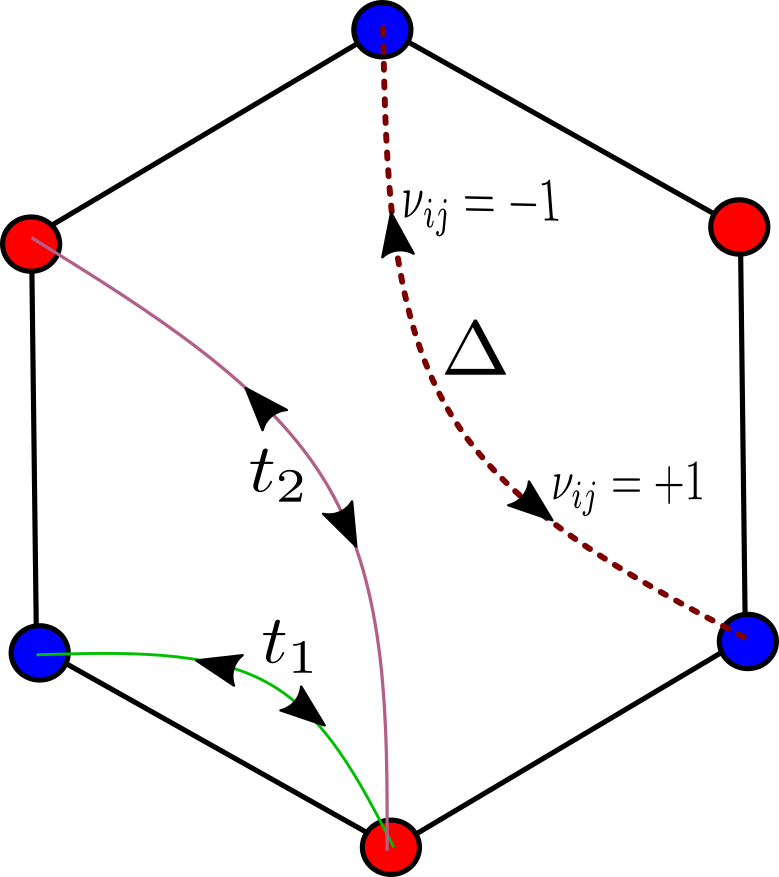
\includegraphics[width=0.5\columnwidth]{../Figures/kmh.png}
\caption{A honycomb cell with NN hopping $t_1$, NNN hopping $t_2$ and intrinsic SOI $\Delta$. $\nu_{ij} = \pm 1$ depending on whether the electron traversing from $i$ to $j$ makes a right ($+1$) or a left turn ($-1$).}
\label{fig:MKMH}
\vspace*{-6pt}
\end{figure}

This corresponds to the case $\bs{\Delta}_{1,ij} = 0$ and $\bs{\Delta}_{2,ij} = (0, 0, i \nu_{ij} \Delta)$ in \ref{BigHam}. The Hamiltonian parameters are sketched in Figure \ref{fig:MKMH}. With this, the effective Hamiltonian will be:

\begin{equation}
\label{MKMHeff}
\hat{H}_{\text{eff}}(t) = \sum_{\langle i,j \rangle} J_{1,ij}\bs{S}_i\bs{S}_j + \sum_{\langle \langle i,j \rangle \rangle} \left\{ J_{2,ij}\bs{S}_i\bs{S}_j + \bs{D}_{2,ij} \bs{S}_i \times \bs{S}_j + \bs{S}_i \bs{\Gamma}_{ij} \bs{S}_j \right\}
\end{equation}

Where:

\begin{align*}
J_{1,ij} &= t_1^2\mathcal{M}(\alpha_{ij}, \text{U}, \omega, t) \\
J_{2,ij} &= t_2^2\mathcal{M}(\alpha_{ij}, \text{U}, \omega, t) \\
\bs{D}_{2,ij} &= - 2\nu_{ij} t_2 \Delta \hat{e}_z \mathcal{M}(\alpha_{ij}, \text{U}, \omega, t) \\
\bs{\Gamma}_{2,ij} &= \Delta^2 \text{diag}(-1,-1,1) \mathcal{M}(\alpha_{ij}, \text{U}, \omega, t) 
\end{align*}

Such a Hamiltonian was first proposed by S. A. Owerre to model honeycome topological magnon insulators \cite{Owerre2016} \cite{Elyasi2018}. Experimental results regarding topological properties of spin waves in honeycomb ferromagnet Cr$I_3$ can only be understood by considering this Hamiltonian \cite{Chen2018}. This model is also relevant for the study of Spin Hall effects of Weyl magnons \cite{Zyuzin2018} \cite{Sekine2016}.

Now, a Hamiltonian with the form $\hat{H} = \sum_{\langle i,j \rangle} J_1 \bs{S}_i\bs{S}_j + \sum_{\langle \langle i,j \rangle \rangle} J_2\bs{S}_i\bs{S}_j$ is known as the $J_1$-$J_2$ Heisenberg model and in a 2D honeycomb lattice it exhibits N\'eel order for $J_2 < J_1 / 6$ and for $J_2 > J_1 / 6$ spin density waves (SDW) appear \cite{Mulder2010}. In the presence of DMI alone there will always be SDW in the plane perpendicular to $\bs{D}$ \cite{Uchida2006}. In Hamiltonian \ref{MKMHeff} we expect SDW to appear in the ground state and the SDW wavevector will be determined by a function of the parameters of this model. In the next section we will do a numerical of study on how modifying the ratio between NN and NNN spin interaction factors can change the spin state of the system.

\end{subsection}

\begin{subsection}{Time independent electric field in the NN + NNN Hamiltonian}

Now, let us examine the case in which the applied electric field is time independent. In this case the effective Hamiltonian is \ref{TimeIndepHeff}, which is the same Hamiltonian obtained when no electric field is applied except for a shift in the intermediate energy by $\pm \omega_0 = e\bs{\vec{R}}_{ij}\bs{\vec{E}}_0$. In this case, if we consider a Hamiltonian such as \ref{BigHam}, we can follow the same procedure done before: we plug in the hopping amplitudes \ref{BigHamHoppingAmp} into \ref{TimeIndepHeff} and apply \ref{SpinRel1} to sum over the spin states and obtain the corresponding spin Hamiltonian. We obtain:

\begin{align}
\hat{H}_{\text{eff}}(t) = &\sum_{\langle i,j \rangle ^*} \left\{ J_{1,ij}\bs{S}_i\bs{S}_j + \bs{D}_{1,ij} \bs{S}_i \times \bs{S}_j + \bs{S}_i\bs{\Gamma}_{1,ij}\bs{S}_j\right\} + \nonumber \\
&\sum_{\langle \langle i,j \rangle \rangle^*} \left\{ J_{2,ij}\bs{S}_i\bs{S}_j + \bs{D}_{2,ij} \bs{S}_i \times \bs{S}_j + \bs{S}_i\bs{\Gamma}_{2,ij}\bs{S}_j\right\}
\end{align}

$\langle i,j \rangle ^*$ denotes sum over NN avoiding repeating the same two sites. The coupling factors are:

\begin{align}
J_{n,ij} &= 4\frac{t_n^2}{U^*_{ij}} \\
\bs{D}_{n,ij} &= 8\frac{t_n i\bs{\Delta}_{n,ij}}{U^*_{ij}} \\
\Gamma_{n,ij}^{\alpha \beta} &= \frac{4}{U^*_{ij}}(\delta_{\alpha \beta} \bs{\Delta}_{n,ij}^2 - 2\Delta_{n,ij}^\alpha\Delta_{n,ij}^\beta )
\end{align}

Where:

\begin{equation}
\frac{1}{U^*_{ij}} =  \frac{1}{2}\left( \frac{1}{\text{U} - e\bs{\vec{R}}_{ij}\bs{\vec{E}}_0} + \frac{1}{\text{U} + e\bs{\vec{R}}_{ij}\bs{\vec{E}}_0} \right)
\end{equation}

\end{subsection}

\end{section}

\begin{section}{Numeric results}
\label{Numerics}

\begin{subsection}{One dimensional system}

We will start with a one dimensional chain with hamiltonian $\hat{H} = \sum_{\langle i,j \rangle} |J_1| \bs{S}_i\bs{S}_j + \sum_{\langle \langle i,j \rangle \rangle} \nu_{ij}|D_2|\hat{e}_z\bs{S}_i \times \bs{S}_j$. This approximated Hamiltonian with no NNN exchange interaction is very simple, but it can describe some systems where it has even been observed $|\bs{D}_{2,ij}| > |J_{2,ij}|$ \cite{Chen2018}. In this case we can write $\bs{S}(r) = S(\cos(kr), \sin(kr), 0)$, where the real number $k$ plays the role of the wavevector, and $\theta = ka-\pi$ is the deviation from the N\'eel state. Then the classical energy per site is given by:

\begin{equation}
\frac{E(\theta)}{2S^2} = -|J_1|\cos(\theta) + |D_2|\sin(2 \theta)
\end{equation}

and the energy is minimized for $\theta^* = \arcsin(\frac{\frac{J1}{D2} - \sqrt{(\frac{J1}{D2})^2+32}}{8})$, i.e. $\theta^* = \theta^*(\frac{J1}{D2})$. Next we will show numerically that the ratio between the NN and NNN parameters, $\frac{J1}{D2}$, can be modulated by the intensity of the field, and therefore the field can be used to control the SDW wavevector. 

We will use the time average approximation \ref{MFactorApprox0} so that we can write:

\begin{align}
J_{1,ij} &= J_{1,ij}^0  \sum_{n} \frac{\mathcal{J}_n(\alpha_{ij})^2}{1+n\frac{\omega}{\text{U}}} \\
D_{2,ij} &= D_{2,ij}^0  \sum_{n} \frac{\mathcal{J}_n(\alpha_{ij})^2}{1+n\frac{\omega}{\text{U}}}
\end{align}

Where $\bs{D}_{2,ij} = \hat{e}_z D_{2,ij}$ and where $J_{1,ij}^0 = J_{1}^0 = \frac{2t_1^2}{\text{U}}$ and $D_{2,ij}^0 = -\frac{4t_2\Delta\nu_{ij}}{\text{U}}$. Since $\mathcal{J}_n(-x) = (-1)^n\mathcal{J}_n(x)$ the dependance is on $|\alpha_{ij}|$ only. Now, using \ref{Def_alpha}, for circularly polarized light we have $|\alpha_{ij}| = \frac{1}{\sqrt{2}}e|\vec{R}_{ij}| \frac{E_0}{\omega} = \frac{1}{\sqrt{2}}ea \frac{E_0}{\omega} \frac{|\vec{R}_{ij}|}{a} = \frac{|\vec{R}_{ij}|}{\sqrt{2}a} \mathcal{E}$, where $a$ is the lattice constant and $\mathcal{E} = \frac{eaE_0}{\omega}$. Now, for $J_{1,ij}$, $i$ and $j$ are NN and so we can write $|\vec{R}_{ij}|=a$, whereas for $D_{2,ij}$, $i$ and $j$ are NNN and so $|\vec{R}_{ij}|=2a$. Thus:

\begin{align}
J_{1,ij} &= J_{1} = J_{1}^0  \sum_{n} \frac{\mathcal{J}_n(\frac{1}{\sqrt{2}}\mathcal{E})^2}{1+n\frac{\omega}{\text{U}}} \\
D_{2,ij} &= D_{2,ij}^0  \sum_{n} \frac{\mathcal{J}_n(\sqrt{2}\mathcal{E})^2}{1+n\frac{\omega}{\text{U}}}
\end{align}

In each case the absolute vale is independent of $i,j$.  Now, in units $\hbar=t_1=1$ we measure energy in units of $t_1$ and frequency in units of $\frac{t_1}{\hbar}$. Then, for $t_2 = 0.1$, $\Delta = 0.5$, $\text{U} = 10$ and $\omega = 6, 16$ we obtain \ref{Fig1:NNvsNNN}. The ratio $\frac{J_{1,ij}}{D_{2,ij}}$ is plotted in \ref{Fig1:ratio}. Finally, in \ref{Fig2} we plot the SDW NN angle $\theta$.

\begin{figure}
\centering
\begin{subfigure}{.45\textwidth}
  %\centering
  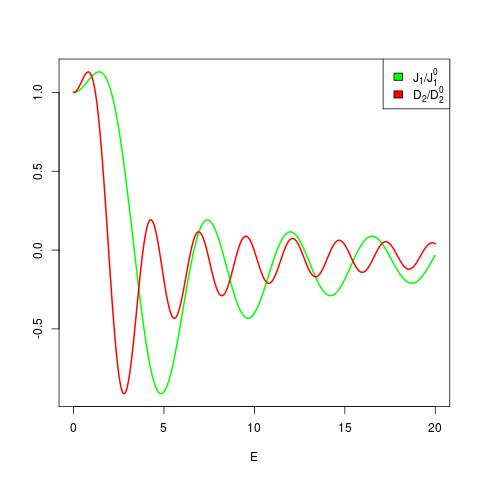
\includegraphics[width=1\linewidth]{Chapters/NNvsNNN.pdf}
  \caption{$\frac{J_{1}}{J_{1}^0}$ and $\frac{D_{2,ij}}{D_{2,ij}^0}$ are plotted as function of $\mathcal{E}$. Similar results are obtained in \cite{Mentink2015} for $J_{1}$. Solid lines are for $\omega = 6$ and dashed lines are for $\omega = 16$.}
  \label{Fig1:NNvsNNN}
\end{subfigure}%
\hspace*{\fill}
\begin{subfigure}{.45\textwidth}
  %\centering
  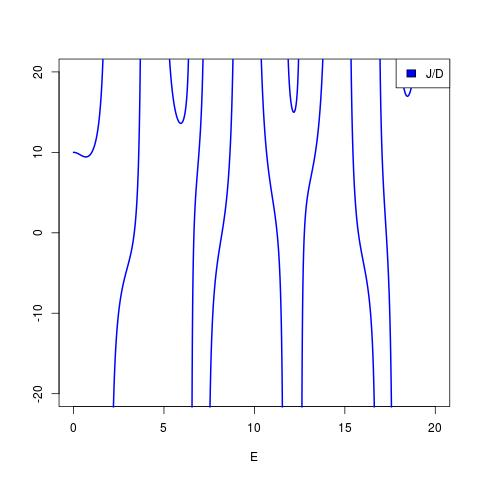
\includegraphics[width=1\linewidth]{Chapters/ratio.pdf}
  \caption{$\frac{J_{1}}{D_{2,ij}}$ is plotted as function of $\mathcal{E}$, it diverges every time $D_{2,ij}$ changes sign. Solid lines are for $\omega = 6$ and dashed lines are for $\omega = 16$.}
  \label{Fig1:ratio}
\end{subfigure}
\label{Fig1}
\end{figure}

\begin{figure}
\centering
  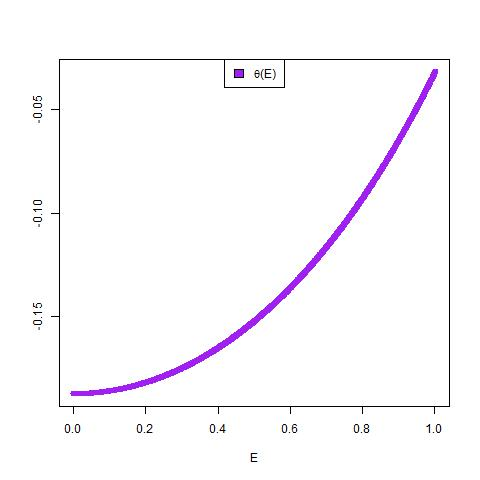
\includegraphics[width=0.5\linewidth]{Chapters/theta.pdf}
  \caption{The spin wave density NN angle $\theta$ as a function of $\mathcal{E}$. The field modifies the ratio $\frac{J_{1}}{D_{2,ij}}$ thus modifying the wave vector. Solid lines are for $\omega = 6$ and dashed lines are for $\omega = 16$.}
\label{Fig2}
\end{figure}

\end{subsection}

\begin{subsection}{Two dimensional systems}
 
In a honeycomb lattice described by \ref{MKMHeff} the usual approach is to write:



\end{subsection}

\end{section}


%\chapter{Perturbing the lattice}
\label{ChapPerturbing}

In this chapter we will derive an effective spin Hamiltonian for different models in the presence of a high frequency electromagnetic perturbation. The goal is to manipulate $J$ and $\bs{D}_{ij}$ in \ref{HeffNOEMF} separately. This has already been done for the case of Mott insulators (\cite{Mentink2015}, \cite{Kitamura2017}) where the starting Hamiltonian is the Hubbard model:

\begin{equation*}
\hat{H} = -t_0\sum_{\langle i,j \rangle, \sigma} \hat{c}_{i \sigma}^\dagger \hat{c}_{j \sigma} + \text{U} \sum_{i=1}^M \hat{n}_{i\uparrow}\hat{n}_{i\downarrow}
\end{equation*} 

In this model, since SOI is not taken into account, only the exchange interaction $J$ plays a role. The electromagnetic perturbation is then introduced via the Peierls substitution. We reproduce the result in section \ref{Section3Hubbard}. In the following sections we extend the analysis to different systems with spin orbit interaction thereby modulating $\bs{D}_{ij}$ or other spin interactions. The simplest model with spin orbit interaction is \ref{Hubbard}:

\begin{equation*}
\hat{H} = -\sum_{\langle i,j \rangle, \sigma, \sigma'}(\delta_{\sigma, \sigma'} t_{0} + \bs{\Delta}_{ij} \bs{\sigma}_{\sigma, \sigma'})\hat{c}_{i \sigma}^\dagger \hat{c}_{j \sigma'} + \text{U} \sum_{i=1}^M \hat{n}_{i\uparrow}\hat{n}_{i\downarrow}
\end{equation*}

Which is the same Hubbard model plus a spin dependent hopping term, which represents Rashba SOI for $\bs{\Delta}_{ij} = i\Delta_R(R_{ij}^y, -R_{ij}^x, 0)$ or Dresselhaus SOI for $\bs{\Delta}_{ij} = i\Delta_R(R_{ij}^x, -R_{ij}^y, 0)$. In section \ref{Section3HubbardSOI} we show how the exchange interaction and the DMI couplings are modulated in presence of an electromagnetic field.  

In the case of graphene or other coplanar honeycomb lattice structures, nearest neighbor Rashba terms are not allowed by symmetry, and only next nearest neighbor (NNN) spin conserving terms contribute \cite{Kane2005}, this term opens a gap in the band structure describing a topological insulator. For this case we examine the Kane-Mele-Hubbard model. The effective spin model of this Hamiltonian contains the usual exchange interaction and DMI and, in addition, it exhibits anisotropic exchange interaction arising from the intrinsic SOI term. This new term has already been obtained in \cite{Rachel2010} without taking into account any electromagnetic field.

Non-coplanar honeycomb lattice may exhibit intrinsic Rashba interactions between NNN \cite{Liu2011}, this, together with a NNN hopping (which would arise from direct overlapping of the next nearest neighbor Wannier functions or from second order processes) will lead to NNN DMI.


\begin{section}{Time dependent effective Hamiltonian}
\label{SectionTDHeff}

In this section we will derive a general effective Hamiltonian starting with any Hamiltonian that can be written as:

\begin{equation}
\hat{H} = -\hat{T} + \text{U}\hat{D}
\end{equation}
Where $\hat{D} = \sum_{i=1}^M \hat{n}_{i\uparrow}\hat{n}_{i\downarrow}$ is the doublon number operator and $\hat{T}$ is any hopping operator. In terms of on-site creation and annihilation operators we can write the hopping operator as $\hat{T} = \sum_{i,j, \sigma, \sigma'} t_{ij}^{\sigma \sigma'} \hat{c}_{i \sigma}^\dagger \hat{c}_{j \sigma'}$. The strength of the on-site interaction $\text{U}$ is much larger than the hopping amplitude, therefore, in a half filling system the zero double occupancies subspace $d=0$ can be taken as the low energy subspace in which the effective Hamiltonian will act.

The effect of the electromagnetic perturbation in the lattice can be introduced via the Peierls substitution (\ref{AP3A}). With this notation, in presence of a vector potential $\vec{A}(t)$ (which we assume to not vary noticeably in the scale of the lattice) the Peierls substitution leads to an extra time dependent phase in the hopping amplitude:

\begin{equation}
\label{TimeDepHopping}
t_{ij}^{\sigma \sigma'}(t) = t_{ij}^{\sigma \sigma'} e^{ie\bs{R}_{ij}\cdot\bs{A}(t)}
\end{equation}
Where $\bs{A}$ is the vector potential and $\bs{R}_{ij} = \bs{R}_i-\bs{R}_j$ and we take $\hbar=1$. We write the electric field as $\bs{E}(t) = \frac{1}{2}(\vec{E}e^{-i\omega t}+\vec{E}^*e^{i\omega t})$, where $\vec{E} = E_0\hat{e}$ and $\hat{e} = \frac{1}{\sqrt{1+\lambda_{POL}^2}}(\hat{e}_x+i\lambda_{POL}\hat{e}_y)$ is the polarization vector and $\lambda_{POL} = 0, \pm 1$ for plane polarized, right handed and left handed circular polarized field respectively. The vector potential takes the form $\bs{A}(t) = \frac{1}{2}(\vec{A}e^{-i\omega t} + \vec{A}^* e^{i\omega t})$, with $\vec{A} = \frac{iE_0}{\omega}\hat{e}$.
With the hopping amplitudes in \ref{TimeDepHopping} the Hamiltonian becomes time dependent. We will use Floquet theory \ref{APE} to derive an effective Hamiltonian including the laser perturbation.

Let us define:

\begin{equation}
\label{Def_alpha}
e\bs{R}_{ij}\vec{A} = \alpha_{ij} e^{i \theta_{ij}}
\end{equation}
With $\alpha_{ij} = \pm|e\bs{R}_{ij}\vec{A}|$ in such a way that:

\begin{align}
\alpha_{ij} &= -\alpha_{ji} \label{alphaSym} \\
\theta_{ij} &= \theta_{ji} \label{thetaSym}
\end{align}
and $\theta_{ij} \in \left[0,\pi\right)$. Then we can apply the Jacobi–Anger expansion:

\begin{align*}
t_{ij}^{\sigma \sigma'}(t) &= t_{ij}^{\sigma \sigma'}e^{ie\bs{R}_{ij}\cdot\bs{A}(t)} = t_{ij}^{\sigma \sigma'}e^{i\alpha_{ij} \cos(\omega t - \theta_{ij})} = \\
&= t_{ij}^{\sigma \sigma'}\sum_m e^{i(\frac{\pi}{2}-\theta_{ij})m} \mathcal{J}_m(\alpha_{ij}) e^{im\omega t} = \sum t_{ij,m}^{\sigma \sigma'} e^{im\omega t}
\end{align*}
Where we defined 

\begin{equation}
\label{HoppAmpFourier}
t_{ij,m}^{\sigma \sigma'} = t_{ij}^{\sigma \sigma'} e^{i(\frac{\pi}{2}-\theta_{ij})m} \mathcal{J}_m(\alpha_{ij})
\end{equation}
Which is the \textit{m}th Fourier mode of the hopping term and $\mathcal{J}_m(x)$ is the \textit{m}th Bessel function \cite{Kitamura2017}. Correspondingly we can write $\hat{T}(t) = \sum_m \hat{T}_m e^{im \omega t}$ where $\hat{T}_m$ is the sum of all the \textit{m}th Fourier mode of the hopping terms. We can further decompose the hopping operator into:

\begin{equation}
\hat{T}(t) = \sum_m (\hat{T}_{-1,m}+\hat{T}_{0,m}+\hat{T}_{1,m})e^{im\omega t}
\end{equation}
Where $\hat{T}_{dm}(t)$ changes the doublon number by $d$, for example, if $\hat{P}_d$ is the projection operator into the subspace with doublon number $d$, then $\hat{T}_{dm}(t) = \sum_i \hat{P}_{i+d}\hat{T}_{m}(t)\hat{P}_i$. Since the hopping term is of second order in the creation and annihilation operators, it can change the double occupancy of the states only by $\pm1$.

In order to derive the form of the effective spin Hamiltonian let us introduce a time dependent unitary transformation $\hat{U}(t) = e^{-i\hat{S}(t)}$. The transformed Hamiltonian is:

\begin{equation}
\hat{H}'(t) = e^{i\hat{S}(t)} \hat{H}(t) e^{-i\hat{S}(t)} - e^{i\hat{S}(t)} id_t e^{-i\hat{S}(t)}
\end{equation} 
We perform the unitary transformation perturbatively in the hopping operator, we can formally write $\hat{T}(t) = \eta \hat{T}(t)$, where $\eta$ will play the role of a bookkeeping parameter in the perturbative expansion. We expand $\hat{S}(t) = \sum_\nu \eta^\nu \hat{S}^{(\nu)}(t)$ and $\hat{H}'(t) = \sum_\nu \eta^\nu \hat{H}'^{(\nu)}(t)$. We require the transformed Hamiltonian to be block diagonal in the doublon number operator $\hat{d}$. To fulfill this requirement, the unitary transformation $\hat{S}(t)$ must have the same periodicity as $\hat{T}(t)$; consequently, the transformed Hamiltonian $\hat{H}'(t)$ will have the same periodicity as the original Hamiltonian $\hat{H}(t)$. Thus we can write $\hat{S}^{(\nu)}(t) = \sum_m e^{im\omega t}\hat{S}^{(\nu)}_m$. With the further requirement that $\hat{S}(t)$ does not contain block-diagonal terms, we can uniquely determine the unitary transformation:

\begin{equation}
\hat{S}^{(\nu)}(t) = \sum_{d \neq 0} \sum_m \eta^\nu \hat{S}^{(\nu)}_{d,m} e^{im\omega t}
\end{equation}
where $\hat{S}^{(\nu)}_{d,m}$ changes the double occupancy number by $d$.

Now we can use the identity:

\begin{equation}
id_t e^{-i\hat{S}(t)} = \sum_n \frac{1}{(n+1)!}\text{ad}_{-i\hat{S}(t)}^n (d_t \hat{S}(t))e^{-i\hat{S}(t)}
\end{equation}
Derived in appendix \ref{AP3B}, where $\text{ad}_A(B) = [A,B]$ to rewrite the transformed Hamiltonian as:

\begin{equation}
\hat{H}'(t) = e^{i\hat{S}(t)} \left( \hat{H}(t) - \sum_n \frac{1}{(n+1)!}\text{ad}_{-i\hat{S}(t)}^n (d_t \hat{S}(t)) \right) e^{-i\hat{S}(t)}
\end{equation}
Using the Baker–Campbell–Hausdorff expansion we can write the transformed Hamiltonian as:

\begin{equation}
\label{PertFull}
\hat{H}'(t) = \sum_m \frac{1}{m!} \text{ad}_{i\hat{S}(t)}^m \left( \hat{H}(t) - \sum_n \frac{1}{(n+1)!}\text{ad}_{-i\hat{S}(t)}^n (d_t \hat{S}(t)) \right)
\end{equation}
Now, in this expression we have to expand $\hat{S}(t) = \sum_\nu \eta^\nu \hat{S}^{(\nu)}(t)$ and $\hat{H}'(t) = \sum_\nu \eta^\nu \hat{H}'^{(\nu)}(t)$ and determine $\hat{S}^{(\nu)}(t)$ iteratively in $\nu$ so that $\hat{H}'^{(\nu)}(t)$ is diagonal in the doublon number. Notice that we do not expand $\hat{H}(t)$ as an infinite series since $\hat{H}(t) = -\eta \hat{T}(t) + \text{U}\hat{D}$. Now, notice also that if we take $i\hat{S}^{(0)}(t)=0$ in \ref{PertFull}, then, to zeroth order in $\eta$ only terms in $m=0$ and $n=0$ contribute obtaining:

\begin{equation}
\hat{H}'^{(0)}(t) = \text{U}\hat{D}
\end{equation}
Which is indeed diagonal in the doublon number, and therefore we can take $i\hat{S}^{(0)}(t)=0$. With this equating terms of the same order in \ref{PertFull} is greatly simplified, since terms with high $m,n$ will correspond to terms with high $\eta$. Since we are only interested in orders up to second order, we can truncate \ref{PertFull} up to $m=2$:

\begin{align}
\label{PertTrunc}
\hat{H}'(t) &=  \hat{H}(t) - \sum_n \frac{1}{(n+1)!}\text{ad}_{-i\hat{S}(t)}^n (d_t \hat{S}(t)) + [i\hat{S}(t), \hat{H}(t) - \sum_n \frac{1}{(n+1)!}\text{ad}_{-i\hat{S}(t)}^n (d_t \hat{S}(t))] + \nonumber \\
&+ \frac{1}{2} [i\hat{S}(t),[i\hat{S}(t), \hat{H}(t) - \sum_n \frac{1}{(n+1)!}\text{ad}_{-i\hat{S}(t)}^n (d_t \hat{S}(t)) ]]
\end{align}
This equation holds up to order $\eta^2$. In first order we obtain:

\begin{equation}
\label{1stO}
\hat{H}'^{(1)}(t) = -\hat{T}(t) - d_t\hat{S}^{(1)}(t) + \left[ i\hat{S}^{(1)}(t), \text{U}\hat{D} \right]
\end{equation}
Now we expanding in $m,d$ and use $\left[ \hat{D}, \hat{S}^{(\nu)}_{dm} \right] = d\hat{S}^{(\nu)}_{dm}$ because $\hat{S}^{(\nu)}_{dm}$ changes the doublon number by $d$:

\begin{equation}
\hat{H}'^{(1)}(t)=-\hat{T}(t)-\sum_{d\neq 0}\sum_m (\text{U}d+m\omega) i\hat{S}^{(1)}_{dm} e^{im\omega t}
\end{equation}
Therefore:

\begin{align}
i\hat{S}^{(1)}_d(t) &= -\sum_m \frac{\hat{T}_{d,m}}{\text{U}d+m\omega}e^{im\omega t} \label{1stOSpin}\\
\hat{H}'^{(1)}(t) &= -\sum_m \hat{T}_{0,m}(t)e^{im\omega t} \label{1stOH}
\end{align}
To second order we find:

\begin{align}
\hat{H}'^{(2)}(t) &= - d_t\hat{S}^{(2)}(t) - \frac{1}{2}\left[-i\hat{S}^{(1)}(t), d_t\hat{S}^{(1)}(t) \right] + \left[i\hat{S}^{(1)}(t), -\hat{T}(t)-\frac{1}{2}d_t\hat{S}^{(1)}(t) \right] +\nonumber \\
&+ \left[i\hat{S}^{(2)}(t), \text{U}\hat{D} \right] + \frac{1}{2} \left[i\hat{S}^{(1)}(t), \left[i\hat{S}^{(1)}(t), \text{U}\hat{D} \right] \right] = \nonumber \\
&= \left[i\hat{S}^{(2)}(t), \text{U} \hat{D} \right] - \left[ i\hat{S}^{(1)}(t), \hat{T}(t) \right] + \frac{1}{2}\left[ i\hat{S}^{(1)}(t), \left[ i\hat{S}^{(1)}(t), \text{U}\hat{D} \right] \right] - d_t\hat{S}^{(2)}(t)
\end{align}
Using \ref{1stO} and using $\left[ i\hat{S}^{(1)}(t), d_t\hat{S}^{(1)}(t)\right] = 0$ due to different Fourier modes of the hopping operator being equal up to a constant (explain better), we can rewrite:

\begin{equation}
\hat{H}'^{(2)}(t) = \left[i\hat{S}^{(2)}(t), \text{U} \hat{D} \right] - \frac{1}{2}\left[ i\hat{S}^{(1)}(t), \hat{T}(t) - \hat{H}'^{(1)}(t)\right] - d_t\hat{S}^{(2)}(t)
\end{equation}
Using \ref{1stOSpin} and \ref{1stOH}, the middle term is:

\begin{align*}
&\left[ i\hat{S}^{(1)}(t), \hat{T}(t) - \hat{H}'^{(1)}(t)\right] = -\left[\sum_m \left( \frac{\hat{T}_{1m}}{\text{U}+m\omega} - \frac{\hat{T}_{-1m}}{\text{U}-m\omega} \right)e^{im \omega t}, \sum_n \left( \hat{T}_{-1n} + 2\hat{T}_{0n} + \hat{T}_{1n} \right) e^{in\omega t} \right] \\
&= -\sum_{mn} \left\{ \frac{2\left[\hat{T}_{1m}, \hat{T}_{0n} \right]}{\text{U}+m\omega} + \frac{\left[\hat{T}_{1m}, \hat{T}_{-1n} \right]}{\text{U}+m\omega} - \frac{\left[\hat{T}_{-1m}, \hat{T}_{1n} \right]}{\text{U}-m\omega} - \frac{2\left[\hat{T}_{-1m}, \hat{T}_{0n} \right]}{\text{U}-m\omega} \right\} e^{i(m+n)\omega t} \\
&= -\sum_{mn} \left\{ \frac{2\left[\hat{T}_{1n}, \hat{T}_{0(m-n)} \right]}{\text{U}+n\omega} + \frac{\left[\hat{T}_{1n}, \hat{T}_{-1(m-n)} \right]}{\text{U}+n\omega} - \frac{\left[\hat{T}_{-1n}, \hat{T}_{1(m-n)} \right]}{\text{U}-n\omega} - \frac{2\left[\hat{T}_{-1n}, \hat{T}_{0(m-n)} \right]}{\text{U}-n\omega} \right\} e^{im\omega t}
\end{align*}
Altogether:

\begin{align*}
\hat{H}'^{(2)}(t) &= \sum_{mn} \left\{ \frac{\left[\hat{T}_{1n}, \hat{T}_{0(m-n)} \right]}{\text{U}+n\omega} + \frac{\left[\hat{T}_{1n}, \hat{T}_{-1(m-n)} \right]}{2(\text{U}+n\omega)} - \frac{\left[\hat{T}_{-1n}, \hat{T}_{1(m-n)} \right]}{2(\text{U}-n\omega)} - \frac{\left[\hat{T}_{-1n}, \hat{T}_{0(m-n)} \right]}{\text{U}-n\omega} \right\} e^{im\omega t} \\
&-\sum_{d\neq 0}\sum_m (\text{U}d+m\omega) i\hat{S}^{(2)}_{dm} e^{im\omega t}
\end{align*}
By choosing $i\hat{S}^{(2)}_{dm}$ such that the transformed Hamiltonian is block-diagonal, we obtain:

\begin{align}
i\hat{S}^{(2)}_{dm} &= \sum_n \frac{\left[ \hat{T}_{dn}, \hat{T}_{0(m-n)} \right]}{(\text{U}d+n\omega)(\text{U}d+m\omega)} \label{2ndOSpin}\\
\hat{H}'^{(2)}(t) &= \frac{1}{2}\sum_{mn} \left( \frac{\left[\hat{T}_{1n}, \hat{T}_{-1(m-n)} \right]}{\text{U}+n\omega} - \frac{\left[\hat{T}_{-1n}, \hat{T}_{1(m-n)} \right]}{\text{U}-n\omega} \right) e^{im\omega t} \label{2ndOH}
\end{align}
Now the effective Hamiltonian acts on the subspace of $d=0$ (zero double occupancies), therefore we are only interested on the block $\hat{P}_0 \hat{H}'^{(2)}(t) \hat{P}_0$ (notice that $\hat{P}_0 \hat{H}'^{(1)}(t) \hat{P}_0 = 0$). In this subspace we can write:

\begin{align}
\hat{H}_{\text{eff}}(t) &= \hat{P}_0\hat{H}'^{(2)}(t)\hat{P}_0 = -\frac{1}{2}\sum_{mn} \left( \frac{\hat{P}_0  \hat{T}_{-1(m-n)}\hat{T}_{1n}\hat{P}_0}{\text{U}+n\omega} + \frac{\hat{P}_0 \hat{T}_{-1n} \hat{T}_{1(m-n)} \hat{P}_0}{\text{U}-n\omega} \right) e^{im\omega t} \nonumber \\
&= -\frac{1}{2}\sum_{mn} \left\{ \frac{\hat{P}_0  (\hat{T}_{-1(m-n)}\hat{T}_{1n} + \hat{T}_{-1-n}\hat{T}_{1(m+n)})\hat{P}_0}{\text{U}+n\omega} \right\} e^{im\omega t} \label{2ndOHeff}
\end{align}
Now, since the hopping operators act on the subspace $d=0$ and must remain within that subspace, therefore $\hat{P}_0 \hat{T}_{-1a} \hat{T}_{1b} \hat{P}_0$ will be a sum of all possible hoppings between two different sites:

\begin{align*}
\hat{P}_0 \hat{T}_{-1a} \hat{T}_{1b} \hat{P}_0 = \sum_{i,j, \sigma_1, \sigma_2, \sigma_3, \sigma_4} t_{ij,a}^{\sigma_1 \sigma_2} t_{ji,b}^{\sigma_3 \sigma_4} \hat{c}_{i \sigma_1}^\dagger \hat{c}_{j \sigma_2} \hat{c}_{j \sigma_3}^\dagger \hat{c}_{i \sigma_4}
\end{align*}
Where $a$ and $b$ are any two Fourier modes. Inserting this into \ref{HeffSimplified} and using the definition of $t_{ij,m}^{\sigma \sigma'} = t_{ij}^{\sigma \sigma'} e^{i(\frac{\pi}{2}-\theta_{ij})m} \mathcal{J}_m(\alpha_{ij})$ and using that $\theta_{ji} = \theta_{ij}$ and $\alpha_{ji} = -\alpha_{ij}$ and the properties $\mathcal{J}_{-m}(x) = (-1)^m\mathcal{J}_m(x)$ and $\mathcal{J}_m(-x) = (-1)^m\mathcal{J}_m(x)$ we can write \ref{HeffSimplified} as:

\begin{align}
&\hat{H}_{\text{eff}}(t) = \hat{P}_0\hat{H}'^{(2)}(t)\hat{P}_0 = - \frac{1}{2}\sum_{mn} \sum_{i,j, \sigma_1, \sigma_2, \sigma_3, \sigma_4}\hat{c}_{i \sigma_1}^\dagger \hat{c}_{j \sigma_2} \hat{c}_{j \sigma_3}^\dagger \hat{c}_{i \sigma_4} \frac{t_{ij,m-n}^{\sigma_1 \sigma_2} t_{ji,n}^{\sigma_3 \sigma_4} + t_{ij,-n}^{\sigma_1 \sigma_2} t_{ji,m+n}^{\sigma_3 \sigma_4}}{\text{U}+n\omega} e^{im\omega t} \nonumber \\
&= - \frac{1}{2}\sum_{mn} \sum_{i,j, \sigma_1, \sigma_2, \sigma_3, \sigma_4} \left\{ \hat{c}_{i \sigma_1}^\dagger \hat{c}_{j \sigma_2} \hat{c}_{j \sigma_3}^\dagger \hat{c}_{i \sigma_4} t_{ij}^{\sigma_1 \sigma_2} t_{ji}^{\sigma_3 \sigma_4} e^{i(\frac{\pi}{2}-\theta_{ij})m} \right. \nonumber \\
& \left. \frac{ \mathcal{J}_{m-n}(\alpha_{ij}) \mathcal{J}_{n}(\alpha_{ji}) + \mathcal{J}_{-n}(\alpha_{ij}) \mathcal{J}_{m+n}(\alpha_{ji})}{\text{U}+n\omega} e^{im\omega t} \right\} \nonumber \\
&= - \frac{1}{2}\sum_{mn} \sum_{i,j, \sigma_1, \sigma_2, \sigma_3, \sigma_4} \left\{ \hat{c}_{i \sigma_1}^\dagger \hat{c}_{j \sigma_2} \hat{c}_{j \sigma_3}^\dagger \hat{c}_{i \sigma_4} t_{ij}^{\sigma_1 \sigma_2} t_{ji}^{\sigma_3 \sigma_4} e^{i(\frac{\pi}{2}-\theta_{ij})m} (-1)^m \right. \nonumber \\
&\left. \frac{ \mathcal{J}_{n-m}(\alpha_{ij}) \mathcal{J}_{n}(\alpha_{ij}) + \mathcal{J}_{n}(\alpha_{ij}) \mathcal{J}_{m+n}(\alpha_{ij})}{\text{U}+n\omega} e^{im\omega t} \right\} \nonumber \\
&= - \frac{1}{2} \sum_{i,j, \sigma_1, \sigma_2, \sigma_3, \sigma_4}\hat{c}_{i \sigma_1}^\dagger \hat{c}_{j \sigma_2} \hat{c}_{j \sigma_3}^\dagger \hat{c}_{i \sigma_4} t_{ij}^{\sigma_1 \sigma_2} t_{ji}^{\sigma_3 \sigma_4} \mathcal{M}(\alpha_{ij}, \text{U}, \omega, t) \label{HeffSimplified}
\end{align}
Where we defined:

\begin{equation}
\mathcal{M}(\alpha_{ij}, \text{U}, \omega, t) = \sum_{mn}e^{-i(\frac{\pi}{2}+\theta_{ij})m} \left\{ 
    \frac{\mathcal{J}_{n-m}(\alpha_{ij})\mathcal{J}_{n}(\alpha_{ij}) + \mathcal{J}_{n}(\alpha_{ij})\mathcal{J}_{m+n}(\alpha_{ij})}{\text{U}+n\omega} \right\}e^{im\omega t}
\end{equation}
In the following sections we will use this effective Hamiltonian for different models of the hopping operator. In each case we will introduce the spin relations \ref{SpinOperatorInv1} and \ref{SpinOperatorInv2} together with \ref{SpinRel1}, \ref{SpinRel2} and \ref{SpinRel3} to obtain the corresponding effective spin Hamiltonian. 

\begin{subsection}{Time independent field}

Before we start using \ref{HeffSimplified} for different models we would like to investigate the case in which the electric field is time independent. In that case we can restrict the analysis to the one dimensional lattice, since in second order the electric field will only affect the bonds parallel to the field. Let us denote $\vec{\bs{E}} = E_0 \hat{e}_x$, then the Peiels transformed hopping amplitudes can be written as:

\begin{equation}
\label{TimeIndepHoppingAmpl}
t_{ij}^{\sigma \sigma'} (t) = t_{ij}^{\sigma \sigma'} e^{ie \vec{\bs{R}}_{ij} \cdot \vec{\bs{E}} t}
\end{equation}
Therefore, there will be only two Fourier modes with frequency $\omega_0 = e \vec{\bs{R}}_{ij} \cdot \vec{\bs{E}} = \pm eaE_0$, where the sign $+(-)$ corresponds to the case $\vec{\bs{R}}_{ij} = \pm a \hat{e}_x$. Notice that this frequency $\omega_0$ does not correspond to a field frequency ($\vec{\bs{E}}$ is time independent), but to the Fourier mode in the hopping amplitudes (which is induced by the time independent field). From this point we can apply the same procedure as in the general case up to \ref{2ndOHeff}. We can greatly simplify this by considering that:
\begin{itemize}
	\item $n$ can only take values $ n = \pm 1$ (there are no additional Fourier modes).
	\item When restricted to the low energy subspace a product $\hat{T}_{-1 a} \hat{T}_{1 b}$ will only contribute when $a$ and $b$ have opposite signs ($a=1, b=-1$ or viceversa). This is because, in the low energy subspace $\hat{T}_{-1 a} \hat{T}_{1 b}$ can only represent a hopping from a site $i$ to a site $j$ and the hopping back to $i$, we can see from \ref{TimeIndepHoppingAmpl} that these two amplitudes will be in opposite Fourier modes.
\end{itemize}
Taking this into consideration we see that only $m=0$ terms will remain, which is consistent with the fact that the two phases cancel out in the process $i \rightarrow j \rightarrow i$. We can thus rewrite \ref{2ndOHeff} as:

\begin{equation}
\hat{H}_{\text{eff}} = -\hat{P}_0 \left\{ \frac{\hat{T}_{-1,1}\hat{T}_{1,-1} }{\text{U}-\omega_0} + \frac{\hat{T}_{-1,-1}\hat{T}_{1,1} }{\text{U}+\omega_0} \right\} \hat{P}_0
\end{equation}
Now, the first fraction represents a hopping process $i\rightarrow j \rightarrow i$ where $j$ lies left to $i$, whereas in the second fraction $j$ lies right to $i$:

\begin{align*}
\hat{P}_0 \hat{T}_{-1,1} \hat{T}_{1,-1} \hat{P}_0 &= \sum_{i > j, \sigma_1, \sigma_2, \sigma_3, \sigma_4} t_{ij}^{\sigma_1 \sigma_2} t_{ji}^{\sigma_3 \sigma_4} \hat{c}_{i \sigma_1}^\dagger \hat{c}_{j \sigma_2} \hat{c}_{j \sigma_3}^\dagger \hat{c}_{i \sigma_4} \\
\hat{P}_0 \hat{T}_{-1,-1} \hat{T}_{1,1} \hat{P}_0 &= \sum_{i < j, \sigma_1, \sigma_2, \sigma_3, \sigma_4} t_{ij}^{\sigma_1 \sigma_2} t_{ji}^{\sigma_3 \sigma_4} \hat{c}_{i \sigma_1}^\dagger \hat{c}_{j \sigma_2} \hat{c}_{j \sigma_3}^\dagger \hat{c}_{i \sigma_4} 
\end{align*}
We can rewrite this in the more compact form:

\begin{equation}
\label{TimeIndepHeff}
\hat{H}_{\text{eff}} = -\sum_{i, j, \sigma_1, \sigma_2, \sigma_3, \sigma_4} \frac{t_{ij}^{\sigma_1 \sigma_2} t_{ji}^{\sigma_3 \sigma_4} \hat{c}_{i \sigma_1}^\dagger \hat{c}_{j \sigma_2} \hat{c}_{j \sigma_3}^\dagger \hat{c}_{i \sigma_4}}{\text{U} + \text{sgn}(j-i)\omega_0}
\end{equation}
This is the same effective Hamiltonian obtained in the previous section without an electric field but with a shift in the intermediate state energy by $\pm \omega_0 = \pm eaE_0$. We will analyze the corresponding spin Hamiltonian of this effective Hamiltonian when we consider the Kane-Mele-Hubbard model in Section \ref{section3NNN}.

\end{subsection}

\end{section}


\begin{section}{Hubbard model without SOI}
\label{Section3Hubbard}
We start by considering the simplest hopping operator, excluding SOI terms \ref{HnoSOI}:

\begin{equation}
\hat{H} = -t_0\sum_{\langle i,j \rangle, \sigma} \hat{c}_{i \sigma}^\dagger \hat{c}_{j \sigma} + \text{U} \sum_{i=1}^M \hat{n}_{i\uparrow}\hat{n}_{i\downarrow}
\end{equation}

We see that the hopping amplitudes introduced in the previous section can be written as $t_{ij}^{\sigma \sigma'} = \delta_{\sigma \sigma'} t_0$ for $i,j$ being nearest neighbors, and $t_{ij}^{\sigma \sigma'} = 0$ otherwise. With this we can directly apply \ref{HeffSimplified} to obtain:

\begin{equation}
\hat{H}_{\text{eff}}(t) = -\frac{t_0^2}{2} \sum_{\langle i,j \rangle, \sigma, \sigma'} \hat{c}_{i \sigma}^\dagger \hat{c}_{j \sigma} \hat{c}_{j \sigma'}^\dagger \hat{c}_{i \sigma'} \mathcal{M}(\alpha_{ij}, \text{U}, \omega, t)
\end{equation}

Now, introducing the spin operators \ref{SpinOperatorInv1} and \ref{SpinOperatorInv2} and summing over the spin states as in \ref{SpinRel1}:

\begin{align*}
\sum_{\sigma, \sigma'} \hat{c}_{i \sigma}^\dagger \hat{c}_{j \sigma} \hat{c}_{j \sigma'}^\dagger \hat{c}_{i \sigma'} = \sum_{\sigma, \sigma'} \left( \frac{\delta_{\sigma \sigma'}}{2} + \bs{S}_i\cdot\bs{\sigma}_{\sigma' \sigma} \right) \left( \frac{\delta_{\sigma \sigma'}}{2} - \bs{S}_j\cdot\bs{\sigma}_{\sigma \sigma'} \right) = -2\bs{S}_i\cdot \bs{S}_j
\end{align*}

Where we neglected the constant term. The effective spin Hamiltonian is thus:

\begin{equation}
\hat{H}_{\text{eff}}(t) = \sum_{\langle i,j \rangle} J_{ij} \bs{S}_i \cdot \bs{S}_j
\end{equation}

With 

\begin{align}
J_{ij} &= t_0^2 \mathcal{M}(\alpha_{ij}, \text{U}, \omega, t) \nonumber \\
&=\sum_{mn} t_0^2 e^{-i(\frac{\pi}{2}+\theta_{ij})m}\left(\frac{\mathcal{J}_{n-m}(\alpha_{ij})\mathcal{J}_{n}(\alpha_{ij})+\mathcal{J}_{n}(\alpha_{ij})\mathcal{J}_{n+m}(\alpha_{ij})}{\text{U}+n\omega} \right) e^{im\omega t} \label{Jij1}
\end{align}

After time average this reduces to the $m=0$ term:

\begin{equation}
\label{MFactorApprox0}
\mathcal{M}(\alpha_{ij}, \text{U}, \omega) \approx \sum_{n} 2 \frac{\mathcal{J}_n(\alpha_{ij})^2}{\text{U}+n\omega}
\end{equation}

For $\omega>>U$ we can truncate this to the three smallest values of $n$, i.e. $n=0, \pm 1$. We can also use that $\alpha_{ij} << 1$ because $\alpha_{ij}$ is proportional to $\vec{A}$ which is proportional to $\omega^{-1}$. Therefore we can use $\mathcal{J}_n(x) \approx x^n \text{ for } n>0 \text{ and } x << 1$ to obtain:

\begin{equation}
\label{MFactorApprox}
\mathcal{M}(\alpha_{ij}, \text{U}, \omega) \approx 2 \left(\frac{\alpha_{ij}^2}{\text{U}+\omega} +\frac{1}{\text{U}} +\frac{\alpha_{ij}^2}{\text{U}-\omega} \right)
\end{equation}

And the exchange interaction coupling becomes:

\begin{equation}
\label{Jij2}
J_{ij} \approx J_{ij}^0 + 2t_0^2 \alpha_{ij}^2 \left( \frac{1}{\text{U}+\omega} + \frac{1}{\text{U}-\omega} \right)
\end{equation}

The lattice structure is contained in $\alpha_{ij} = \pm|e\bs{R}_{ij}\vec{A}|$. For a square lattices aligned with the coordinate system so that $\vec{a}_1=\hat{e}_x$ and $\vec{a}_2=\hat{e}_y$, we will have $\bs{R}_{ij} = \pm a\hat{e}_x,\pm a\hat{e}_y$, where $a$ is the lattice constant. Using $\vec{A}=\frac{iE_0}{\omega\sqrt{1+\lambda^2}}(\hat{e}_x+i\lambda\hat{e}_y)$ we have:

\begin{equation}
\alpha_{ij} = \begin{cases}
             \pm \frac{eaE_0}{\omega \sqrt{1+\lambda^2}} = \pm \frac{\mathcal{E}}{\sqrt{1+\lambda^2}},  & \text{for } \bs{R}_{ij} = \pm \hat{e}_x \\
             \pm \lambda\frac{eaE_0}{\omega \sqrt{1+\lambda^2}} = \pm \frac{\lambda \mathcal{E}}{\sqrt{1+\lambda^2}},  & \text{for } \bs{R}_{ij} = \pm \hat{e}_y
       \end{cases} \quad
\end{equation}

Where $\mathcal{E} = \frac{eaE_0}{\omega}$. 

For plane polarized light ($\lambda = 0$) the exchange interaction only changes in the direction of the polarization, that is:

\begin{equation}
J_{ij}^{PP} = \begin{cases}
		J_{ij}^0 + 2t_0^2 \mathcal{E}^2 \left( \frac{1}{\text{U}+\omega} + \frac{1}{\text{U}-\omega} \right) & \text{for } \bs{R}_{ij} = \pm \hat{e}_x \\
J_{ij}^0 & \text{for } \bs{R}_{ij} = \pm \hat{e}_y
\end{cases} \quad 
\end{equation}

For circular polarized light ($\lambda=\pm1$) in this approximation the exchange interaction changes in the same way in all the directions:

\begin{equation}
\label{JijCPSQUARE}
J_{ij}^{CP} = J_{ij}^0 + t_0^2 \mathcal{E}^2 \left( \frac{1}{\text{U}+\omega} + \frac{1}{\text{U}-\omega} \right)
\end{equation}

Notice that this result is independent of the helicity of the applied field, this is true even if we do not make the approximation \ref{MFactorApprox}. 

\begin{subsection}{Honeycomb lattice}

Now consider a honeycomb lattice structure, so that the $\alpha_{ij}$ values are given by $\alpha_{ij} = \pm|e\bs{R}_{ij}\vec{A}|$ where $\bs{R}_{ij}$ are the displacement vectors in a honeycomb lattice. There are six such vectors:

\begin{align}
\bs{R}_1^\pm &= \pm a\hat{e}_x \\
\bs{R}_2^\pm &= \pm a\frac{1}{2}(\hat{e}_x + \sqrt{3}\hat{e}_y) \\
\bs{R}_3^\pm &= \pm a\frac{1}{2}(\hat{e}_x - \sqrt{3}\hat{e}_y)
\end{align}

These six possible directions will lead to $\alpha_a^\pm = \pm |e\bs{R}_a\vec{A}|$ where $\vec{A}=\frac{iE_0}{\omega\sqrt{1+\lambda^2}}(\hat{e}_x+i\lambda\hat{e}_y)$:

\begin{align}
\alpha_1^\pm &= \pm \frac{eaE_0}{\omega\sqrt{1+\lambda^2}} \\
\alpha_2^\pm &= \alpha_3^\pm = \pm \frac{eaE_0}{2\omega} \sqrt{\frac{1+3\lambda^2}{1+\lambda^2}} = \pm\frac{eaE_0}{2\omega}\sqrt{1+\frac{2\lambda^2}{1+\lambda^2}}
\end{align}

From here we can see that if we take the same approximation as in \ref{Jij2} we will obtain the same form of exchange interaction for circular polarized light ($\lambda=\pm1$) \ref{JijCPSQUARE} with possibly a different lattice constant $a$. 

\end{subsection}

\begin{subsection}{Dielectric permittivity}

Using the approximation for the exchange coupling constant for circular polarized light derived in \ref{JijCPSQUARE} we can write the free energy of the system $\Phi$ as:

\begin{align}
\Phi &= \Phi_0 + \sum_{\langle i,j \rangle} J_{ij} \bs{S}_i \cdot \bs{S}_j = \nonumber \\
&= \Phi_0 + \sum_{\langle i,j \rangle} J_{ij}^0 \bs{S}_i \cdot \bs{S}_j + |\vec{E}_0|^2 \frac{t_0^2 e^2 a^2}{\omega}\left( \frac{1}{\text{U}+\omega} + \frac{1}{\text{U}-\omega} \right)\sum_{\langle i,j \rangle} \bs{S}_i \cdot \bs{S}_j
\end{align}

Then, the dielectric permittivity is $\epsilon_{kl} = \frac{\partial^2 \Phi}{\partial E_k \partial E_l}$, i.e., the dielectric permittivity is isotropic $\epsilon_{kl} = \epsilon$ and:

\begin{equation}
\epsilon = \epsilon^0 + 2\frac{t_0^2 e^2 a^2}{\omega}\left( \frac{1}{\text{U}+\omega} + \frac{1}{\text{U}-\omega} \right)\sum_{\langle i,j \rangle} \bs{S}_i \cdot \bs{S}_j
\end{equation}

Where $\epsilon^0 = \frac{\partial^2 \Phi_0}{\partial E_k \partial E_l}$. The refractive index will therefore depend on the magnetization of the antiferromagnet, this was already demonstrated experimentally in the 80's \cite{Demokritov1985}.
\end{subsection}

\end{section}

\begin{section}{Hubbard model with SOI}
\label{Section3HubbardSOI}
Now, let's investigate the effect of the electric field for the Hubbard model with SOI, i.e. \ref{Hubbard}, in this case the hopping operator gets an extra spin-dependent term:

\begin{equation}
\hat{T} = \sum_{\langle i,j \rangle, \sigma, \sigma'}(\delta_{\sigma, \sigma'} t_0 + \bs{\Delta}_{ij} \cdot \bs{\sigma}_{\sigma, \sigma'})\hat{c}_{i \sigma}^\dagger \hat{c}_{j \sigma'}
\end{equation}
The vector $\bs{\Delta}_{ij}$ can describe Rashba or Dresselhaus SOI, $\bs{\Delta}_{ij} = i\Delta_R(R_{ij}^y, -R_{ij}^x, 0)$ for Rashba SOI and $\bs{\Delta}_{ij} = i\Delta_R(R_{ij}^x, -R_{ij}^y, 0)$ for Dresselhaus SOI. 
In this case the hopping amplitudes are:

\begin{equation}
\label{HoppHubbSOI}
t_{ij}^{\sigma \sigma'} = \begin{cases}
	(\delta_{\sigma \sigma'}t_0+\bs{\Delta}_{ij} \cdot \bs{\sigma}_{\sigma, \sigma'}) & \text{for } i, j \text{ nearest neighbors} \\
	0 & \text{ otherwise}
\end{cases} \quad
\end{equation}

And as before $\hat{H} = -\hat{T} + \text{U}\hat{D}$. In the presence of an electromagnetic field we can apply the Peierls substitution as we did before, and the effective Hamiltonian will be given by \ref{HeffSimplified}.  inserting the spin operators \ref{SpinOperatorInv1} and \ref{SpinOperatorInv2} we get:

\begin{align}
\hat{H}_{\text{eff}}(t) &= - \frac{1}{2} \sum_{\langle i,j \rangle, \sigma_1, \sigma_2, \sigma_3, \sigma_4}\hat{c}_{i \sigma_1}^\dagger \hat{c}_{j \sigma_2} \hat{c}_{j \sigma_3}^\dagger \hat{c}_{i \sigma_4} t_{ij}^{\sigma_1 \sigma_2} t_{ji}^{\sigma_3 \sigma_4} \mathcal{M}(\alpha_{ij}, \text{U}, \omega, t) \nonumber \\
&= - \frac{1}{2} \sum_{\langle i,j \rangle, \sigma_1, \sigma_2, \sigma_3, \sigma_4} \left( \frac{\delta_{\sigma_1 \sigma_4}}{2} + \bs{S}_i\cdot\bs{\sigma}_{\sigma_4 \sigma_1} \right) \left( \frac{\delta_{\sigma_2 \sigma_3}}{2} - \bs{S}_j\cdot\bs{\sigma}_{\sigma_2 \sigma_3} \right) \nonumber \\ &(\delta_{\sigma_1 \sigma_2}t_0+\bs{\Delta}_{ij}\cdot \bs{\sigma}_{\sigma_1, \sigma_2}) (\delta_{\sigma_3 \sigma_4}t_0+\bs{\Delta}_{ji}\cdot \bs{\sigma}_{\sigma_3, \sigma_4}) \mathcal{M}(\alpha_{ij}, \text{U}, \omega, t) \label{HeffHubbSOI1}
\end{align}
Using $\bs{\Delta}_{ji} = - \bs{\Delta}_{ij}$:

\begin{align*}
&(\delta_{\sigma_1 \sigma_2}t_0+\bs{\Delta}_{ij} \cdot\bs{\sigma}_{\sigma_1, \sigma_2}) (\delta_{\sigma_3 \sigma_4}t_0+\bs{\Delta}_{ji}\cdot \bs{\sigma}_{\sigma_3, \sigma_4}) = \\ 
&\delta_{\sigma_1 \sigma_2}\delta_{\sigma_3 \sigma_4}t_0^2 + t_0\bs{\Delta}_{ij}\cdot(\delta_{\sigma_3 \sigma_4} \bs{\sigma}_{\sigma_1 \sigma_2} - \delta_{\sigma_1 \sigma_2} \bs{\sigma}_{\sigma_3 \sigma_4}) - (\bs{\Delta}_{ij}\cdot\bs{\sigma}_{\sigma_1, \sigma_2})(\bs{\Delta}_{ij}\cdot\bs{\sigma}_{\sigma_3, \sigma_4})
\end{align*}
The term proportional to $t_0^2$ will lead to the modified exchange interaction, as in the previous section. The term proportional to $t_0\bs{\Delta}_{ij}$ will lead to the modified DMI interaction and the term proportional to $\bs{\Delta}_{ij}^2$ will lead to the pseudodipolar interaction.

Now we can rewrite \ref{HeffHubbSOI1} as:

\begin{align*}
\hat{H}_{\text{eff}}(t) &= - \frac{1}{2} \sum_{\langle i,j \rangle, \sigma_1, \sigma_2, \sigma_3, \sigma_4} \left( \frac{\delta_{\sigma_1 \sigma_4}}{2} + \bs{S}_i\cdot\bs{\sigma}_{\sigma_4 \sigma_1} \right) \left( \frac{\delta_{\sigma_2 \sigma_3}}{2} - \bs{S}_j\cdot\bs{\sigma}_{\sigma_2 \sigma_3} \right) \nonumber \\ &\left[ \delta_{\sigma_1 \sigma_2}\delta_{\sigma_3 \sigma_4}t_0^2 + t_0\bs{\Delta}_{ij}\cdot(\delta_{\sigma_3 \sigma_4} \bs{\sigma}_{\sigma_1 \sigma_2} - \delta_{\sigma_1 \sigma_2} \bs{\sigma}_{\sigma_3 \sigma_4}) - (\bs{\Delta}_{ij}\cdot\bs{\sigma}_{\sigma_1, \sigma_2})(\bs{\Delta}_{ji}\cdot\bs{\sigma}_{\sigma_3, \sigma_4}) \right] \mathcal{M}(\alpha_{ij}, \text{U}, \omega, t) \\
&= -\frac{t_0^2}{2} \sum_{\langle i,j \rangle \sigma, \sigma'} \left(\frac{1}{2}\delta_{\sigma \sigma'} + \bs{S}_i\cdot\bs{\sigma}_{\sigma' \sigma}\right)\left(\frac{1}{2}\delta_{\sigma \sigma'}-\bs{S}_j\cdot\bs{\sigma}_{\sigma \sigma'}\right)\mathcal{M}(\alpha_{ij}, \text{U}, \omega, t) - \\
&- \frac{t_0}{2} \sum_{\langle i,j \rangle \sigma_1, \sigma_2, \sigma_3, \sigma_4} \left(\frac{1}{2}\delta_{\sigma_1 \sigma_4} + \bs{S}_i\cdot\bs{\sigma}_{\sigma_4 \sigma_1}\right)\left(\frac{1}{2}\delta_{\sigma_2 \sigma_3}-\bs{S}_j\cdot\bs{\sigma}_{\sigma_2 \sigma_3}\right) \times \\
&\bs{\Delta}_{ij}\cdot(\delta_{\sigma_3,\sigma_4}\bs{\sigma}_{\sigma_1 \sigma_2}-\delta_{\sigma_1,\sigma_2}\bs{\sigma}_{\sigma_3 \sigma_4})\mathcal{M}(\alpha_{ij}, \text{U}, \omega, t) + \\
&+\frac{1}{2}\sum_{\langle i,j \rangle \sigma_1, \sigma_2, \sigma_3, \sigma_4} \left(\frac{1}{2}\delta_{\sigma_1 \sigma_4} + \bs{S}_i\cdot\bs{\sigma}_{\sigma_4 \sigma_1}\right)\left(\frac{1}{2}\delta_{\sigma_2 \sigma_3}-\bs{S}_j\cdot\bs{\sigma}_{\sigma_2 \sigma_3}\right) \\
&(\bs{\Delta}_{ij}\cdot\bs{\sigma}_{\sigma_1, \sigma_2})(\bs{\Delta}_{ij}\cdot\bs{\sigma}_{\sigma_3, \sigma_4})\mathcal{M}(\alpha_{ij}, \text{U}, \omega, t) = \\
&= \sum_{\langle i,j \rangle} \left( t_0^2 \bs{S}_i\cdot\bs{S}_j + 2it_0\bs{\Delta}_{ij}\cdot \bs{S}_i \times \bs{S}_j + \sum_{\alpha, \beta} S_i^\alpha (\delta_{\alpha \beta} 2\bs{\Delta}_{ij}^2 - 4\Delta_{ij}^\alpha\Delta_{ij}^\beta ) S_j^\beta \right) \mathcal{M}(\alpha_{ij}, \text{U}, \omega, t) =\\
&= \sum_{\langle i,j \rangle} \left\{ J_{ij}\bs{S}_i\cdot\bs{S}_j +\bs{D}_{ij}\cdot\bs{S}_i \times \bs{S}_j + \bs{S}_i\bs{\Gamma}_{ij}\bs{S}_j \right\}
\end{align*}
Where we used relations \ref{SpinRel1}, \ref{SpinRel2} and \ref{SpinRel3}. We have:

\begin{align}
J_{ij} &= t_0^2\mathcal{M}(\alpha_{ij}, \text{U}, \omega, t) \label{JijHSOI} \\
\bs{D}_{ij} &= 2it_0\bs{\Delta}_{ij} \mathcal{M}(\alpha_{ij}, \text{U}, \omega, t) \label{DijHSOI} \\
\Gamma_{ij}^{\alpha \beta} &= (\delta_{\alpha \beta} \bs{\Delta}_{ij}^2 - 2\Delta_{ij}^\alpha\Delta_{ij}^\beta )\mathcal{M}(\alpha_{ij}, \text{U}, \omega, t)
\end{align}
We can see that since we only considered NN hopping processes, all the terms in the spin Hamiltonian are renormalized in the same way by the laser field (as in \cite{Stepanov2017}). In order to obtain different dependencies with the field we should consider NNN hopping processes.

\end{section}

\begin{section}{Including next nearest neighbor hopping}

\label{section3NNN}

In the previous sections we have seen that the second order perturbation effective Hamiltonian will contain the following terms:

\begin{itemize}
	\item Exchange interaction $J_{ij} \bs{S}_i \bs{S}_j$, arising from the kinetic hopping - kinetic hopping terms.
	\item DMI $\bs{D}_{ij} \bs{S}_i \times \bs{S}_j$, arising from the kinetic hopping - SOI hopping terms.
	\item Anisotropic or pseudodipolar interaction $\bs{S}_i \bs{\Gamma}_{ij} \bs{S}_j$, arising from the SOI hopping - SOI hopping terms.
\end{itemize}

And all these coupling factors will be renormalized by the laser field. This renormalization depends only on the field and the sites $i$, $j$, it does not depend on the nature of the interaction. With this in mind we will introduce a model with additional NNN hopping terms: 

\begin{equation}
\label{BigHam}
\hat{H} = -\sum_{\langle i,j \rangle, \sigma, \sigma'}(\delta_{\sigma, \sigma'} t_1 + \bs{\Delta}_{1,ij} \bs{\sigma}_{\sigma, \sigma'})\hat{c}_{i \sigma}^\dagger \hat{c}_{j \sigma'} - 
	\sum_{\langle \langle i,j \rangle \rangle, \sigma, \sigma'}(\delta_{\sigma, \sigma'} t_2 + \bs{\Delta}_{2,ij} \bs{\sigma}_{\sigma, \sigma'})\hat{c}_{i \sigma}^\dagger \hat{c}_{j \sigma'} + 
	\text{U}\hat{D}
\end{equation}

Where sum over next-nearest neighbors is denoted by $\langle \langle i j \rangle \rangle$. This Hamiltonian is the same we studied in section \ref{Section3HubbardSOI} plus a NNN hopping and SOI term. The hopping amplitudes thus are:

\begin{equation}
\label{BigHamHoppingAmp}
t_{ij}^{\sigma \sigma'} = \begin{cases}
	(\delta_{\sigma \sigma'}t_1+\bs{\Delta}_{1,ij} \bs{\sigma}_{\sigma, \sigma'}) & \text{for } i, j \text{ nearest neighbors} \\
	(\delta_{\sigma \sigma'}t_2+\bs{\Delta}_{2,ij} \bs{\sigma}_{\sigma, \sigma'}) & \text{for } i, j \text{ next nearest neighbors} \\
	0 & \text{ otherwise}
\end{cases} \quad
\end{equation}

The effective Hamiltonian will be the same as in section \ref{Section3HubbardSOI}, with the corresponding NNN terms. This is because in second order perturbation NN hopping terms do not mix with NNN hopping terms. Thus, the effective spin Hamiltonian will be:

\begin{align}
\hat{H}_{\text{eff}}(t) = &\sum_{\langle i,j \rangle} \left\{ J_{1,ij}\bs{S}_i\bs{S}_j + \bs{D}_{1,ij} \bs{S}_i \times \bs{S}_j + \bs{S}_i\bs{\Gamma}_{1,ij}\bs{S}_j\right\} + \nonumber \\
&\sum_{\langle \langle i,j \rangle \rangle} \left\{ J_{2,ij}\bs{S}_i\bs{S}_j + \bs{D}_{2,ij} \bs{S}_i \times \bs{S}_j + \bs{S}_i\bs{\Gamma}_{2,ij}\bs{S}_j\right\}
\end{align}

Where:

\begin{align}
J_{n,ij} &= t_n^2\mathcal{M}(\alpha_{ij}, \text{U}, \omega, t) \label{JGeneral} \\
\bs{D}_{n,ij} &= 2it_n \bs{\Delta}_{n,ij}\mathcal{M}(\alpha_{ij}, \text{U}, \omega, t) \label{DGeneral} \\
\Gamma_{n,ij}^{\alpha \beta} &= (\delta_{\alpha \beta} \bs{\Delta}_{n,ij}^2 - 2\Delta_{n,ij}^\alpha\Delta_{n,ij}^\beta )\mathcal{M}(\alpha_{ij}, \text{U}, \omega, t) \label{GammaGeneral}
\end{align}

NNN interaction coupling factors will be normalized according to $\mathcal{M}(\alpha_{ij}, \text{U}, \omega, t)$, where $i$, $j$ are NNN sites, whereas NN interaction coupling factors will be normalized according to $\mathcal{M}(\alpha_{ij}, \text{U}, \omega, t)$ where $i$, $j$ are NN sites. Therefore the dependence on the field will differ. For example, if we take the time independent approximation \ref{MFactorApprox}, and use $\lambda = \pm 1$ for circular polarized light, and $\alpha_{ij} = \pm\frac{\mathcal{E}|\bs{R}_{ij}|}{a\sqrt{2}}$, where $\mathcal{E} = \frac{eaE_0}{\omega}$. Then the exchange interaction will be:

\begin{align*}
J_{1,ij} &= J_1^0 + t_1^2 \frac{\mathcal{E}^2}{2} \left( \frac{1}{\text{U}+\omega} + \frac{1}{\text{U}-\omega} \right) = J_1^0 + J_1^0 \frac{\mathcal{E}^2}{2} \left( \frac{1}{1+\frac{\omega}{\text{U}}} + \frac{1}{1-\frac{\omega}{\text{U}}} \right) \\
J_{2,ij} &= J_2^0 + t_2^2 \frac{3\mathcal{E}^2}{2} \left( \frac{1}{\text{U}+\omega} + \frac{1}{\text{U}-\omega} \right) = J_2^0 + J_2^0 \frac{3\mathcal{E}^2}{2} \left( \frac{1}{1+\frac{\omega}{\text{U}}} + \frac{1}{1-\frac{\omega}{\text{U}}} \right) \\
\end{align*}

Where $J_n^0 = \frac{t_n^2}{\text{U}}$ and where we used that $|\bs{R}_{ij}| = a$ for NN and $|\bs{R}_{ij}| = \sqrt{3}a$ for NNN in a honeycomb lattice. The other coupling factors in \ref{DGeneral} and \ref{GammaGeneral} can be approximated in the same way.

In section \ref{Numerics} we will investigate this numerically. The reason for this is that in a hopping process, the electron picks up a phase $e^{ie\bs{R}_{ij}\bs{A}(t)}$ (assuming flat field approximation). This phase will be larger for NNN hopping than for NN hopping and this will therefore translate in the corresponding spin interactions.

Next we will show several well-known models which are described by \ref{BigHam}.

\begin{subsection}{Kane-Mele-Hubbard model}

The first model to describe topological insulators was introduced by Kane and Mele \cite{Kane2005} to describe quantum spin Hall effect in graphene. In a honeycomb lattice time reversal symmetry and inversion symmetry allow only next-nearest neighbor spin orbit coupling, which is known as intrinsic spin orbit coupling. In these circumstances the system can be modeled by the Kane-Mele-Hubbard model:

\begin{align}
\label{KMH}
\hat{H}_{\text{KMH}} &= -t_1\sum_{\langle i j \rangle \sigma} \hat{c}^{\dagger}_{i\sigma}\hat{c}_{j\sigma} + i\Delta \sum_{\langle \langle i j \rangle \rangle \sigma \sigma'} \hat{c}^{\dagger}_{i\sigma} \nu_{ij} \sigma^z_{\sigma \sigma'} \hat{c}_{j\sigma'} + \text{U}\hat{D}
\end{align}

Where $\Delta$ is the intrinsic spin orbit coupling constant. $\nu_{ij}=\pm 1$ depending on whether the electron traversing from $i$ to $j$ makes a right ($+1$) or a left turn ($-1$). This Hamiltonian is described by \ref{BigHam} if we set $\bs{\Delta}_{1,ij} = 0$, $t_2 = 0$ and $\bs{\Delta}_{2,ij} = -i\Delta \nu_{ij} \hat{e}_z$. Then, the effective spin model will be:

\begin{equation}
\label{KMHeff}
\hat{H}_{\text{KMH}}^{\text{eff}}(t) = \sum_{\langle i,j \rangle} J_{ij} \bs{S}_i \bs{S}_j + \sum_{\langle \langle i,j \rangle \rangle} \bs{S}_i \bs{\Gamma}_{ij} \bs{S}_j 
\end{equation}

With and:

\begin{align*}
J_{ij} &= t_1^2\mathcal{M}(\alpha_{ij}, \text{U}, \omega, t) \\
\bs{\Gamma}_{ij} &= \Delta^2 \text{diag}(-1,-1,1)\mathcal{M}(\alpha_{ij}, \text{U}, \omega, t)
\end{align*}

according to \ref{JGeneral} and \ref{GammaGeneral}. Notice that:

\begin{equation*}
\bs{S}_i \bs{\Gamma}_{ij} \bs{S}_j = \Delta^2 \mathcal{M}(\alpha_{ij}, \text{U}, \omega, t) \left(S_i^zS_j^z - S_i^xS_j^x - S_i^yS_j^y\right)
\end{equation*}

This describes a type of anisotropic exchange interaction known as XXZ Heisenberg model for next nearest neighbors. Notice that the anisotropic term breaks the SU(2) symmetry of the bare Heisenberg model. The same spin model is obtained in \cite{Rachel2010} without the laser perturbation, this model has a much richer phase diagram than the $J_1-J_2$ Heisenberg model \cite{Vaezi2012}. If the laser field is not too strong so that we can assume $\mathcal{M}(\alpha_{ij}, \text{U}, \omega, t) > 0$, then $\Gamma^{zz}_{ij} > 0$. Therefore we see that this interaction favors antiferromagnetic order in the $\hat{e}_z$ direction and ferromagnetic order in the $\hat{e}_x-\hat{e}_y$ plane. The exchange interaction $J_{ij}$ will favor antiferromagnetic order for nearest neighbors, so that next nearest neighbors will tend to be aligned. Therefore, $\Gamma^{zz}_{ij}$ will compete against $J_{ij}$ in the $\hat{e}_z$ direction. In the $\hat{e}_x-\hat{e}_y$ plane, $\bs{\Gamma}_{ij}$ will favor ferromagnetic order between next nearest neighbors, which adds to the effect of $J_{ij}$. In general the strength of the exchange interaction will be larger and the net effect of $\bs{\Gamma}_{ij}$ will be a tilting of the spins towards the $\hat{e}_x$-$\hat{e}_y$ plane.

\end{subsection}

\begin{subsection}{Modified Kane-Mele-Hubbard model}

As we saw in the previous section the effective Hamiltonian \ref{KMHeff} does not contain NNN DMI terms. The reason for this is because in the original Hamiltonian $t_2 = 0$. Next we will study the same Hamiltonian adding a finite NNN hopping terms $t_2$. In general this is more accurate than imposing $t_2 = 0$, and it can be understood as a second order NN hopping process (the direct NNN hopping integral would usually be much smaller). Our next Hamiltonian is thus:

\begin{equation}
\label{MKMH}
\hat{H} = - t_1\sum_{\langle i,j \rangle, \sigma} \hat{c}_{i \sigma}^\dagger \hat{c}_{j \sigma} + 
	\sum_{\langle \langle i,j \rangle \rangle, \sigma}(t_2 + i\Delta\nu_{ij}\sigma^z_{\sigma, \sigma})\hat{c}_{i \sigma}^\dagger \hat{c}_{j \sigma} + 
	\text{U}\hat{D}
\end{equation}

\begin{figure}
\centering
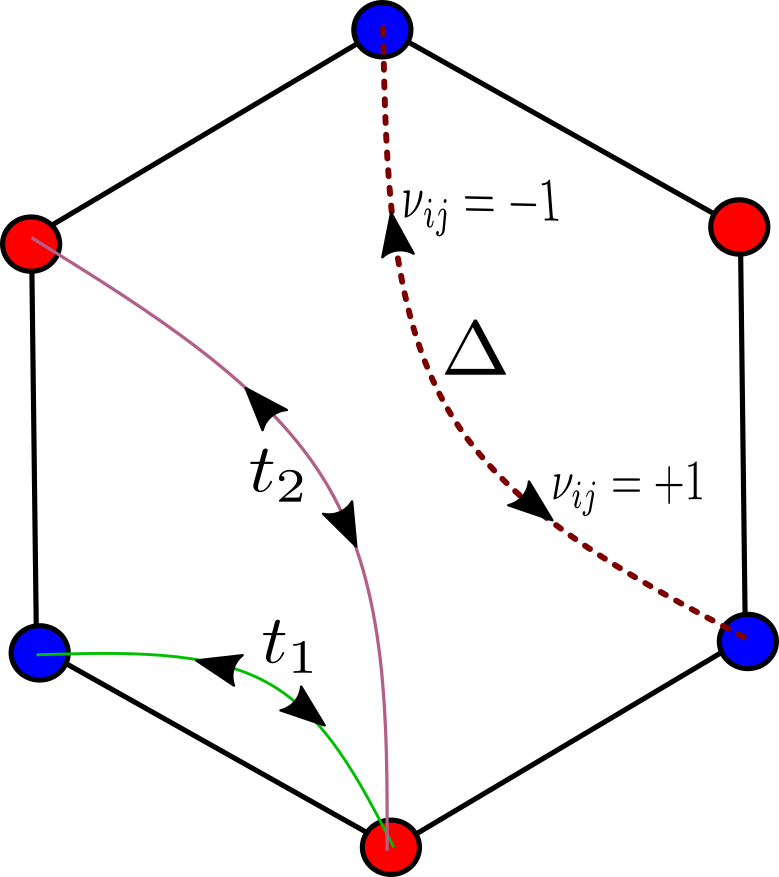
\includegraphics[width=0.5\columnwidth]{../Figures/kmh.png}
\caption{A honycomb cell with NN hopping $t_1$, NNN hopping $t_2$ and intrinsic SOI $\Delta$. $\nu_{ij} = \pm 1$ depending on whether the electron traversing from $i$ to $j$ makes a right ($+1$) or a left turn ($-1$).}
\label{fig:MKMH}
\vspace*{-6pt}
\end{figure}

This corresponds to the case $\bs{\Delta}_{1,ij} = 0$ and $\bs{\Delta}_{2,ij} = (0, 0, i \nu_{ij} \Delta)$ in \ref{BigHam}. The Hamiltonian parameters are sketched in Figure \ref{fig:MKMH}. With this, the effective Hamiltonian will be:

\begin{equation}
\label{MKMHeff}
\hat{H}_{\text{eff}}(t) = \sum_{\langle i,j \rangle} J_{1,ij}\bs{S}_i\bs{S}_j + \sum_{\langle \langle i,j \rangle \rangle} \left\{ J_{2,ij}\bs{S}_i\bs{S}_j + \bs{D}_{2,ij} \bs{S}_i \times \bs{S}_j + \bs{S}_i \bs{\Gamma}_{ij} \bs{S}_j \right\}
\end{equation}

Where:

\begin{align*}
J_{1,ij} &= t_1^2\mathcal{M}(\alpha_{ij}, \text{U}, \omega, t) \\
J_{2,ij} &= t_2^2\mathcal{M}(\alpha_{ij}, \text{U}, \omega, t) \\
\bs{D}_{2,ij} &= - 2\nu_{ij} t_2 \Delta \hat{e}_z \mathcal{M}(\alpha_{ij}, \text{U}, \omega, t) \\
\bs{\Gamma}_{2,ij} &= \Delta^2 \text{diag}(-1,-1,1) \mathcal{M}(\alpha_{ij}, \text{U}, \omega, t) 
\end{align*}

Such a Hamiltonian was first proposed by S. A. Owerre to model honeycome topological magnon insulators \cite{Owerre2016} \cite{Elyasi2018}. Experimental results regarding topological properties of spin waves in honeycomb ferromagnet Cr$I_3$ can only be understood by considering this Hamiltonian \cite{Chen2018}. This model is also relevant for the study of Spin Hall effects of Weyl magnons \cite{Zyuzin2018} \cite{Sekine2016}.

Now, a Hamiltonian with the form $\hat{H} = \sum_{\langle i,j \rangle} J_1 \bs{S}_i\bs{S}_j + \sum_{\langle \langle i,j \rangle \rangle} J_2\bs{S}_i\bs{S}_j$ is known as the $J_1$-$J_2$ Heisenberg model and in a 2D honeycomb lattice it exhibits N\'eel order for $J_2 < J_1 / 6$ and for $J_2 > J_1 / 6$ spin density waves (SDW) appear \cite{Mulder2010}. In the presence of DMI alone there will always be SDW in the plane perpendicular to $\bs{D}$ \cite{Uchida2006}. In Hamiltonian \ref{MKMHeff} we expect SDW to appear in the ground state and the SDW wavevector will be determined by a function of the parameters of this model. In the next section we will do a numerical of study on how modifying the ratio between NN and NNN spin interaction factors can change the spin state of the system.

\end{subsection}

\begin{subsection}{Time independent electric field in the NN + NNN Hamiltonian}

Now, let us examine the case in which the applied electric field is time independent. In this case the effective Hamiltonian is \ref{TimeIndepHeff}, which is the same Hamiltonian obtained when no electric field is applied except for a shift in the intermediate energy by $\pm \omega_0 = e\bs{\vec{R}}_{ij}\bs{\vec{E}}_0$. In this case, if we consider a Hamiltonian such as \ref{BigHam}, we can follow the same procedure done before: we plug in the hopping amplitudes \ref{BigHamHoppingAmp} into \ref{TimeIndepHeff} and apply \ref{SpinRel1} to sum over the spin states and obtain the corresponding spin Hamiltonian. We obtain:

\begin{align}
\hat{H}_{\text{eff}}(t) = &\sum_{\langle i,j \rangle ^*} \left\{ J_{1,ij}\bs{S}_i\bs{S}_j + \bs{D}_{1,ij} \bs{S}_i \times \bs{S}_j + \bs{S}_i\bs{\Gamma}_{1,ij}\bs{S}_j\right\} + \nonumber \\
&\sum_{\langle \langle i,j \rangle \rangle^*} \left\{ J_{2,ij}\bs{S}_i\bs{S}_j + \bs{D}_{2,ij} \bs{S}_i \times \bs{S}_j + \bs{S}_i\bs{\Gamma}_{2,ij}\bs{S}_j\right\}
\end{align}

$\langle i,j \rangle ^*$ denotes sum over NN avoiding repeating the same two sites. The coupling factors are:

\begin{align}
J_{n,ij} &= 4\frac{t_n^2}{U^*_{ij}} \\
\bs{D}_{n,ij} &= 8\frac{t_n i\bs{\Delta}_{n,ij}}{U^*_{ij}} \\
\Gamma_{n,ij}^{\alpha \beta} &= \frac{4}{U^*_{ij}}(\delta_{\alpha \beta} \bs{\Delta}_{n,ij}^2 - 2\Delta_{n,ij}^\alpha\Delta_{n,ij}^\beta )
\end{align}

Where:

\begin{equation}
\frac{1}{U^*_{ij}} =  \frac{1}{2}\left( \frac{1}{\text{U} - e\bs{\vec{R}}_{ij}\bs{\vec{E}}_0} + \frac{1}{\text{U} + e\bs{\vec{R}}_{ij}\bs{\vec{E}}_0} \right)
\end{equation}

\end{subsection}

\end{section}

\begin{section}{Numeric results}
\label{Numerics}

\begin{subsection}{One dimensional system}

We will start with a one dimensional chain with hamiltonian $\hat{H} = \sum_{\langle i,j \rangle} |J_1| \bs{S}_i\bs{S}_j + \sum_{\langle \langle i,j \rangle \rangle} \nu_{ij}|D_2|\hat{e}_z\bs{S}_i \times \bs{S}_j$. This approximated Hamiltonian with no NNN exchange interaction is very simple, but it can describe some systems where it has even been observed $|\bs{D}_{2,ij}| > |J_{2,ij}|$ \cite{Chen2018}. In this case we can write $\bs{S}(r) = S(\cos(kr), \sin(kr), 0)$, where the real number $k$ plays the role of the wavevector, and $\theta = ka-\pi$ is the deviation from the N\'eel state. Then the classical energy per site is given by:

\begin{equation}
\frac{E(\theta)}{2S^2} = -|J_1|\cos(\theta) + |D_2|\sin(2 \theta)
\end{equation}

and the energy is minimized for $\theta^* = \arcsin(\frac{\frac{J1}{D2} - \sqrt{(\frac{J1}{D2})^2+32}}{8})$, i.e. $\theta^* = \theta^*(\frac{J1}{D2})$. Next we will show numerically that the ratio between the NN and NNN parameters, $\frac{J1}{D2}$, can be modulated by the intensity of the field, and therefore the field can be used to control the SDW wavevector. 

We will use the time average approximation \ref{MFactorApprox0} so that we can write:

\begin{align}
J_{1,ij} &= J_{1,ij}^0  \sum_{n} \frac{\mathcal{J}_n(\alpha_{ij})^2}{1+n\frac{\omega}{\text{U}}} \\
D_{2,ij} &= D_{2,ij}^0  \sum_{n} \frac{\mathcal{J}_n(\alpha_{ij})^2}{1+n\frac{\omega}{\text{U}}}
\end{align}

Where $\bs{D}_{2,ij} = \hat{e}_z D_{2,ij}$ and where $J_{1,ij}^0 = J_{1}^0 = \frac{2t_1^2}{\text{U}}$ and $D_{2,ij}^0 = -\frac{4t_2\Delta\nu_{ij}}{\text{U}}$. Since $\mathcal{J}_n(-x) = (-1)^n\mathcal{J}_n(x)$ the dependance is on $|\alpha_{ij}|$ only. Now, using \ref{Def_alpha}, for circularly polarized light we have $|\alpha_{ij}| = \frac{1}{\sqrt{2}}e|\vec{R}_{ij}| \frac{E_0}{\omega} = \frac{1}{\sqrt{2}}ea \frac{E_0}{\omega} \frac{|\vec{R}_{ij}|}{a} = \frac{|\vec{R}_{ij}|}{\sqrt{2}a} \mathcal{E}$, where $a$ is the lattice constant and $\mathcal{E} = \frac{eaE_0}{\omega}$. Now, for $J_{1,ij}$, $i$ and $j$ are NN and so we can write $|\vec{R}_{ij}|=a$, whereas for $D_{2,ij}$, $i$ and $j$ are NNN and so $|\vec{R}_{ij}|=2a$. Thus:

\begin{align}
J_{1,ij} &= J_{1} = J_{1}^0  \sum_{n} \frac{\mathcal{J}_n(\frac{1}{\sqrt{2}}\mathcal{E})^2}{1+n\frac{\omega}{\text{U}}} \\
D_{2,ij} &= D_{2,ij}^0  \sum_{n} \frac{\mathcal{J}_n(\sqrt{2}\mathcal{E})^2}{1+n\frac{\omega}{\text{U}}}
\end{align}

In each case the absolute vale is independent of $i,j$.  Now, in units $\hbar=t_1=1$ we measure energy in units of $t_1$ and frequency in units of $\frac{t_1}{\hbar}$. Then, for $t_2 = 0.1$, $\Delta = 0.5$, $\text{U} = 10$ and $\omega = 6, 16$ we obtain \ref{Fig1:NNvsNNN}. The ratio $\frac{J_{1,ij}}{D_{2,ij}}$ is plotted in \ref{Fig1:ratio}. Finally, in \ref{Fig2} we plot the SDW NN angle $\theta$.

\begin{figure}
\centering
\begin{subfigure}{.45\textwidth}
  %\centering
  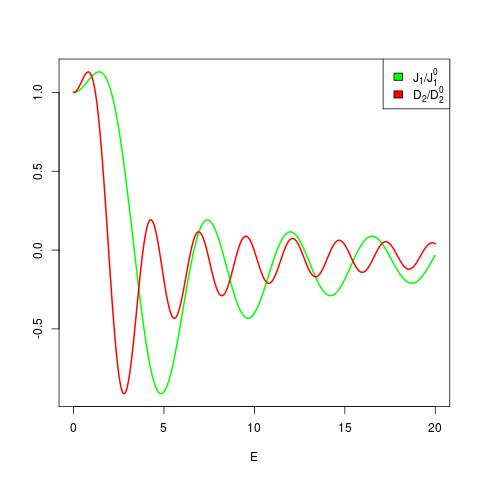
\includegraphics[width=1\linewidth]{Chapters/NNvsNNN.pdf}
  \caption{$\frac{J_{1}}{J_{1}^0}$ and $\frac{D_{2,ij}}{D_{2,ij}^0}$ are plotted as function of $\mathcal{E}$. Similar results are obtained in \cite{Mentink2015} for $J_{1}$. Solid lines are for $\omega = 6$ and dashed lines are for $\omega = 16$.}
  \label{Fig1:NNvsNNN}
\end{subfigure}%
\hspace*{\fill}
\begin{subfigure}{.45\textwidth}
  %\centering
  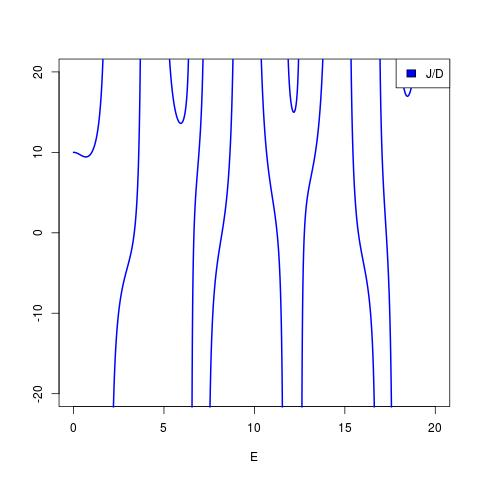
\includegraphics[width=1\linewidth]{Chapters/ratio.pdf}
  \caption{$\frac{J_{1}}{D_{2,ij}}$ is plotted as function of $\mathcal{E}$, it diverges every time $D_{2,ij}$ changes sign. Solid lines are for $\omega = 6$ and dashed lines are for $\omega = 16$.}
  \label{Fig1:ratio}
\end{subfigure}
\label{Fig1}
\end{figure}

\begin{figure}
\centering
  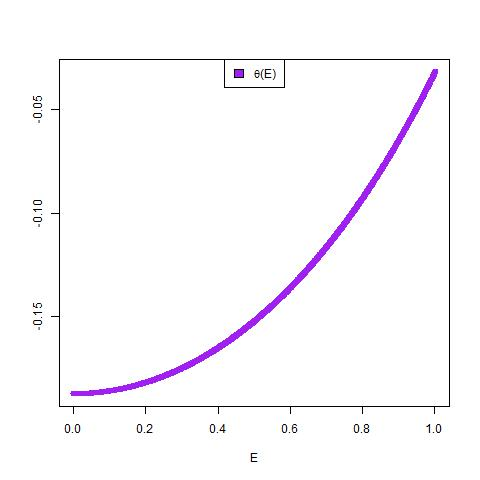
\includegraphics[width=0.5\linewidth]{Chapters/theta.pdf}
  \caption{The spin wave density NN angle $\theta$ as a function of $\mathcal{E}$. The field modifies the ratio $\frac{J_{1}}{D_{2,ij}}$ thus modifying the wave vector. Solid lines are for $\omega = 6$ and dashed lines are for $\omega = 16$.}
\label{Fig2}
\end{figure}

\end{subsection}

\begin{subsection}{Two dimensional systems}
 
In a honeycomb lattice described by \ref{MKMHeff} the usual approach is to write:



\end{subsection}

\end{section}

 
%\chapter{Spin wave theory of antiferromagnets}
\label{SpinWave}

We will start with the Heisenberg antiferromagnet:

\begin{equation}
\hat{H} = J \sum_{\langle i j \rangle} \bs{S}_i \bs{S}_j
\end{equation}

In order to obtain the magnon Hamiltonian for this model we introduce the antiferromagnet Holstein-Primakoff transformation:

\begin{align}
S^+_{Ai} &= \sqrt{2S-\hat{a}^\dagger_i \hat{a}_i} \hat{a}_i \\
S^-_{Ai} &= \hat{a}^\dagger_i\sqrt{2S-\hat{a}^\dagger_i \hat{a}_i}  \\
S^z_{Ai} &= S - \hat{a}^\dagger_i \hat{a}_i \\
S^+_{Bj} &=\hat{b}^\dagger_j\sqrt{2S-\hat{b}^\dagger_j \hat{b}_j} \\
S^-_{Bj} &= \sqrt{2S-\hat{b}^\dagger_j \hat{b}_j} \hat{b}_j \\
S^z_{Bj} &= -S + \hat{b}^\dagger_j \hat{b}_j
\end{align}

Where $A$ and $B$ denote two Ne\'{e}l sublattices and $\hat{a}_i$, $\hat{b}_i$ are bosonic annihilation operators. In the large-S limit we approximate $ \sqrt{2S-\hat{a}^\dagger_i \hat{a}_i} \approx \sqrt{2S}$. Then, the exchange term becomes:

\begin{align*}
\bs{S}_i\bs{S}_j = S_i^zS_j^z + \frac{1}{2}\left(S_i^+S_j^- + S_i^-S_j^+ \right) = S \left( \hat{a}^\dagger_i \hat{a}_i + \hat{b}^\dagger_j \hat{b}_j + \hat{a}_i\hat{b}_j + \hat{a}^\dagger_i\hat{b}^\dagger_j \right) - \hat{a}^\dagger_i \hat{a}_i\hat{b}^\dagger_j \hat{b}_j - S^2
\end{align*}

Now the $S^2$ term is a constant that lowers the energy of the antiferromagnet, therefore is shall not be taken into account to compute the magnon dispersion. The term $\hat{a}^\dagger_i \hat{a}_i\hat{b}^\dagger_j \hat{b}_j$ is zeroth order in $S$ and therefore neglected. We can rewrite the sum over NN as:

\begin{equation}
\sum_{\langle i j \rangle} = 2\sum_{i \in A \delta}
\end{equation}

Where $\delta$ are the NN vectors. Using this, and the Fourier relations:

\begin{align}
\hat{a}_i^\dagger &= \frac{1}{\sqrt{N}} \sum_{\bs{k}} e^{i \bs{k} \cdot \bs{r}_i} \hat{a}_{\bs{k}}^\dagger \\
\hat{b}_j^\dagger &= \frac{1}{\sqrt{N}} \sum_{\bs{k}} e^{i \bs{k} \cdot \bs{r}_j} \hat{b}_{\bs{k}}^\dagger
\end{align}

Where the sum is over $\bs{k}$ in the first Brillouin zone. Using these relations, together with $\sum{i} e^{i{\bs{k}-\bs{k}'}\cdot\bs{r}_i} = \delta_{\bs{k}, \bs{k}'}$ we find:

\begin{equation}
\hat{H} = 2JS \sum_{\bs{k} \bs{\delta}} \left( \hat{a}^\dagger_{\bs{k}}\hat{a}_{\bs{k}} + \hat{b}^\dagger_{\bs{k}}\hat{b}_{\bs{k}} + e^{i\bs{k}\bs{\delta}}\hat{a}_{\bs{k}}\hat{b}_{\bs{-k}} + e^{-i \bs{k}\cdot\bs{\delta}}  \hat{a}^\dagger_{\bs{k}}\hat{b}^\dagger_{-\bs{k}} \right)
\end{equation}

At this point it is common to define $\gamma_{\bs{k}} = \sum_\delta e^{i \bs{k} \cdot \bs{\delta}}$, then denoting $z = \sum_\delta$ we get:

\begin{equation}
\hat{H} = 2JS \sum_{\bs{k}} \left\{ z \left( \hat{a}^\dagger_{\bs{k}}\hat{a}_{\bs{k}} + \hat{b}^\dagger_{\bs{k}}\hat{b}_{\bs{k}} \right) + \gamma_{\bs{k}}\hat{a}_{\bs{k}}\hat{b}_{\bs{-k}} + \gamma_{-\bs{k}}\hat{a}^\dagger_{\bs{k}}\hat{b}^\dagger_{-\bs{k}} \right\}
\end{equation}

Which can be written in matrix form as:

\begin{equation}
\hat{H}_{\bs{k}} = 2JS\begin{pmatrix} 
z & 0 & 0 & \gamma_{\bs{k}} \\
0 & z & 0 & 0 \\
0 & 0 & 0 & 0 \\
\gamma_{-\bs{k}} & 0 & 0 & 0 
\end{pmatrix}
\end{equation}

Acting on the spinor $\Psi_{\bs{k}} = \left(\hat{a}_{\bs{k}},\hat{b}_{\bs{k}},\hat{a}_{-\bs{k}}^\dagger,\hat{b}_{-\bs{k}}^\dagger \right)^T$. That is, $\hat{H} = \sum_{\bs{k}} \Psi_{\bs{k}} \hat{H}_{\bs{k}} \Psi^\dagger_{\bs{k}}$ 

%----------------------------------------------------------------------------------------
%	THESIS CONTENT - APPENDICES
%----------------------------------------------------------------------------------------

\appendix % Cue to tell LaTeX that the following "chapters" are Appendices

% Include the appendices of the thesis as separate files from the Appendices folder
% Uncomment the lines as you write the Appendices

\chapter{Crystal structure and reciprocal lattice}
\label{AP1A}

Here we will introduce some notation. The Bravais lattice in a crystal is the lattice generated by the primitive translations $\bs{a}_\mu$:

\begin{equation}
\bs{R} = \sum_{\mu=1}^3 m_\mu \bs{a}_\mu
\end{equation}
Where $m_\mu$ are integers. The volume of the unit cell is $v = \textbf{a}_1 \cdot (\textbf{a}_2 \times \textbf{a}_3)$. The crystal volume is $V = Nv$ where $N = L_1 L_2 L_3$ is the number of lattice sites. The primitive translations in the reciprocal lattice are defined as $\textbf{b}_1 = \frac{2 \pi}{v}\textbf{a}_2 \times \textbf{a}_3$, etc. With this notation the first Brillouin zone is:

\begin{equation}
\textbf{k} = \sum_{\mu=1}^3 \kappa_\mu \textbf{b}_\mu
\end{equation}
Where $\kappa_\mu = \frac{\nu_\mu}{L_\mu}, -\frac{L_\mu}{2}+1 \leq \nu_\mu \leq \frac{L_\mu}{2}$ so that, $-\frac{1}{2} < \kappa_\mu \leq \frac{1}{2}$. 

In the case of a cubic lattice we have $|\textbf{a}_\mu| = a$ and $|b_\mu| = \frac{2\pi}{a}$ and the vectors of the first Brillouin zone have components $k_\mu = \frac{2 \pi \nu_\mu}{aL}$.

In the next chapters we will also consider the two dimensional honecomb lattice. For this lattice we can choose the primitive translations to be:

\begin{align}
\bs{a}_1 &= \frac{a_0}{2} \left(3, \sqrt{3} \right) \\
\bs{a}_2 &= \frac{a_0}{2} \left(3, -\sqrt{3} \right)
\end{align}
Where $a_0$ is the atom-atom distance (in the case of graphene $a_0 = 1.42 \r{A}$). Each unit cell contains two atoms, dividing the lattice into two sublattices, usually denoted A and B. The reciprocal lattice is defined by the vectors:

\begin{align}
\bs{b}_1 &= \frac{2\pi}{3a_0} \left(1, \sqrt{3} \right) \\
\bs{b}_2 &= \frac{2\pi}{3a_0} \left(1, -\sqrt{3} \right)
\end{align}
These two vectors also span an hexagonal structure. The vectors connecting an atom in the A sublattice to its B sublattice nearest neighbors are:

\begin{align}
\bs{R}^A_1 &= \frac{a_0}{2} \left( 1, \sqrt{3} \right) \\
\bs{R}^A_2 &= \frac{a_0}{2} \left( 1, -\sqrt{3} \right) \\
\bs{R}^A_3 &= a_0 \left( -1, 0 \right)
\end{align}
The vectors connecting an atom in the B sublattice to its A sublattice nearest neighbors are just $\bs{R}^B_i = -\bs{R}^A_i$

\begin{figure}
\centering
  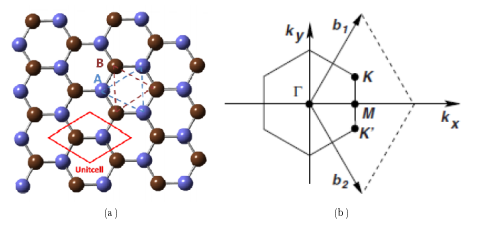
\includegraphics[width=0.7\linewidth]{../Figures/honeycomb_lattice.png}
  \caption{Image from a web source. In Fig. (a) the unit cell is sketched and the sublattices A and B are shown in blue and red respectively. In Fig. (b) the reciprocal lattice is shown, toghether with the high symmetry points $K$, $M$ and $K'$.} 
\label{Fig2.2}
\end{figure}


\chapter{Peierls Substitution}
\label{AP3A}

In first quantization we can introduce a vector potential $\bs{A}(\bs{r},t)$ by changing the Hamiltonian of the lattice \ref{LaticeHam} to:

\begin{equation}
\label{HamEMF}
  \hat{H}'(\bs{r}) = \frac{(\bs{p}-e\bs{A})^2}{2m} +U(\bs{r})
\end{equation}

Now the Bloch functions defined for \ref{LaticeHam} will not be eigenfunctions of this Hamiltonian. We define a new set of Wannier functions in terms of those defined in \ref{Wannier2}, and obtain the new Bloch functions. 

\begin{align}
\psi'_{\bs{R}}(\bs{r}) &= e^{i\frac{e}{\hbar}\int_{\bs{R}}^{\bs{r}} d\bs{r}'\cdot\bs{A}(\bs{r}',t)} \psi_{\bs{R}}(\bs{r}) \\
\phi'_{\bs{k}}(\textbf{r}) &= \frac{1}{\sqrt{M}}\sum_{\bs{R}} e^{-i\bs{k}\cdot\bs{R}}\psi'_{\bs{R}}(\bs{r}) = \frac{1}{\sqrt{M}}\sum_{\bs{R}} e^{-i\bs{k}\cdot\bs{R}} e^{i\frac{e}{\hbar}\int_{\bs{R}}^{\bs{r}} d\bs{r}'\cdot\bs{A}(\bs{r}',t)} \psi_{\bs{R}}(\bs{r})
\end{align}

Where we omitted the band number. The action of the new Hamiltonian is greatly simplified:

\begin{align*}
\hat{H}'(\bs{r}) \psi'_{\bs{R}} (\bs{r}) &= \left[ \frac{(\bs{p}-e\bs{A})^2}{2m} +U(\bs{r}) \right] e^{i\frac{e}{\hbar}\int_{\bs{R}}^{\bs{r}} d\bs{r}'\cdot\bs{A}(\bs{r}',t)} \psi_{\bs{R}}(\bs{r}) = \\
&=e^{i\frac{e}{\hbar}\int_{\bs{R}}^{\bs{r}} d\bs{r}'\cdot\bs{A}(\bs{r}',t)} \left[ \frac{(\bs{p} - i\hbar \bs{\nabla_r}(i\frac{e}{\hbar}\int_{\bs{R}}^{\bs{r}} d\bs{r}'\cdot\bs{A}(\bs{r}',t)) -e\bs{A})^2}{2m} +U(\bs{r}) \right] = \\
&= e^{i\frac{e}{\hbar}\int_{\bs{R}}^{\bs{r}} d\bs{r}'\cdot\bs{A}(\bs{r}',t)} \left[ \frac{\bs{p}^2}{2m} + U(\bs{r}) \right] \psi_{\bs{R}}(\bs{r}) = e^{i\frac{e}{\hbar}\int_{\bs{R}}^{\bs{r}} d\bs{r}'\cdot\bs{A}(\bs{r}',t)} \hat{H}(\bs{r}) \psi_{\bs{R}}(\bs{r})
\end{align*}

And so, the matrix elements as in the case without field except for a phase:

\begin{equation}
\label{PeierlsMtxElem}
t_{ij}(t) = \bra{\psi'_{\bs{R_i}}} \hat{H}'(\bs{r}) \ket{\psi'_{\bs{R_j}}} = e^{i\frac{e}{\hbar}\int_{\bs{R}_j}^{\bs{R}_i} d\bs{r}'\cdot\bs{A}(\bs{r}',t)} \bra{\psi_{\bs{R_i}}} \hat{H}(\bs{r}) \ket{\psi_{\bs{R_j}}}
\end{equation}

When the field can be approximated as constant along the lattice we have: $e^{i\frac{e}{\hbar}\int_{\bs{R}_j}^{\bs{R}_i} d\bs{r}'\cdot\bs{A}(\bs{r}',t)} = e^{i\frac{e}{\hbar} (\bs{R}_i-\bs{R}_j)\cdot \bs{A}(t)}$.

Notice that this substitution also applies if we add a Rashba Spin-Orbit interaction term to \ref{HamEMF}, i.e., if $\hat{H}'(\bs{r}) = \frac{(\bs{p}-e\bs{A})^2}{2m} +U(\bs{r}) + \alpha_R \hat{e}_z\cdot(\hat{\bs{\sigma}} \times (\bs{p}-e\bs{A}))$, then

\begin{align*}
  \alpha_R \hat{e}_z\cdot(\hat{\bs{\sigma}} \times (\bs{p}-e\bs{A})) \psi'_{\bs{R}} &= \alpha_R(\hat{\sigma_x}(\hat{p}_y-e\bs{A}) - \hat{\sigma_y}(\hat{p}_x-e\bs{A})) e^{i\frac{e}{\hbar}\int_{\bs{R}}^{\bs{r}}d\bs{r}'\cdot\bs{A}(\bs{r}',t)} \psi_{\bs{R}} = \\
  &= e^{i\frac{e}{\hbar}\int_{\bs{R}}^{\bs{r}}d\bs{r}'\cdot\bs{A}(\bs{r}',t)} \alpha_R \hat{e}_z\cdot\hat{\bs{\sigma}} \times \bs{p} \psi_{\bs{R}}
\end{align*}

Therefore relation \ref{PeierlsMtxElem} still holds.
\chapter{Identities}
\label{AP3B}
Let $Z(t)$ be an operator dependent on the parameter $t$. Then:

\begin{align*}
d_t e^{Z} &= d_t \sum_{n=0}^\infty \frac{1}{n!} Z^n = \sum_{n=0}^\infty \sum_{m=0}^{n-1} \frac{1}{n!} Z^m \frac{\partial Z}{\partial t} Z^{n-m-1} = \\
&= \sum_{m=0}^\infty \sum_{p=0}^\infty \frac{1}{(m+p+1)!}Z^m \frac{\partial Z}{\partial t} Z^p = \sum_{m=0}^\infty \sum_{p=0}^\infty \frac{m!p!}{(m+p+1)!} \frac{Z^m}{m!} \frac{\partial Z}{\partial t} \frac{Z^p}{p!} =\\
&= \sum_{m=0}^\infty \sum_{p=0}^\infty \int_0^1 dx x^m (1-x)^p \frac{Z^m}{m!} \frac{\partial Z}{\partial t} \frac{Z^p}{p!} = \int_0^1 dx e^{Zx} \frac{\partial Z}{\partial t} e^{Z(1-x)} = \\
&= \int_0^1 dx \sum_{n=0}^\infty \frac{1}{n!} \left[xZ, \dots, \left[xZ, \frac{\partial Z}{\partial t}\right] \dots \right] e^Z = \sum_{n=0}^\infty \frac{1}{(n+1)!} \left[Z, \dots, \left[Z, \frac{\partial Z}{\partial t}\right] \dots \right] e^Z
\end{align*}
Where we used the Beta function $\int_0^1 dx x^m (1-x)^p = \frac{m!p!}{(m+p+1)!}$ and we also used the Baker-Campbell-Hausdorff expansion for $e^{xZ}\frac{\partial Z}{\partial t}e^{-xZ}$ and $\int_0^1 x^n = \frac{1}{n+1}$. Therefore we proved:

\begin{equation}
\label{SneidersID}
d_t e^{Z} = \sum_{n=0}^\infty \frac{1}{(n+1)!} \left[Z, \dots, \left[Z, \frac{\partial Z}{\partial t}\right] \dots \right] e^Z = \sum_{n=0}^\infty \frac{1}{(n+1)!} \text{ad}_Z ^n \left(\frac{\partial Z}{\partial t}\right) e^Z
\end{equation}
Where $\text{ad}_A(B) = [A,B]$.
\chapter{Tight binding model in the honeycomb lattice}
\label{APD}

Graphene, as a representative two dimensional solid with honeycomb lattice structure has some interesting electrical properties induced by its lattice structure. Graphene is a zero gap semiconductor, meaning that its conduction and valence bands touch each other at the $\bs{K}$ points in the momentum space. Around these points the electrons have a linear dispersion relation, resembling that of massless Dirac fermions. In the following we will show this in detail.

Using the same notation introduced in \ref{AP1A} we can introduce the fermionic operators $\hat{a}^\dagger_i$ and $\hat{b}^\dagger_j$ which create and electron on the A and B site receptively, at position $\bs{R}_i$ or $\bs{R}_i$. Then, the tight binding Hamiltonian considering only NN hopping is:

\begin{equation}
\label{TBHex}
\hat{H} = -t\sum_{i \in A}\sum_{\bs{\delta}} (\hat{a}^\dagger_i\hat{b}_{i+\bs{\delta}} + \hat{b}^\dagger_{i+\bs{\delta}}\hat{a}_i)
\end{equation}
Where $i$ labels sites in sublattice A and $\bs{\delta}$ are the NN vectors, we make an abuse of notation by summing $i+\bs{\delta}$ referring, of course, to the site at position $\bs{R}_i+\bs{\delta}$. In order to diagonalize this Hamiltonian we change to momentum space:

\begin{align}
\hat{a}^\dagger_i &= \frac{1}{\sqrt{N}} \sum_{\bs{k}} e^{i\bs{k}\cdot\bs{r}_i}\hat{a}^\dagger_{\bs{k}} \\
\hat{b}^\dagger_j &= \frac{1}{\sqrt{N}} \sum_{\bs{k}} e^{i\bs{k}\cdot\bs{r}_j}\hat{b}^\dagger_{\bs{k}} 
\end{align}
Then \ref{TBHex} reads:

\begin{align*}
\hat{H} &= -\frac{t}{N} \sum_{i \in A}\sum_{\bs{\delta}} \sum_{\bs{k}\bs{k}'} e^{i(\bs{k}-\bs{k}')\cdot\bs{r}_i}e^{-i\bs{k}'\cdot\bs{\delta}} \hat{a}^\dagger_{\bs{k}}\hat{b}_{\bs{k}'} + e^{i(\bs{k}'-\bs{k})\cdot\bs{r}_i}e^{i\bs{k}'\cdot\bs{\delta}} \hat{b}^\dagger_{\bs{k}'}\hat{a}_{\bs{k}} = \\
&= -t \sum_{\bs{\delta}\bs{k}} e^{-i\bs{k}\cdot\bs{\delta}} \hat{a}^\dagger_{\bs{k}}\hat{b}_{\bs{k}} +e^{i\bs{k}\cdot\bs{\delta}} \hat{b}^\dagger_{\bs{k}}\hat{a}_{\bs{k}} = \sum_{\bs{k}} \psi^\dagger(\bs{k})h(\bs{k})\psi(\bs{k})
\end{align*}
Where $\psi(\bs{k}) = \left( \hat{a}_{\bs{k}}, \hat{b}_{\bs{k}} \right)^T$ and:

\begin{equation}
h(\bs{k}) = \begin{pmatrix}
    0 & f(\bs{k}) \\
    f^*(\bs{k}) & 0
\end{pmatrix}
\end{equation}
being $f(\bs{k}) = -t\sum_{\bs{\delta}} e^{i\bs{k}\cdot\bs{\delta}}$. In order to obtain the band structure we need to diagonalize $h(\bs{k})$. This is straightforward and the resulting energy bands are:

\begin{equation}
E_{\pm}(\bs{k}) = \pm|f(\bs{k})| = \pm t\sqrt{3+2\cos(\sqrt{3}k_ya) +4\cos(\sqrt{3}k_y\frac{a}{2})\cos(3k_x\frac{a}{2})}
\end{equation}
The bands will cross, or equivalently the band gap will vanish if $f(\bs{k})=0$ has a solution, which it does at the corners of the first Brillouin zone, i.e. the points:

\begin{align*}
\bs{K} &= \frac{2\pi}{3a}\left( 1, \frac{1}{\sqrt{3}}\right) \\
\bs{K}' &= \frac{2\pi}{3a}\left( 1, -\frac{1}{\sqrt{3}}\right) 
\end{align*}
Where $a$ is the lattice constant. The other corner points are equivalent to either one of these (that is, they can be obtained by a translation of a reciprocal lattice vector).

\begin{figure}
\centering
  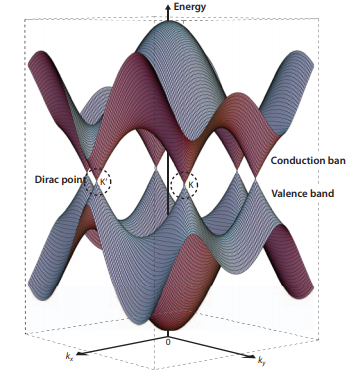
\includegraphics[width=0.7\linewidth]{../Figures/graphene_bands.png}
  \caption{Image from \cite{Ando2009}. The energy bands of graphene.} 
\label{FigD1}
\end{figure}

As depicted in \ref{FigD1} the bands touch in the $\bs{K}$ and $\bs{K}'$ points of the first Brillouin zone. Now, since the system has one electron per atom with two possible spin states it is clear that at zero temperature the lower energy band will be filled (and the upper band will be empty). Thus, the excitations of the system will occur near the crossings at the $\bs{K}$ points. In order to study these excitations it is interesting to linearize the Hamiltonian around these points. Around the $\bs{K}$ point for example, since $f(bs{k})$ vanishes, we can write:

\begin{equation}
h(\bs{K}+\bs{q}) \approx \begin{pmatrix}
    0 & \frac{\partial f(\bs{k})}{\partial \bs{k}}(\bs{K})\cdot\bs{q} \\
    \frac{\partial f^*(\bs{k})}{\partial \bs{k}}(\bs{K})\cdot\bs{q} & 0
\end{pmatrix}
\end{equation}
Now, 

\begin{equation}
\frac{\partial f(\bs{k})}{\partial \bs{k}}(\bs{K})\cdot\bs{q} = -ie^{\frac{2\pi i}{3}} \frac{3a}{2}(q_x+iq_y)
\end{equation}
We can ignore the phase and write:

\begin{equation}
h(\bs{K}+\bs{q}) = v_F \begin{pmatrix}
    0 & q_x+iq_y \\
    q_x-iq_y & 0
\end{pmatrix}
\end{equation}
Where $v_F = \frac{3at}{2}$. This result is usually written in terms of Pauli matrices as:

\begin{equation}
h(\bs{K}+\bs{q}) = v_F(q_x\sigma_x-q_y\sigma_y)
\end{equation}
We can write this more compactly as $h(\bs{K}+\bs{q}) = v_F \left(\bs{q}\cdot\bs{\sigma}\right)^*$. Analogously for the $\bs{K}'$ point we obtain $h(\bs{K}'+\bs{q}) = v_F\bs{q}\cdot\bs{\sigma}$. This result is identical to the massless Dirac Hamiltonian for relativistic electrons where the speed of light is changed to $v_F$. The linearized energy is simply given by $E_{\pm}(\bs{K}+\bs{q}) = \pm v_F|\bs{q}|$. In \cite{Kane2005}, Kane and Mele added a term :
\begin{equation}
h_{SO} = \Delta_{SO}\sigma_z\tau_z s_z
\end{equation} 
to this Hamiltonian (where $\tau_z = \pm 1$ describing states around the $\bs{K}$ or $\bs{K}'$ points respectively and $s_z$ representing the electron's spin). This term leads to an energy $E_{\pm}(\bs{K}+\bs{q}) = \pm \sqrt{\left(v_F\bs{q} \right)^2 + \Delta_{SO}^2}$, i.e. it opens an energy gap $2\Delta_{SO}$. If this gap is large enough, the material becomes insulator in the bulk, while supporting states at the boundaries. This states are known as edge states and are of relevance for the transport of charge and spin.

\chapter{Floquet Theory}
\label{APE}
In this appendix we will state and proof the Floquet theorem and employ the Floquet formalism to derive a perturbative analysis of high frequency time periodic Hamiltonians. This formalism been widely used recently in many-body driven systems (\cite{Desbuquois2017}, \cite{Bordia2017}, \cite{Gorg2018}).

We will start with a periodic Hamiltonian:

\begin{equation}
\hat{H}(t) = \hat{H}(t+T)
\end{equation}

The Floquet theorem states that the eigenstates for the time evolution operator for one period, $\hat{U}(t+T,t)$ can be written as:

\begin{equation}
\label{FloquetMode}
\ket{\psi_n(t)} = e^{-i \epsilon_n t}\ket{u_n(t)}
\end{equation}

Where $\ket{u_n(t+T)} = \ket{u_n(t)}$ is a periodic function, called Floquet mode, and $\epsilon_n$ is a real number known as the quasienergy. To show this, let $a_n(t)$ be the eigenvalue of $\ket{\psi_n(t)}$ under $\hat{U}(t+T,t)$, that is $\hat{U}(t+T,t)\ket{\psi_n(t)} = a_n(t)\ket{\psi_n(t)}$, then by multiplying this equation by $\hat{U}(t',t)$ from the left and using the periodicity of the Hamiltonian in $\hat{U}(t',t) = \hat{U}(t'+T,t+T)$ we obtain:

\begin{align*}
\hat{U}(t'+T,t) \ket{\psi_n(t)} &= a_n(t)\ket{\psi_n(t')} \rightarrow \\
\hat{U}(t'+T,t) \hat{U}(t,t')\hat{U}(t',t) \ket{\psi_n(t)} &= a_n(t)\ket{\psi_n(t')} \rightarrow \\
\hat{U}(t'+T,t') \ket{\psi_n(t')} &= a_n(t)\ket{\psi_n(t')}
\end{align*}

Which means that $a_n(t') = a_n(t)$, so the eigenvalue does not depend on time, and since it is an eigenvalue of an unitary operator it can be written as $a_n = a_n(t) = e^{-i\epsilon_nT}$ for certain real number $\epsilon_n$. Therefore, we have 

\begin{align*}
\ket{\psi_n(t+T)} &= e^{-i\epsilon_nT} \ket{\psi_n(t)} \rightarrow \\
\ket{\psi_n(t)} &= e^{-i\epsilon_nt} \ket{u_n(t)}
\end{align*}

For $\ket{u_n(t)} = e^{i\epsilon_nt} \ket{\psi_n(t)} = \ket{u_n(t+T)}$, and this proves the theorem. The states $\ket{\psi_n(t)}$ are called Floquet states and are solutions of the time dependent Schr\"{o}dinger equation $i\text{d}_t\ket{\psi_n(t)} = \hat{H}(t)\ket{\psi_n(t)}$. The time evolution operator can be written as:

\begin{equation}
\hat{U}(t_2,t_1) = \sum_n e^{-i\epsilon_n(t_2-t_1)}\ket{u_n(t_2)}\bra{u_n(t_1)}
\end{equation}

Therefore the time evolution of a superposition of Floquet states will be determined by two different contributions:

\begin{itemize}
\item The periodic evolution of the superposing Floquet modes. This is called micromotion.
\item The non-periodic dephasing due to the factor $e^{-i\epsilon_n(t_2-t_1)}$ depending on the quasienergies $\epsilon_n$.
\end{itemize} 

It is interesting to study these two time dependencies separately. With his purpose we define the micromotion operator and the Floquet Hamiltnian. The micromotion operator is defined as:
\begin{equation}
\hat{U}_F(t_2,t_1) \equiv \sum_n \ket{u_n(t_2)}\bra{u_n(t_1)}
\end{equation}
so that $\ket{u_n(t_2)} = \hat{U}_F(t_2,t_1)\ket{u_n(t_1)}$, i.e. it is responsible of the periodic time evolution intrinsic of the Floquet modes. On the other hand, the Floquet Hamiltonian $\hat{H}_{t_0}^F$ is a time-independent Hamiltonian defined such that:
\begin{equation}
e^{-iT\hat{H}_{t_0}^F} \equiv \hat{U}(t_0+T,t_0)
\end{equation}
or equivalently:
\begin{equation}
e^{-it\hat{H}_{t_0}^F} = \sum_n e^{-i\epsilon_nt}\ket{u_n(t_0)}\bra{u_n(t_0)}
\end{equation}
this Hamiltonian will time-evolve states by adding a phase $e^{-i\epsilon_n(t_2-t_1)}$ to the correspondent fixed-time modes. The full time evolution operator is a combination of both time evolutions:
\begin{align*}
\hat{U}(t_2,t_1) &= \sum_n e^{-i\epsilon_n(t_2-t_1)}\ket{u_n(t_2)}\bra{u_n(t_1)} = \\
&\left( \sum_n e^{-i\epsilon_n(t_2-t_1)}\ket{u_n(t_2)}\bra{u_n(t_2)} \right)\left( \sum_n\ket{u_n(t_2)}\bra{u_n(t_1)}\right) = \\
&\left( \sum_n \ket{u_n(t_2)}\bra{u_n(t_1)} \right)\left( \sum_n e^{-i\epsilon_n(t_2-t_1)}\ket{u_n(t_1)}\bra{u_n(t_1)} \right)
\end{align*}
That is:
\begin{equation}
\hat{U}(t_2,t_1) = e^{-i(t_2-t_1)\hat{H}_{t_2}^F}\hat{U}_F(t_2,t_1) = \hat{U}_F(t_2,t_1)e^{-i(t_2-t_1)\hat{H}_{t_1}^F}
\end{equation}

\section{Extended Hilbert space}

Having introduced the micromotion operator and the Floquet Hamiltonian, we turn on to introduce the concept of extended Hilbert space. Introducing \ref{FloquetMode} in the Scr\"{o}dinger equation we get:

\begin{equation}
\left[ \hat{H}-i\text{d}_t\right] \ket{u_n(t)} = \epsilon_n\ket{u_n(t)}
\end{equation}

This can be regarded as an eigenvalue problem in the space $\mathcal{F}=\mathcal{H}\otimes\mathcal{L}_T$, where $\mathcal{L}_T$ is the space of square integrable T-periodic functions. The operator $\hat{Q} = \hat{H}-i\text{d}_t$ acting on $\mathcal{F}$ is referred to as the quasienergy operator. States in the extended Hilbert space (that is, a state plus its periodic time dependence) is usually denoted as $\ket{u}\rangle$, and the inner product in this space is defined as:

\begin{equation}
\langle \bra{u}\ket{v} \rangle = \frac{1}{T}\int_0^T \text{d}t \bra{u(t)}\ket{v(t)}
\end{equation}

An orthonormal basis for the extended Hilbert space can be obtained as the direct product an orthonormal basis of $\mathcal{H}$ and $\mathcal{L}_T$. A convenient orthonormal basis for $\mathcal{L}_T$ is given by the functions $e^{im\omega t}$, therefore, if $\ket{\alpha}$ labels an orthonormal basis of $\mathcal{H}$, then the set of functions $\ket{\alpha m (t)} = \ket{\alpha}e^{im\omega t}$ is a basis of the extended Floquet space, and it is denoted as $\ket{\alpha m}\rangle$. In this basis, the quasienergy operator has matrix elements:

\begin{align}
\langle \bra{\alpha' m'}\hat{Q}\ket{\alpha m} \rangle &= \frac{1}{T}\int_0^T \text{d}t e^{-im'\omega t}\bra{\alpha'} \hat{H}(t)-i\hbar\text{d}_t \ket{\alpha}e^{im\omega t} = \nonumber \\
&= \bra{\alpha'} \hat{H}_{m'-m} \ket{\alpha} + \delta_{m'm}\delta_{\alpha' \alpha}m\hbar\omega \label{QOmatelem}
\end{align}

Where
\begin{equation}
\hat{H}_m = \frac{1}{T}\int_0^T \text{d}t e^{-im\omega t}\hat{H}(t) 
\end{equation}
is the Fourier transform of the Hamiltonian. Now, a Floquet state $\ket{\psi_n(t)} = e^{-i \epsilon_n t}\ket{u_n(t)}$ can be expanded as $\ket{u_n(t)} = \sum_m e^{im\omega t}\ket{u_{nm}}$, using \ref{QOmatelem} and projecting onto the \textit{m}th Fourier mode we can rewrite the Scr\"{o}dinger equation as:

\begin{equation}
(\epsilon_n+m\omega)\ket{u_{nm}} = \sum_{m'}\hat{H}_{m-m'}\ket{u_{nm'}}
\end{equation}




















%----------------------------------------------------------------------------------------
%	BIBLIOGRAPHY
%----------------------------------------------------------------------------------------

\printbibliography
%[heading=bibintoc]

%----------------------------------------------------------------------------------------

\end{document}  
